\documentclass[
		a4paper,
		12pt,
		twoside,
		openany,        % Chapter beginnen auf rechter Seite
		parskip,
    % tocbasic,
		final,          % DEBUG modus
		11pt,
    % draft, # DEBUG MOUS
		appendixprefix,
    % headsepline,                       % Linie nach Kopfzeile.
    % footsepline,                       % Linie vor Fusszeile.
    % bibtotocnumbered,                  % Literaturverzeichnis im Inhaltsverzeichnis nummeriert einfügen.
		chapterprefix,  % Kapitel anschreiben als Kapitel
]{scrreprt}
\usepackage[twoside,width=14cm, height=24cm,right=3.25cm, left=2.5cm]{geometry}
\setlength{\marginparwidth}{2.25cm}
\clubpenalty = 10000
\widowpenalty = 10000 \displaywidowpenalty = 10000

\usepackage[ngerman]{babel}

\usepackage[utf8]{inputenc}		%Damit kann man auch Umlaute direkt eintippen  \o/
\usepackage{textcomp}
\usepackage{amsmath}
\usepackage{amssymb}
\usepackage{amsbsy}
\usepackage{amsfonts}
\usepackage{amsthm}
\usepackage{graphicx}	%including images
\usepackage{fancyhdr}	%for editiable headers and footers
\usepackage{setspace} 	%for 1,5times row space
\usepackage{color}
\definecolor{darkblue}{rgb}{0,0,.5}
\usepackage[colorlinks,
  pdfpagelabels,pdfstartview=FitH,bookmarksopen=true,bookmarksnumbered=true,
  linkcolor= black,
  plainpages=false,
  hypertexnames=false,
  citecolor=black,linkcolor=black,menucolor=black,urlcolor=darkblue]
  {hyperref}
			%clickable TOC
\usepackage{multirow}	%linebreak in Table
\usepackage{enumerate}	% \begin{enumerate}[a.]     Custom Nummerierung
\usepackage{float}	% Images mit Float
\usepackage{colortbl}	%colorTables
\usepackage{framed}   		%begin{framed}
\usepackage{longtable} 		%begin{longtable}
\usepackage{makeidx}
\usepackage[square,sort&compress,comma,numbers]{natbib}  % natbib, aber Zitiert mit [..] anstatt (..)
\usepackage{epigraph}		% Epigraph = stylische Zitatte
\usepackage{listings}	% Quellcode Listings und List of Listings
\usepackage{caption}	% Modifizierung und setzen von custom captions
\usepackage[dvipsnames,table]{xcolor}
\usepackage[nottoc]{tocbibind}	% TOC Plugin -> ??
\usepackage{relsize}
\usepackage[toc]{glossaries}
%\usepackage{marginnote}
%\usepackage{minted}  % TODO Pygments wrapper... ohje :)



%%%%%%%%%%%%%%%%%%%%%%%%%%%%%%%5
%% Metainfos
%%%%%%%%%%%%%%%%%%%%%%%%%%%%%%%

\newcommand{\ownTitle}{Diplomarbeit}
\newcommand{\ownTitleZ}{Testgetriebene Entwicklung von Web-Serveranwendungen auf der Basis von Ruby on Rails}
\newcommand{\ownAutor}{Stefan Wienert, HTW Dresden}

\title{\ownTitle}
\author{\ownAutor}
\pdfinfo{
 /Title  (\ownTitle)
 /Author (\ownAutor)
 /Subject (\ownTitleZ)
 /Keywords()
}
\date{\today}
\setlength{\epigraphwidth}{.8\textwidth}


%%%%%%%%%%%%%%%%%%%%%%%%%%%%%%%%%%
%% HEAD AND FOOTLINES
%%%%%%%%%%%%%%%%%%%%%%%%%%%%%%%%%%
\pagestyle{headings}
\definecolor{Gray}{rgb}{0.85,0.85,0.90}

\makeindex 	%start Aufzeichnung eines Stichwortverzeichnisses
\makeglossary  	%start Aufzeichnung eines Glossars

%%%%%%%%%%%%%%%%%%%%%% STYLINGS & FONTS %%%%%%%%%%%%%%%%%%%%%%%%%%%%
\renewcommand{\footrulewidth}{0.5pt}
%\let\cleardoublepage\clearpage
\parskip 5pt       % sets spacing between paragraphs
\parindent 0pt


\usepackage{bookman}  % 118 pages, sehr sauber
% \usepackage{newcent}  % 116 pages, nice aber etwas zu kraeftig
% \usepackage{lmodern}  % 109 pages, standardmaessig
% \usepackage{boisik}    % 113 pages, gewagt aber sehr detailiert, etwas ungerade
% \usepackage{palatino}    % 111 pages, Arial'y sehr langweilig in den Ueberschriften
% \usepackage{cmbright}    % 111 pages, Wie ein modernes Buch. Gut fuer ne Doku oder so
 \usepackage{charter}    % 109 pages, Wie ein modernes Buch. Gut fuer ne Doku oder so
%\fontsize{12}{15}

\usepackage{hyphenat}
\usepackage[T1]{fontenc}


\hyphenation{
Com-mu-ni-ty
Soft-ware-Ent-wick-lung
Soft-ware
Aus-für-lich
Um-for-mu-lie-rung
Test-fall-ab-deck-ung
Test-Unit
Test/Unit
Da-ten-bank-an-bin-dung
Tes-ten
Grob-ent-wurf
Pro-gram-ming
Active-Record
Ini-ti-ali-sie-rung
Sys-tem
be-schreibt
De-ckungs-gleich-heit
}

\usepackage{setspace}
\setstretch{1,15} % Mein TOC ist zu lang!!
\newcommand{\fullref}[1]{\ref{#1} -- \glqq\,\textit{\nameref{#1}}\grqq}
% Shadowbox

\xdefinecolor{B4}{cmyk}{.25,.05.5,0,0}
%\xdefinecolor{B4}{rgb}{0.9,0.9,1}
\xdefinecolor{S10}{cmyk}{0 ,0, 0,.1}

\usepackage{tikz}
\usetikzlibrary{shadows}
\newcommand{\shadebox}[1]{%
\vspace{1\baselineskip}%
\noindent%
\begin{tikzpicture}%
\node at (0,0) [
   anchor=north west, 
    rounded corners,
   minimum width={\linewidth-1ex},
   draw=B4,
   fill=B4,
   copy shadow={
             shadow xshift=1ex,
             shadow yshift=-1ex,fill=S10,draw=white}
  ] 
{\parbox{0.9\linewidth}{#1}};
\end{tikzpicture}\vspace{1\baselineskip}}




\newcommand{\cbox}{\includegraphics[width=0.2cm]{material/cbox.png} \ }
\newcommand{\imgsource}[1]{\captionsetup{font={footnotesize,bf,it}}
 \caption*{#1}}

% \setcounter{tocdepth}{2}	%kleineres TOC
\newcommand{\arr}{$ \Longrightarrow$}


% Listings fuer Ruby

\lstloadlanguages{Ruby}
\lstset{%
  basicstyle=\ttfamily\footnotesize\color{black},
  commentstyle = \ttfamily\color{gray},
  keywordstyle=\ttfamily\color{blue},
  stringstyle=\color{red},
  showspaces=false,               % show spaces adding particular underscores
  showstringspaces=false, 
  frame=single,
  breaklines=true
}
\lstset{literate=%
{Ö}{{\"O}}1
{Ä}{{\"A}}1
{Ü}{{\"U}}1
{ß}{{\ss}}2
{ü}{{\"u}}1
{ä}{{\"a}}1
{ö}{{\"o}}1
}

\newglossaryentry{test} {
  name={Test},
  description= {\index{Test}oder Testfall ist eine, meist automatisierte, Prüfung des Programmverhaltens bei definierten Eingabeparametern},
  plural=Tests
}

\newglossaryentry{testrunner} {
  name={Test-Runner},
  description= {oder Testtreiber) ist eine Software, um \glossarpl{test} aufzurufen und deren Ausführung zu überwachen und zu steuern}
}

\newglossaryentry{testsuite} {
  name={Test-Suite},
  description= {ist eine Gruppe von mehreren Testfällen für eine Komponente oder das für gesamte System}
}

\newglossaryentry{fehler} {
  name={Software-Fehler},
  description= {oder Defekt, ist ein unerwartetes Verhalten der Software, der zu einem Versagen der Software führen kann},
text=Fehler,
first={Software-Fehler}
}
\newglossaryentry{quality} {
  name={Code-Qualität},
  description= {beinhaltet die Software-Qualitäten Lesbarkeit, Testbarkeit, Wartbarkeit, Erweiterbarkeit, geringe Komplexität},
}

\newglossaryentry{metrik} {
  name={Code-Metrik},
  plural={Code-Metriken},
  description={Eine Softwaremetrik ist das Ergebnis einer statischen oder dynamischen Codeanalyse zur Generierung von Informationen über den Quelltext. Beispiele: Testabdeckung, Anzahl Codezeilen, Anzahl \glossarpl{smell} pro Codezeile}
}
\newglossaryentry{refaktorisieren} {
  name = {Refaktorisieren},
  description = {Ist eine Modifikation des Programmcodes ohne Modifikation des externen Verhaltens um nicht-funktionale Eigenschaften des Quellcodes zu verbessern, wie z.B. Lesbarkeit, Wiederverwendbarkeit, Wartbarkeit}
}
\newglossaryentry{Testabdeckung} {
  name=Testabdeckung,
  description={auch: \index{Test!Testabdeckung}Testausführungsabdeckung, Überdeckungsgrad, Testfallabdeckung. Eine dynamische Code-Metrik\index{Code-Metrik}, die angibt, welche Codezeilen durch keinen Test abgedeckt wurde. Es wird unterschieden in die Stufen C0, C1 und C2 mit steigender Komplexität der Messung. Details im Abschnitt \ref{sec:metrics}},
  first = {Testabdeckung}
}
\newglossaryentry{TDD}{
  name={Testgetriebene Entwicklung},
  description={englisch Test Driven Development/Test Driven Design, Ausführlich dargelegt in Abschnitt \ref{sec:tdd}},
  text = TDD,
  first = {Testgetriebene Entwicklung}
}
\newglossaryentry{BDD}{
  name={ Behavior Driven Development},
  description={ (Verhaltensgetriebene Entwicklung). Umformulierung von TDD\index{TDD} zur Ausrichtung auf Businessprozesse. Das Vokabular zielt auf die Spezifikation von Erwartungen im Systemverhalten, anstatt Definition nachträglicher Tests}
}
\newglossaryentry{CRUD} {
  name={CRUD},
  description={Create, Read, Update, Delete sind die vier Basisoperationen, die auf persistente Speicherung ausgeführt werden können.},
  first={Create Read Update Delete (CRUD)}
}
\newglossaryentry{smell}{
  name={Code Smell},
  description={oder Bad Smell\index{Code-Smell}. Ist ein Anzeichen für eine suboptimale Quelltextstelle, die auch ein Hinweis auf ein größeres Designproblem sein kann. Oft auch ein Kandidat für ein Refaktoring. Informationen zu Smells und deren Refaktorisierung\index{Refaktorisierung} sind im Buch von M.Fowler zu finden \citep{fowler_refactoring_1999}},
  plural={Code Smells}
}
\newglossaryentry{ORM}{
  name={ORM},
  description={Objektrelationales Mapping, ist eine Persistenztechnik, um Objekte transparent in einer Datenbank zu speichern und umgekehrt, Tabellenzeilen in Objekte wieder rückzuübersetzen},
  plural={ORMs},
  first={Objekt-relationales Mapping (ORM)}
}
\newglossaryentry{MVC}{
  name={MVC},
  description={Model-View-Control, ist ein \glossar{patterns}, das insbesondere bei GUI- und Web-Anwendungen beliebt ist. Rails\index{Ruby-on-Rails} basiert auf dem MVC-Muster},
  plural={MVCs},
  first={Model-View-Controller (MVC)}
}

\newglossaryentry{rails}{
  name={Ruby on Rails},
  description={ist ein auf der Programmiersprache Ruby basierendes Web-Framework und ist Gegenstand des Kapitel \ref{sec:rails}}
  text = Rails,
  first = Ruby on Rails
}

\newglossaryentry{Test-Double} {
  name={Test-Double},
  plural={Test-Doubles},
  description = {haben die Aufgabe, komplexe Objekte in einem isolierten Test \index{Test}zu simulieren, in dem statt komplexer Berechnungen oder externer Zugriffe konstante Werte geliefert werden. Vertreter dieser Test Doubles sind die Mock\index{Test-Double!Mock}s und Stub\index{Test-Double!Stub}s, siehe Abschnitt
 \ref{sec:mocks}}
}
\newglossaryentry{patterns}{
  name={Entwurfsmuster},
  description={ oder Design Patterns sind bewährte Vorlagen, um häufig wiederkehrende Probleme zu lösen. Weitere Informationen im Buch Design Patterns: Elements of Reusable Object-Oriented Software von Gamme, Helm, Johnson, Vlissides (Gang of Four)}
}
\newglossaryentry{RSS}{
  name={RSS},
  description={  RDF Site Summary, ist ein standardisierter XML-Dialekt zur maschinenlesbaren Verteilung und Veröffentlichung von Inhalten. Es existiert in den Versionen 0.9 bis 2.0.1, die sich nur in Details, wie z.B. Einbindung von Rich-Media (Podcasts, ..) und Namespaces unterscheiden}
}
\newglossaryentry{Test-Umgebung} {
  name={Test-Umgebung},
  description={ist eine spezielle Konfiguration der Hard- und Software, um Tests unter kontrollierten und bekannten Bedingungen auszuführen. Dies beinhaltet neben dem zu testenden Objekten (Object under Tes) auch sogenannte \glossarpl{Test-Double}\index{Test-Double} und den \glossar{testrunner}}
}
\newglossaryentry{gem} {
  name={Gem},
  plural={Gems},
  description={als Gem\index{Gem}s (zu deutsch: Edelsteine) werden in der Ruby-Gemeinschaft Bibliotheken Dritter bezeichnet, die in einem zentralem Repository lagern. Das Bekannteste dieser Repositorys ist rubygems.org. Nahezu alle Ruby-Bibliotheken lassen sich hier finden und innerhalb von Sekunden mittels des Kommandozeilenwerkzeuges gem installieren. Beispielsweise ließe sich \glossar{rails} mittels \texttt{gem install rails} installieren}
}

\newglossaryentry{DSL} {
  name={DSL},
  plural={DSLs},
  description={Eine Domain-spezifische Sprache ist eine auf eine spezielle Problemdomäne ausgerichtete Programmier- oder Spezifikationssprache. Vertreter sind z.B. SQL, die Statistiksprache R oder die Hardwarebeschreibungssprache VHDL. Sie stehen damit den Allzweck-Programmiersprachen gegenüber},
  first={Domain-Specific-Language (DSL)}
}


\newglossaryentry{CMS} {
  name={CMS},
  plural={CMSe},
  description={Content Management System (Inhaltsverwaltungssystem) ist eine, meist webbasierte Software, die es Nutzern ermöglicht einfach statische Inhalte anzulegen und zu bearbeiten},
first = {Content Management System}
}
\newcommand{\glossar}[1]{$^\uparrow$\gls{#1}}

\newcommand{\glossarpl}[1]{$^\uparrow$\glspl{#1}}
\glsaddall

\renewcommand{\glossarypreamble}{Im Folgenden werden einige oft verwendete Begriffe näher erläutert. Innerhalb des Hauptteils dieser Arbeit sind diese Begriffe mit einem $^\uparrow$ gekennzeichnet.}
% \renewcommand{\glossarymark}{Glossar}

\printglossary[toctitle=Glossar]

  % Glossar definitions

\begin{document}
 \include{parts/partials/frontpage}
 \cleardoublepage

 \pagenumbering{Roman}
 \tableofcontents		%Inhaltsverzeichnis
 \newpage
 \setstretch{1,25}  % Entspricht \onehalfspacing
 \chapter*{Danksagung}

Besonderen Dank gilt meinem Betreuer, Prof. Fritzsche, der sich regelmäßig und ausführlich mit meiner Arbeit beschäftigte und mir wertvolle Hinweise erteilte.

Mein Dank gilt auch der Fakultät Informatik und Prof. Wiedemann für das zur Verfügung gestellte Büro, der Bibliothek der HTW-Dresden und Prof. Nestler für das Bestellen von tagesaktueller Literatur.

Ich danke auch meiner Frau, die mich während des Schreibens unterstützt hat und bei der Erstellung der Grafiken Tipps gab. Für die orthografische und expressive Optimierung sei meinen Freunden Daniel Schäufele, Jörg Sachse, Martin Schneider, Akos Toth und Stefan Koch gedankt.

Diese Arbeit entstand in Zusammenarbeit mit der Firma pludoni GmbH und unter Aufsicht des Geschäftsführers Dr. Jörg Klukas. Ich danke ihm für die Möglichkeit, frei zu arbeiten und viele neue Dinge auszuprobieren und für das Vertrauen, das er dabei in mich gesetzt hat.



  % Table -- Zebrastreifen und 1.25 Row Abstand
  \rowcolors{1}{lightgray!50!white}{white}
  \colorlet{tableheadcolor}{gray!40}
  \renewcommand\arraystretch{1.25}% (MyValue=1.0 is for standard spacing)


  \thispagestyle{empty} \mbox{}
  %\newpage
  %\setcounter{page}{-1}
  %\clearpage
  \cleardoublepage
  \pagenumbering{arabic}
 \newpage\chapter{Einleitung}

Das \randbem{Testgetriebene Entwicklung...}Hauptthema dieser Diplomarbeit, die Testgetriebene Entwicklung, ist vielen Programmierern vom Namen her bekannt. Ungeachtet dessen, dass  viele Studien über die (positiven) Auswirkungen über diesen Entwicklungsansatz  existieren, so wird sie trotzdem relativ selten eingesetzt und es existieren große Vorbehalte, wie z.B. dass es Zeitverschwendung sei oder dass Programmierer fälschlicherweise annehmen, sie könnten die Komplexität überschauen\footnote{\url{http://tamasgyorfi.wordpress.com/tag/excuses-to-tdd/}}.\\
Diese, teilweise mythenumrankte, Technik hat innerhalb des Entwicklerteams der pludoni GmbH ein großes Interesse geweckt und wird aus diesem Grund nun näher untersucht.

Die \randbem{...von Webserveranwendungen...}pludoni GmbH benötigt für ihre Services gut funktionierende und effizient entwickelte Webserveranwendungen. Das Framework Ruby on Rails\index{Ruby-on-Rails} scheint dafür wie geschaffen und erste kleinere Erfahrungen waren durchaus positiv. Durch eine vielbestätigte effektive Entwicklung, ist Rails ideal für den Einsatz in kleinen Teams, wie das Entwicklerteam der pludoni GmbH eines ist, geeignet.

Dieses Framework \randbem{...auf Basis von Ruby on Rails} ist das zweite große Thema dieser Diplomarbeit. Rails und Testen passen anscheinend sehr gut zusammen, da das Testen im Allgemeinen in der Ruby-Community einen sehr hohen Stellenwert hat. Außerdem existiert eine Vielzahl von Testwerkzeugen und die meisten bekannten Bibliotheken verfügen über ausgiebige Tests. Damit passen die Testgetriebene\index{TDD} Entwicklung und Ruby (on Rails) perfekt zusammen.

Um die Auswirkungen der Testgetriebene\index{TDD}n Entwicklung besser nachzuvollziehen können, benötigt man ein Messinstrument. Dafür sind in diesem Kontext der Webentwicklung die Code-Metrik\index{Code-Metrik}en geeignet. Sie können einen groben Überblick über den Zustand des Quellcodes geben. Daher sind sie ideal, insbesondere in der Lernphase der Testgetriebenen Entwicklung, Feedback zu geben.

Wie das Zusammenspiel von Ruby (on Rails\index{Ruby-on-Rails}), der Testgetriebene\index{TDD}n Entwicklung und der Einsatz von Code-Metrik\index{Code-Metrik}en praktisch erfolgen, wird in dieser Arbeit im Detail betrachtet und mit eigenen praktischen Erfahrungen belegt.

\section{Motivation}

Kurz nach der Firmengründung der pludoni GmbH absolvierte der Autor dort sein Pflichtpraktikum und war danach weiterhin als Werkstudent tätig.
Während dieser Zeit nahmen Programmierer verschiedener Erfahrungsstufen und auch Praktikanten an der Neu- und Weiterentwicklung der Webserversoftware teil. Dies hat zur Folge, dass die Komplexität der Software inzwischen ein Level erreicht hat, bei dem das Maß an Regressionsfehlern\footnote{fehlerauslösender Quelltextänderungen} stark anstieg.

Da zum großen Teil keine automatisierten Softwaretests geschrieben wurden, lassen sich diese nur schwer auffinden. Ein Versuch, nachträglich Softwaretests hinzuzufügen, wurde evaluiert und als zu aufwändig befunden, da der Code in seinem jetzigen Zustand nur äußerst schwer zu testen ist. Gründe dafür sind suboptimale Codestrukturen (Spaghetticode), die schwer bis unmöglich zu testen sind. Hier müsste zuerst refaktorisiert werden, aber da keine Tests vorhanden sind, ist dies aufgrund der Regressionsfehler riskant. %Ein Teufelskreis!

Für ein neues Projekt, it-jobs-und-stellen.de, soll dies nun mit einem anderen Ansatz verlaufen.

Neben der Umstellung auf ein modernes Web-Framework, sollen nun Tests im Einklang zum Code erstellt werden, um auf Knopfdruck  umfassende Informationen über den Systemzustand zu erhalten, wie sie ein manueller Test \index{Test}in der Gründlichkeit und Schnelligkeit niemals erreichen kann. Außerdem besteht die Hoffnung auf eine nachhaltige Verbesserung der Code-Qualität, um in Zukunft flexibel auf Änderungen reagieren zu können.


\subsection{Die pludoni GmbH}

Die pludoni GmbH ist ein junges dynamisches Dresdner Unternehmen, welches sich zum Ziel gesetzt hat, lokale Communitys zur gegenseitigen Fachkräfteempfehlung aufzubauen und zu betreuen sowie Tools für die Vereinfachung der Personalarbeit mittelständischer Unternehmen zu entwickeln. Einige Beispiele für diese Communitys sind zur Zeit ITsax.de, ITmitte.de und MINTsax.de\footnote{http://www.itsax.de/, http://www.itmitte.de, http://www.mintsax.de/}.
\marginline{\includegraphics[width=0.8\marginparwidth]{material/pludoni.png}\\\centering pludoni GmbH}
\paragraph{Funktionsweise der Communitys}
Die Communitys bestehen jeweils aus einer Anzahl mittelständischer Unternehmen einer Branche, Bildungseinrichtungen sowie Vertetern von Städten und Vereinen. Für ITsax.de ist das die IT-Branche. Neben diesem Branchenfokus sammeln sich nur Unternehmen einer spezifischen Region. Bei ITsax.de sind dies Mittel- und Ostsachsen, bei ITmitte.de z.B. Mitteldeutschland, d.h. Thüringen, Sachsen-Anhalt und Westsachsen.
\begin{table}[htbp]
\label{tb:dt}
\caption{Übersicht über pludoni Communitys. Stand September 2011}
\begin{tabular}{|l|p{3.8cm}|p{5cm}|l|}
\hline
\rowcolor{Gray}
Community & Branche & Region & Mitglieder \\\hline
ITsax.de & IT, Software &  Sachsen (Fokus Süden und Osten) & 63\\\hline
ITmitte.de & IT, Software &  Mitteldeutschland (Thüringen, Sachsen-Anhalt, Westsachsen) & 57 \\\hline
MINTsax.de & Maschinenbau, Elektrotechnik &  Sachsen & 29\\\hline
OFFICEsax.de & Vertrieb, Bürotätigkeiten &  Sachsen & in Vorb.\\\hline
OFFICEmitte.de & Vertrieb, Bürotätigkeiten &  Mitteldeutschland & in Vorb.\\\hline
\end{tabular}
\end{table}



Diese Unternehmen, die einen jährlichen Mitgliedsbeitrag für das Community\hyp{}Management\footnote{Ein Überblick über die Aufgaben eines Community-Managers finden Sie unter \url{http://www.pludoni.de/leistungen}} und die Weiterentwicklung der Portale an die pludoni GmbH zahlen, dürfen ihre für die Region relevanten Jobangebote auf dem jeweiligen Portal einstellen. Was die Communitys von pludoni von der dem bisherigen Online-Jobbörsen unterscheidet, ist das sogenannte \textbf{Empfehlungssystem}.

\begin{figure}[htbp]
 \centering
 \includegraphics[width=0.8\textwidth]{./material/empfehlungscode.png}
 % empfehlungscode.png: 762x463 pixel, 72dpi, 26.88x16.33 cm, bb=0 0 762 463
 \caption{Funktionsweise des Empfehlungscodes}
 \label{fig:empfehlung}
\end{figure}
Viele der Personalmitarbeiter der beteiligten Firmen haben dieselbe Erfahrung gemacht, dass sie sehr guten Bewerbern absagen mussten, weil z.B. die Stelle schon vergeben wurde, die Fähigkeiten des Bewerbers nicht den Bedürfnissen des Unternehmens entsprachen oder andere äußere Widrigkeiten eine Einstellung verhinderten. Hier setzt pludoni mit seinen Communitys an und stellt eine Infrastrukur zur gegenseitigen Empfehlung dieser guten Bewerber bereit.  Ausgezeichnete Bewerber erhalten neben der Absage einen Empfehlungscode, mit dem sie sich auf dem Online-Jobportal bei einer der anderen Mitgliedsfirmen bewerben können (vgl. Abbildung \ref{fig:empfehlung}). Die Software löst intern den Empfehlungscode auf und bestätigt dieser Firma nun, dass der Bewerber von einem anderen Unternehmen der Community empfohlen wurde.

Dieses Empfehlungssystem überzeugt die beteiligten Unternehmen. Aktuell wurden im letzten Jahr, z.B. auf ITmitte.de, über 800 Bewerbungen über das Portal versendet, von denen mehr als die Hälfte (440) mit Empfehlungscodes versehen waren \citep{joerg_klukas_startseite_2011}. Dies motivierte mittlerweile über 150 Organisationen, bei den drei pludoni Communitys teilzunehmen \citep{joerg_klukas_referenzen_2011}.

\subsection{Arbeitsablauf in der pludoni GmbH}
\label{sec:arbeitsablauf}
Die pludoni GmbH stellt sich dem Trend der Dezentralisierung von Arbeit, um einerseits Kundenwünsche zur individuellen Betreuung und andererseits Mitarbeiterwünsche nach flexiblen und familienfreundlichen Arbeitsplätzen gerecht zu werden. Ein Großteil der Arbeit findet somit vor Ort beim Kunden oder in Heim- / Telearbeit statt.
Zur persönlichen Abstimmung findet aber mindestens einmal pro Woche ein Meeting statt, in welchem sich 2-4 der Mitarbeiter treffen, um alte Aufgaben abzunehmen und neue zu diskutieren. Die Abnahme erfolgt dabei durch den Teamleiter des Projekts oder dem Geschäftsführer Jörg Klukas.

Zentrales Kommunikationsmittel der pludoni GmbH ist, neben der E-Mail, die Online-Aufgaben- und Fehlerverwaltung Redmine\footnote{\url{http://www.redmine.org} -- ein webbasiertes Projektmanagement-Tool auf der Basis von Ruby on Rails\index{Ruby-on-Rails}. Redmine kann für Benutzer- und Projektverwaltung, Diskussionsforen, Wikis, zur Ticketverwaltung oder Dokumentenablage genutzt werden, \textit{Wikipedia}}. Dort werden alle Aufgaben und Fehler erfasst und an die zuständigen Personen verteilt.
Neben den technischen Aufgaben der Entwickler, werden auch nicht-technische Aufgaben der anderen Mitarbeiter verwaltet, wie z.B. die Gewinnung neuer Partner (Akquise) oder administrative Aufgaben.

Trotz dieses Tools und Vorgehensweise ist die dezentrale Kollaboration aber immer mit Nachteilen in der Kommunikation behaftet. Dies hat bei den Programmierern teils gravierende Auswirkungen auf die Produktivität. Einerseits, da gleiche Funktionalität doppelt implementiert wird, weil der Überblick fehlt und somit unnötigerweise neue Fehlerquellen eröffnet werden. Andererseits, weil aufgrund der zeitlich asynchronen Arbeitsleistungen Rückmeldungen der anderen Programmierer oder ein Code-Audit nicht immer gewährleistet werden und Regressionsfehler nicht abgeschätzt werden können, da nicht alle Module bekannt sind.


Für das kommende Projekt soll nun eine großflächige Testinfrastruktur erstellt werden, um eine aktuelle Dokumentation des Quelltextes zu erhalten und die Code-Qualität verbessern und natürlich um das Risiko für Regressionsfehler zu minimieren.

\section{Projektbeschreibung und Projektziele}
Für den praktischen Teil dieser Arbeit soll anhand der Entwicklung einer Ruby-on-Rails-Anwendung die Testgetriebene Entwicklung erkundet werden.

Als Ergänzung zu den lokalspezifischen Jobcommunitys mit strenger Mitgliederauswahl soll nun ein neues, allgemeines IT-Jobportal entwickelt werden. Der vorraussichtliche Name wird IT-Jobs-Und-Stellen.de\footnote{\url{http://www.it-jobs-und-stellen.de/}} sein.

Ziel soll es sein, eine konkurrenzfähige Alternative zu den Branchenprima stepstone.de, monster.de und jobscout24\footnote{Urls..TODO} zu entwickeln. Folgende Kern-Anfordungen seien zu erfüllen

Funktionale Anforderungen
\begin{itemize}
 \item Stellenanzeigen online schalten mittels eines Formulars
 \item Import von Stellenanzeigen mittels XML-Schnittstelle
 \item Eine möglichst einfache Handhabung sowohl durch Kunden als auch Bewerber
 \item Ein Bezahlsystem mit Einbindung eines 3rd Party Bezahldienstes zum Erwerb von Stellenanzeigen und Refreshs\footnote{Automatische Aktualisierung der Stellenanzeige und damit bessere Platzierung in den Suchergebnissen}
 \item eine Integration von Social Media Communitys, insbesondere Facebook, LinkedIn und XING, mit dem Ziel, den Bewerbungsprozess zu vereinfachen, z.B. um Lebensläufe generieren zu lassen
\end{itemize}

Nichtfunktionale Anforderungen
\begin{itemize}
 \item Eine hohe C0-Testabdeckung von mindestens 95\% als Grundlage für den TDD Prozess
 \item Eine hohe Erweiterbarkeit, um langfristig auch die bereits vorhandenen Jobcommunitys durch das neue System zu ersetzen, welche gegenwärtig auf Drupal 5 (PHP) basieren
 \item Eine moderne Suchfunktion durch einen Suchdaemon realisieren, z.B. Sphinx oder Lucene
\end{itemize}

\section{Aufbau der Arbeit}

\subsection{Begriffsdefinitionen}
\begin{description}
 \item[Test] ist eine, meist automatisierte, Prüfung des Programmverhaltens bei definierten Eingabeparametern
 
 \item[Code-Qualität] beinhaltet die Qualitäten Lesbarkeit, Testbarkeit, Wartbarkeit, Erweiterbarkeit, Geringe Komplexität
 \item[Metrik] Eine Softwaremetrik ist eine statische oder dynamische Codeanalyse zur Generierung von statistischen Informationen über den Source-Code. Beispiele: Testabdeckung, Anzahl Codezeilen, Anzahl Bad Smells pro Codezeile.
 
 \item[Testabdeckung] auch: Testfallabdeckung oder Code-Coverage. Eine dynamische Code-Metrik die angibt, welche Codezeilen durch keinen Test abgedeckt wurde. Es wird unterschieden in die Stufen C0, C1 und C2 mit steigender Komplexität der Messung.\\
 C0: Messung jeder Zeile, ob diese ausgeführt wurde\\
 C1: Messung jedes Zweigs jeder Zeile, ob dieser ausgeführt wurde\\
 C2: Messung jedes möglichen Codepfades, ob dieser ausgeführt wurde
 %TODO Quelle http://blog.abakas.com/2008/04/code-coverage-complexity.html
 \item[Bad Smell] oder Code-Smell. Ist ein Anzeichen für eine suboptimale Code-Stelle, die auch ein Hinweis auf ein größeres Design-Problem sein kann. Oft auch ein Kandidat für ein Refaktoring
 \item[TDD] Test-Driven-Development, bezeichnet den Prozess der Testgetriebenen Entwicklung
 \item[BDD] Behavior-Driven-Development (Verhaltensgetriebene Entwicklung). Prinzipiell eine Umformulierung von TDD zur Unterstützung der Businessprozesse 
 %\item[ATDD] Acceptance-Test-driven-development. Im Gegensatz zu Unittests beim reinen TDD, stehen die Akzeptanztests
\end{description}


\newpage\chapter{Automatisierte dynamische Softwaretests}
\label{sec:test}
Zum Prüfen der Richtigkeit seiner Arbeit macht jeder Programmierer mindestens manuelle Tests. Bei einer Webanwendung hieße dies konkret, den Webserver zu starten und mittels eines Browsers durch die Anwendung zu navigieren, Daten anzulegen und Ausgaben der Anwendung zu kontrollieren. Mit zunehmender Größe einer Anwendung wird es immer aufwändiger, die Software zu testen, da nach jedem Hinzufügen von Funktionalität eigentlich alle Aspekte wieder getestet werden müssten, um Regressionsfehler auszuschließen.

Stattdessen werden \textbf{automatisierte Softwaretests} genutzt, um auf Knopfdruck alle bisher programmierten Tests auszuführen und so ein Bild über den Zustand der Anwendung zu erhalten. So ist automatisiertes Testen dem manuellem Testen, das auch \textbf{Ad-Hoc-Testen} genannt wird, in kürzester Zeit zeitlich überlegen \citep[S.4]{rappin_rails_2011}.

\textbf{Dynamische Testverfahren}, also Tests die Programmcode ausführen und Ergebnisse beobachten, haben gemeinsam, dass sie stichpunktartig testen, damit die Korrektheit des Programmes nicht beweisen können und stattdessen den Programmcodes mit konkreten Eingabewerten ausführen \citep[S. 49]{liggesmeyer_modultest_1990}. Diese Stichproben werden als \textbf{Testdaten\index{Test!Testdaten}} bezeichnet, die optimalerweise repräsentativ, fehlersensitiv, redundanzarm und ökonomisch sind \citep[S. 51]{liggesmeyer_modultest_1990}.

Neben den dynamischen Tests existieren statische Analyseverfahren, wie formale Verifikation, symbolische Testverfahren oder statische Analysen. Einige statische Analysen werden später im Abschnitt \ref{sec:metrics} vorgestellt. Andere statische Testverfahren sind nicht Gegenstand dieser Diplomarbeit.

\section{Motivation zum Testen}
Weshalb sollte überhaupt Zeit dafür aufgewendet werden, Software zu testen?\\
Aus funktionaler Sicht dienen Tests in erster Linie dazu, das Vorhandensein bzw. Nichtvorhandensein von Software-Fehlern zu belegen \citep{goodliffe_code_2006}.\\
Aber das Testen hat auch weitere Auswirkungen auf die Software-Entwicklung: Testen führe zu einer Minimierung der Debugphase und mache die Software\hyp{}Entwicklung für Programmierer attraktiver und für Projektleiter leichter zu planen \citep{orsini_rails_2007} und insgesamt preiswerter \citep[S.13]{liggesmeyer_modultest_1990}.\\
Außerdem gilt getester Code im Allgemeinen als robuster, korrekter und leichter zu warten \citep{rappin_rails_2011}. Im Umkehrschluss bedeutet dies, dass ungetestete Software mit sehr hoher Wahrscheinlichkeit \glossar{fehler} beinhaltet \citep{goodliffe_code_2006}.

%TODO Kent Beck?

\section{Arten von Tests}
Tests können nach verschiedenen Gesichtspunkten eingeteilt werden. In vielen konkreten Fällen reich eine eindimensionale Einordnung nicht aus und Test \index{Test}können ebenso Teil mehrerer Kategorien sein. Einige der gängigsten Einordnungen werden hier vorgestellt.
\begin{figure}[hp]
 \centering
 \includegraphics[width=0.9\textwidth]{./diagrams/testarten.png}
 % testarten.pdf: 0x0 pixel, 300dpi, 0.00x0.00 cm, bb=
 \caption{Einteilung der Tests}
 \label{fig:testArten}
\end{figure}

\paragraph{Einteilung nach Sichtbarkeit des Quellcodes} Tests werden in \textbf{Whitebox}- und \textbf{Blackbox}-Tests eingeteilt.
Whitebox-Tests finden mit Wissen über den zugrundeliegenden Code statt. Ziel eines Whitebox-basierten Testverfahrens ist es, so viele Codeabschnitte wie möglich zu testen (wie man Testabdeckung testen kann, dazu später mehr).\\
Blackbox-tests dagegen ignorieren den inneren Aufbau des Codes und testen entweder nur Schnittstellen oder das Gesamtsystem und beobachten Rückmeldungen des Systems auf bestimmte Aktionen. Das Ziel eines Blackbox-basierten Tests ist es, die Korrektheit der Software gegenüber den Spezifikationen zu bestimmen.\\
Ein Spezialfall ist der sogenannte \textbf{Greybox}-Test, der insbesondere bei der Testgetriebene\index{TDD}n Entwicklung auftritt. Da hier der Test \index{Test}zuerst entwickelt wird, ist noch kein Wissen über den Zielquellcode vorhanden, aber der Entwickler hat natürlich Einblick in den Quellcode.

\paragraph{Einteilung nach Testziel} (nach \citep[S. 238ff]{hunt_pragmatic_1999}) \nolinebreak
\begin{description}
 \item[Unittest\index{Test!Unittest}s] Hierbei werden die Einheiten des Programmes auf ihr Verhalten getestet. Dies stellt die Basis für die meist darauffolgenden Integrationstests dar. Der Unittest wird im Detail im nächsten Abschnitt erläutert.
 \item[Integrationstests] Das Zusammenspiel zwischen Klassen wird getestet, welche ein gemeinsames Subsystem darstellen (Modul). Hier kann eine Bottom-Up oder Top-Down\hyp{}Integrationsstrategie verfolgt werden, d.h. ob man mit denjenigen Modulen beginnt, die keine Abhängigkeiten haben und im Ableitungsbaum immer weiter nach oben integriert (Bottom-Up) oder mit dem zentralen Modul anfängt und nach und nach alle abhängigen oder abgeleiteten Module testet (Top-Down) \citep{liggesmeyer_modultest_1990}.
 \item[Validierung] Des Weiteren existiert der \textbf{Systemtest}, der die Korrektheit der Anwendung hinsichtlich der Anforderungsspezifikationen bestimmt. Dies ist meist ein Blackboxtest und testet das System als Ganzes (=Systemtest). Ein Spezialfall ist der \textbf{Akzeptanztest\index{Akzeptanztest}}. Hierbei nimmt der Kunde eine Anforderung/ein Feature ab. Auch diesem Testtyp ist ein Unterabschnitt gewidmet.
 \item[Ressourcennutzung, Performanz, Verhalten im Fehlerfall] Die vorherigen genannten Testarten finden i.d.R. unter idealen Bedingungen statt. Diese Testkategorie nun versucht, das Applikationsverhalten unter realen Bedingungen zu simulieren. Beim Verhalten im Fehlerfall soll getestet werden, dass der Nutzer nicht durch kryptische Fehlermeldungen verwirrt wird oder z.B. sein Fortschritt gespeichert wurde. Last-/ und Performanztests stellen sicher, dass die Anwendung eine große Zahl von Nutzern oder eine große Menge an Daten verarbeiten kann.
 \item[Usability Testing] Diese Testmethode kann gegenüber den bisher genannten nicht automatisiert werden und benötigt immer einen (zukünftigen) Endanwender. Ziel ist es, die Benutzbarkeit und Handhabung zu testen. Dies wird durch Beobachtung von Kandidaten, meist in einer präparierten Umgebung (Usability Labor), geprüft.
\end{description}

\paragraph{Einteilung nach Testvollständigkeit} Auf welche Art die sogenannte Testvollständigkeit beurteilt wird und notwendige Testfälle generiert werden, ist ebenfalls eine Möglichkeit, Tests \index{Test}einzuordnen \citep{liggesmeyer_modultest_1990}:
\begin{description}
 \item[Kontrollflussorientierter Test] betrachtet den Quelltext und leitet daraus notwendige Unittest\index{Test!Unittest}s ab
 \item[Datenflussorientierter Test] Beobachtet die Variablendefinitionen, Zugriffe und Entscheidungen anhand der Variablen
 \item[Funktionaler Test] leitet aus den funktionalen Spezifikationen Testfälle her und prüft, ob das Programm die Spezifikationen erfüllt
 \item[Diversifizierender Test] Testet verschiedene Versionen eines Programmes gegeneinander. Dies beinhaltet z.B. Mutationentest, der später im Abschnitt \ref{sec:mutation} \textit{\nameref{sec:mutation}} als Möglichkeit zur Beurteilung von Tests erläutert wird.
\end{description}
\section{Unittest}
\label{sec:testUnit}
Da die Testgetriebene\index{TDD} Entwicklung in ihrer Reinform auf dem Unittest\index{Test!Unittest} basiert, soll diese Testgattung im Vorfeld etwas näher beleuchtet werden.

Ziel des Unittest\index{Test!Unittest}s ist es, frühzeitig \glossar{fehler} im Code zu finden. Der Unit- oder Modultest beschreibt das Testen der Einheiten eines Programms, die im Sinne der Testung nicht weiter zerlegt werden können. Dies können die Funktionen oder bei einer objektorientierten Sprache die Klassen sein. Die Objekte unter Beobachtung (\textit{Objects under Test}) werden beim Unittest in strenger Isolation zu den restlichen Units ausgeführt. Abhängigkeiten der Module untereinander und von unterlagerten Diensten werden durch \glossarpl{Test-Double}\index{Test-Double} simuliert. Dies ist notwendig, um sicherzustellen, dass gefundene Fehler von dem betreffenden Modul verursacht wurden und nicht durch äußere Einflüsse. Diese Isolierung macht das Testen auch einfacher \citep{goodliffe_code_2006,liggesmeyer_modultest_1990}.



Unittest\index{Test!Unittest}s werden fast immer durch sog. \glossar{testrunner} automatisiert ausgeführt. Außerdem werden meist Test-Frameworks verwendet, welche häufige Aufgaben beim Testen unterstützen, z.B. Auswertung der Testergebnisse, Integration der Tests mit dem Programmcode, Anlage und Löschen von Testdaten\index{Test!Testdaten}.  Eine der meist verbreitetsten sind die Frameworks auf Basis von xUnit, die in nahezu allen (objektorientierten) Sprachen Vertreter haben, so z.B. Test/Unit\index{Test/Unit-Framwork} / MiniTest in Ruby\index{Ruby}, JUnit in Java oder NUnit in C\#.

Ein Test \index{Test}besteht in der Regel aus 4 Teilen \citep{rappin_rails_2011} \citep[Karte 46]{langr_agile_2011}:
\begin{enumerate}
 \item Initialisierung der \glossar{Test-Umgebung} und der Objekte. Man arrangiert einen Kontext, der notwendig ist, um den zu Code ausführen zu können.
 \item Ausführung der zu testenden Aktion, die den Systemzustand ändert
 \item Prüfen der spezifizierten Erwartungen durch Zusicherungen (Assertions): prüfen, ob das Object under Test \index{Test}sich wie erwartet verhalten hat.
 \item Aufräumen nicht mehr benötigter Objekte, File-Pointer, Sockets, Leeren der Datenbank\index{Datenbank} u.ä.
\end{enumerate}
Als Faustregel für übersichtliche und nachvollziehbare Tests, gilt das \textbf{Arrange-Act-Assert}-Konzept: Dabei werden die oben genannten Phasen als Arrange (1. u. 4.), Act (2.), Assert (3.) oder auch Given-When-Then (Angenommen, Wenn, Dann) bezeichnet \citep[Karte 46]{langr_agile_2011}. Nicht immer sind alle drei bzw. vier Teile notwendig.

%\paragraph{Komponententest}
%Ziel des Komponententests ist es, verschiedene Units in Kombination als eine vollständige Komponente zu testen \citep{goodliffe_code_2006}.

 \section{Test Doubles -- Mocks und Stubs}
  \label{sec:mocks}
  Das isolierte Testen wird durch Abhängigkeiten aller Art erschwert. Dies können z.B. Klassen sein, die noch nicht implementiert wurden, externe Ressourcen (Netzwerkzugriffe, Versenden von Mails) oder andere unterliegende Prozesse (Bezahlen in einem Onlineshop, Datenbanken) sein. In diesen Situationen ist es angebracht, auf sogenannte Test-Doubles zurückzugreifen. Diese werden u.a. in Mocks und Stubs eingeteilt.

  Ein \textbf{Stub\index{Test-Double!Stub}} ist eine nachahmende Funktion oder ein Objekt, welches ein schwer zu isolierende Klasse während des Testfall\index{Test}s ersetzt. Im Beispiel ist dies der Bezahlprozess einer Bestellung.
% -------------------------------
% SNIPPET:
%
% def test_report_failed_payment
%   Payment.stubs(:pay).returns(true)
%
%   bestellung = Bestellung.new()
%   bestellung.abschliessen()
%
%   assert bestellung.successful?
% end
%
\begin{ruby}[label=test\_bestellung.rb]
\PY{k}{def} \PY{n+nf}{test\PYZus{}report\PYZus{}failed\PYZus{}payment}
  \PY{n+no}{Payment}\PY{o}{.}\PY{n}{stubs}\PY{p}{(}\PY{l+s+ss}{:pay}\PY{p}{)}\PY{o}{.}\PY{n}{returns}\PY{p}{(}\PY{k+kp}{true}\PY{p}{)}

  \PY{n}{bestellung} \PY{o}{=} \PY{n+no}{Bestellung}\PY{o}{.}\PY{n}{new}\PY{p}{(}\PY{p}{)}
  \PY{n}{bestellung}\PY{o}{.}\PY{n}{abschliessen}\PY{p}{(}\PY{p}{)}

  \PY{n}{assert} \PY{n}{bestellung}\PY{o}{.}\PY{n}{successful?}
\PY{k}{end}
\end{ruby}
\codecaption{Beispiel für den Einsatz eines Stubs in einem Bestellprozess}

  Mit dem oben angegeben (Pseudo-) Rubycode würde man z.B. mittels des Mock\index{Test-Double!Mock}-Frameworks \textbf{mocha}\footnote{\url{http://mocha.rubyforge.org/}} ein Stub\index{Test-Double!Stub}objekt erzeugen, welches den Bezahlprozess nachahmt und die Methode \texttt{pay} ersetzt, so dass sie immer \texttt{true} zurückgibt. So können wir simulieren, dass der extern stattfindende und möglicherweise komplexe Bezahlprozess auf unseren aktuellen Test \index{Test}keine Auswirkung hat. Für diesen Test interessiert uns nämlich nur, was im Falle eines erfolgreichen Bezahlens mit der weiteren Bestellung passiert.\\
  Außerdem machen Stub\index{Test-Double!Stub}s den Test \index{Test}meist schneller, da statt der potentiell komplexen und langsamen Operationen statische Werte geliefert werden.

  Als Ergänzung dazu gibt es \textbf{Mock\index{Test-Double!Mock}s}. Ähnlich wie die Stubs ersetzen sie Methoden oder Objekte, um statt komplexer Operationen fixe Werte zurückzugeben. Zusätzlich dienen Mocks selbst aber als eine Zusicherung. Ein Mock wartet darauf, ob die Methode, wie sie definiert wurde, auch tatsächlich innerhalb des Tests aufgerufen wurde.

  Hier z.B. ein Mock\index{Test-Double!Mock} um einen Netzwerkzugriff zu testen und abzufangen.
% SNIPPET:
%
% def test_always_fail
%   HTTP.expects(:get).with("http://www.google.com")
%   HTTP.get("http://www.example.com")
% end
%
\begin{ruby}[label=test\_http.rb]
\PY{k}{def} \PY{n+nf}{test\PYZus{}always\PYZus{}fail}
  \PY{n+no}{HTTP}\PY{o}{.}\PY{n}{expects}\PY{p}{(}\PY{l+s+ss}{:get}\PY{p}{)}\PY{o}{.}\PY{n}{with}\PY{p}{(}\PY{l+s+s2}{"}\PY{l+s+s2}{http://www.google.com}\PY{l+s+s2}{"}\PY{p}{)}
  \PY{n+no}{HTTP}\PY{o}{.}\PY{n}{get}\PY{p}{(}\PY{l+s+s2}{"}\PY{l+s+s2}{http://www.example.com}\PY{l+s+s2}{"}\PY{p}{)}
\PY{k}{end}
\end{ruby}
\codecaption{Beispiel für den Einsatz eines Mocks zum Test eines Netzwerkzugriffes}

  Der gezeigte Test \index{Test}würde nun fehlschlagen, da von einem Mock\index{Test-Double!Mock} erwartet wird, dass die nachgeahmte Funktion während des Tests genau einmal mit den genannten Parametern aufgerufen wird. Ist dies nicht der Fall, gilt der Test als nicht bestanden. Mocks fungieren somit als zusätzliche Möglichkeit, Interna des Programmflusses zu testen.


  Neben den Mocks und Stubs existieren weitere Einordnungen von Test-Doubles: Spies, Fakes und Dummies. Da Mocks und Stubs als die am Häufigsten benutzten Test-Double-Klassen bereits erklärt wurden, wird auf eine tiefere Betrachtung der Test-Doubles verzichtet. Weitere Informationen sind z.B. bei Martin Fowler \url{http://martinfowler.com/bliki/TestDouble.html} zu entnehmen.

\section{System- und Akzeptanztests}
\label{sec:acceptance}
Der Unittest\index{Test!Unittest} ist als Whitebox-Test auf Wissen über den Quelltext angewiesen und sein Zweck ist es, Fehlerfreiheit zu gewähren. Der \textbf{Systemtest} dagegen testet, meist aus der Sicht eines Anwenders, das gesamte integrierte System. Er hat das Ziel, die Software gegenüber den Anforderungen zu validieren. Diese Tests finden unter realen Bedingungen mit realen Daten statt, meist sogar auf einer den Parametern der Produktionsumgebung nahekommende Hard- und Softwareumgebung.

Der \textbf{Akzeptanztest\index{Akzeptanztest}} ist ein Spezialfall des Systemtests. Hier führt der Auftraggeber der Software den Test \index{Test}selbst durch. Er nutzt den Akzeptanztest, um zu entscheiden, ob er die Software akzeptiert, woher auch der Name dieser Testkategorie rührt.
Innerhalb des Kontextes der \textit{Agilen Software-Entwicklung}, dem auch die Testgetriebene\index{TDD} Software zuzurechnen ist, dienen Akzeptanztest\index{Akzeptanztest}s dazu, den Fortschritt bei der Bearbeitung der "`Geschichten"' (\textit{user stories}) zu überwachen.

Für das Testen von Webserveranwendungen spielt die Simulation und Automatisierung von Browsern eine große Rolle. \textbf{Simulierte Browser\index{Browser!Simulierter}} sind meist kleine schnelle HTTP-Clienten, die auf Skripting und Fernsteuerung optimiert sind und dabei auf viele Features von realen Browsern verzichten, z.B. Ausführung von JavaScript\index{JavaScript} und Rendering des HTML-Codes. \\
\textbf{Automatisierte Browser\index{Browser!Automatisierter}} dagegen ermöglichen Tests unter möglichst realen Bedingungen. Hierbei bedient man sich meist einer Middleware, die es ermöglicht, innerhalb eines Testfall\index{Test}s einen Webbrowser zu starten und fernzusteuern. Eine der bekanntesten dieser Middlewares ist das Framework \textbf{Selenium\index{Selenium}}\footnote{\url{http://seleniumhq.org/}}, welches Firefox, Internet Explorer und Google Chrome fernsteuern kann. Dies ermöglicht eine sehr detaillierte Testung auf Browserinkompatibilitäten, da es unter den Browsern gewisse Unterschiede in der Ausführung von JavaScript\index{JavaScript} und Darstellung von Elementen gibt. Dieses Tool wird u.a. von Google, Oracle und eBay zum Tests ihrer Anwendungen verwendet und weiterentwickelt \citep{selenium_hq_selenium_2010}.

\newpage\section{Testgetriebene Entwicklung}
\label{sec:tdd}
Testgetriebene Entwicklung, im Englischen Test-Driven-Development (TDD) wurde erstmalig von Kent Beck 2002 im Detail erläutert \citep{beck_test_2002}. Zuvor war die Technik "`Test-First"' aber schon seit 1999 im Kontext von Extreme Programming (XP) bekannt.

Test-Driven-Development wird als
$$ \text{TDD} := \text{Test-First} + \text{Refaktorisieren}$$
\borderquote{TDD is also good for geeks who form emotional attachments to code. }{\citeauthor{beck_test_2002}}
beschrieben \citep{scott_ambler_introduction_2002}. So ist es Ziel, dass sich Test schreiben/Implementation und Refaktorisierungen, d.h. das konstante Verbessern des Systemdesigns und des Quellcodes, abwechseln. Mittlerweile werden die Begriffe Test-First Development und \glossar{TDD} synonym verwendet, allerdings gibt es manchmal Unterschiede in der Herangehensweise in Punkto Design der Software: TDD findet seine Anwendung, wenn nur eine vage Idee der Funktionalität einer Klasse besteht, während TFD kein Design oder Redesign der Klassen vorsieht \citep{stackoverflow_testing_2008}.

% \paragraph{Einordnung} Da bei der Testgetriebenen Entwicklung die funktionalen Anforderungen der treibende Faktor für die Implementation der Tests sind, können die dabei entstehenden Testfälle den funktionalen Tests zugeordnet werden. In der Sichtbarkeit des Quellcodes sind die Tests der Testgetriebenen Entwicklung ein Spezialfall: Sie sind weder reine Whitebox-, nocht Blackboxtests, sondern Greyboxtests, da der zugrundeliegende Quellcode zwar (noch) nicht bekannt ist, aber 


Im Folgenden wird die Entwicklungsmethode \glossar{TDD} näher beleuchtet und am Beispiel von \glossar{rails} typische Testwerkzeuge aufzeigen. 
\subsection{Motivation}
  Das Erstellen einer gut-abdeckten \glossar{testsuite} für ein jedes größeres Softwareprojekt ist eine wichtige Voraussetzungen um interne Qualitäten, wie Wartbarkeit und Zuverlässigkeit zu aktivieren. \glossar{TDD} soll nicht dazu dienen, die Software zu auf Korrektheit zu untersuchen\footnote{TODO Kent Beck Verification und ISO 9000:2005 3.8.5}. Dies ist aber ein positiver Nebeneffekt. Das Hauptziel ist es, den Code in Einklang mit dem Test zu schreiben, so dass der Test den Code antreibt (Test drives the code). Der messbare Effekt davon, ist ein gut-testbarer Code, welcher in der Regel auch ein gut-wartbarer und verständlicher Code ist. \glossarpl{smell}, wie God-Methode und geringe Kohäsion, werden schon im Keim erstickt werden, da diese nur äußerst schwer zu testen sind.

  \paragraph{Psychologische Aspekte und Aspekte des Projektmanagements}
  
  Kent Beck beschreibt die Hauptmotivation für TDD, als das "`managing fear during programming"' Management von Angst. So hat Angst verschiedene Auswirkungen auf die Entwicklung. Sie mache zögerlich, führe zu weniger Kommunikation und Feedback und mache den Programmierer "`mürrisch"' \citep[S. xi]{beck_test_2002}.
  
  TDD fördert die Entwicklung in kleinen Schritten, und ermöglicht durch bestandene Tests kleine "`Belohnungen"' für den Programmierer. Dadurch ist es leichter einen gewissen Arbeitsrhythmus zu erhalten, was stellenweise dem "`Flow"'\footnote{Schaffen-, Tätigkeitssrausch}  ähnelt oder diesen strukturiert ergänzen kann \citep{roger_brown_test_2008}.
  %Die Motivation für die Wahl von Test-getriebener Entwicklung als primäre Entwicklungsstrategie wird mit dem
  
  Falls TDD die Fehlerdichte signifikant verringern würde und nur Code entstünde, der getestet wurde, so hätte dies wohl auch soziale Auswirkungen auf das Entwicklerteam \citep[S. x]{beck_test_2002}. 
  \begin{enumerate}
   \item Die Qualitätssicherung könnte von einer reaktiven, auf eine proaktive Arbeit umstellen.
   \item Der Projektmanager kann den Ablauf der Entwicklung besser planen, da weniger überraschende Regressionsfehler im Laufe der Entwicklung auftreten
   \item Durch eine niedrige Fehlerdichte kann die Kontinuierliche Integration (Continuos Integration) möglich gemacht werden, und so der Kunde in den Entwicklungsprozess einbezogen werden
  \end{enumerate}
 
  
  
\subsection{Ablauf}
  Ziel ist es, vor der Implementation eines Codes, einen Unittest zu implementieren. Davon ausgehend soll der geringstmögliche Code implementiert werden, damit der Test besteht. Alles Drittest folgt die Refaktorisierung, bei TDD als Designphase genutzt.
  
  \begin{figure}[htbp]
 \centering
 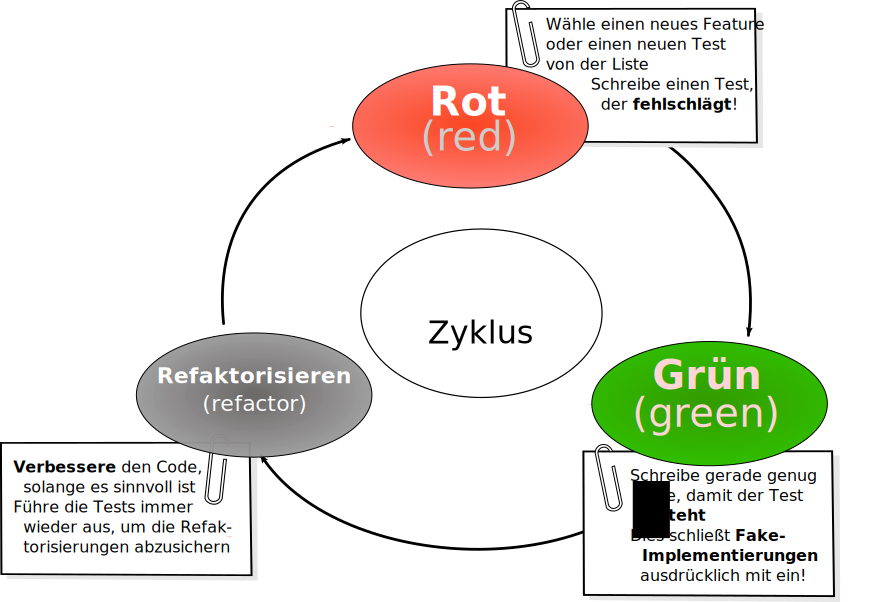
\includegraphics[width=0.85\textwidth]{./diagrams/red-green-refactor.pdf}
 % red-green-refactor.png: 884x602 pixel, 90dpi, 24.95x16.99 cm, bb=
 \caption{Red-Green-Refactor: Der TDD Entwicklungszyklus}
 
 \imgsource{Bildquelle: Der Autor}
 \label{fig:redgreenrefactor}
\end{figure}
  Im Detail sind das also folgende Phasen, vgl. Abbildung \ref{fig:redgreenrefactor}:
  \begin{enumerate}
   \item Schreibe einen neuen \glossar{test}. Dies kann der erste eines neuen Features sein, oder aber ein Test, um Funktionalität zum aktuellen Feature hinzuzufügen
   \item \textbf{Red}: Führe alle Tests aus, um sicherzugehen, dass der Test fehlschlägt. Andernfalls ist der Test überflüssig.
   \item \textbf{Green}: Nachdem der Test fehlschlägt, implementiere nun den einfachsten Code, damit der Test besteht\\
   Dies kann ausdrücklich auch eine Fake-Implementierung sein, also z.B. die Rückgabe eines konstanten Wertes anstelle einer Berechnung. Wichtig ist, dass diese Phase so schnell wie möglich verlassen wird.
   \item \textbf{Refactor}: Nachdem der Test bestanden wird, folgt nun die \textbf{wichtigste Phase}, die Refaktorisierungsphase.\\
   Da wir bereits einen Test haben, der unser gewünschtes Systemverhalten widerspiegelt, können wir gefahrlos \glossar{refaktorisieren}, d.h. meist Duplikation eliminieren. In dieser Phase findet das Design des Codes statt. Man macht sich Gedanken, wie die vorhanden Klassen optimal refaktorisiert werden können, um \glossarpl{smell} zu eliminieren, und welches Entwurfsmuster ggf. angewendet werden kann.
  \end{enumerate}
  
  
  Ein genau spezifizierter Ablauf ist in Abbildung \ref{fig:tddflow} zu finden. Auch dort ist zu sehen, dass die Testerstellungs und Refaktorisierungsphase strikt getrennt sind. Innerhalb ersterer solle nur möglichst schnell ein funktionierender Test erstellt und zum Bestehen gebracht werden. Die eigentliche Arbeit findet dann innerhalb der Refaktorisierungsphase statt, in der die wahrscheinlich suboptimale Implementierung verbessert wird, indem iterativ Design hinzugefügt wird.
  \begin{figure}[hp]
 \centering
 \includegraphics[width=0.75\textwidth]{./diagrams/tdd-flowchart.pdf}
 % tdd-flowchart.pdf: 510x1017 pixel, 72dpi, 17.99x35.88 cm, bb=0 0 510 1017
 \caption{Flussdiagram für TDD}
 \label{fig:tddflow}
 \imgsource{Bildquelle: Der Author}
\end{figure}


  Jeder Unittest soll prinzipiell nur eine Eigenschaft testen, die Entwicklung erfolgt also in kleinen Schritten. Dies hat direkte Auswirkungen auf die zu entwickelnden Objekte und Methoden, die ebenfalls übersichtlich werden sollen, und somit dem Objektbegriff, eine Klasse für eine Aufgabe, gerecht werden.
  
    \begin{figure}[hbtp]
 \centering
 \includegraphics[width=\textwidth]{./diagrams/ablauf.png}
 % ablauf.png: 955x263 pixel, 96dpi, 25.26x6.96 cm, bb=0 0 716 197
 \caption{Entwicklungsablauf}
 \caption*{(a) Traditionelle Entwicklung,  b) Testgetriebene Entwicklung}
 \imgsource{Quelle: \citep{janzen_does_2008}}
 \label{fig:devflow}
\end{figure}
\borderquote{It's about the design, not the tests.}{Kent Beck}
  Aus der Sicht des gesamten Entwicklungsprozesses wird somit die klassische Design-Phase in die Implementation eingegliedert. In Abbildung \ref{fig:devflow} wird der klassische Entwickungsablauf dem Ablauf bei einem TDD-orientierten Ablauf verglichen. Demnach wird die (Fein-)Design Phase scheinbar aus dem Ablauf entfernt, und findet sich als Refaktorisierungsphase wieder. Wichtig zu bemerken ist außerdem, dass TDD keineswegs auf eine Analysephase/einen Grobentwurf oder finale (System)-Tests verzichtet, sondern nachwievor auf diese angewiesen ist. 
  


  
  \subsection{Sonderfälle}
  \label{sec:tddspecialcircumstances}
  
  Der oben gezeigt Ablauf ist für den Normalfall, dem Entwickeln eines neuen Features gedacht. Für einige gesonderte Problemstellungen im Programmieralltag existieren ebenso gewisse Abläufe.
  
  \paragraph{Fehlerbehebung} Falls trotz der Verwendung von \glossar{TDD} Fehler in der Software gefunden werden, so erfolgt:
  \begin{enumerate}
   \item Schreibe einen Test, der den Fehler auslöst bzw. nachbildet
   \item Behebe den Fehler im Programmcode
   \item Führe alle Tests aus
  \end{enumerate}.
  Somit wird sichergestellt, das jeder bisher gefundene Fehler durch einen Test abgesichert wird.
  \paragraph{Spikes oder Spike Solution} In einigen Fällen ist es nicht ratsam, sofort mit einer testgetriebenen Entwicklung zu beginnen. Gerade wenn Prototypisierung, d.h. schnelle, erforschende, explorative Entwicklung mit dem ausschließlichen Ziel schnell ein lauffähiges Ergebnis zu erhalten gewünscht ist, dann kann auf Tests verzichtet werden. Eine solches, isoliert entwickeltes Experiment wird im \glossar{TDD}-Jargon "`Spike"' (zu deutsch: Spitze, Nadel) genannt. Die Idee dahinter ist es zu Lernen, und der produzierte Code wird i.d.R. gelöscht und nach dem Lernprozess nach originärer TDD-Manier entwickelt. Dies soll auch die gewählte Metapher einer Nadel aufzeigen: Schnell eine Nadel durch ein Brett bringen \citep{shore_art_2007}. Ausführliche Informationen über das Wann und Wie eines Einsatzes von Spikes finden sie in dem Buch "`The Art of Agile Development"' \citep{shore_art_2007}. Der Autor hat sogar das betreffende Kapitel online verfügbar gemacht\footnote{\url{http://jamesshore.com/Agile-Book/spike_solutions.html}}.

  \paragraph{Testen von privaten Methoden/Attributen} Da die objektorienterte Modellierung das Konzept des Information Hiding und Kapselung vorsieht, soll der interne Aufbau einer Klasse nach außen nicht sichtbar sein. Da Tests aber von außen auf eine Klasse zugreifen, stellt dies ein Problem dar. In einigen Sprachen löst man sich dieses Problem mittels Reflections, um über Umwege auf private Felder zuzugreifen. Dies spielt allerdings nur für das nachträgliche Testen von Legacy-Anwendungen eine Rolle. TDD in der Reinform betrieben habe niemals spezfische Tests von privaten Methoden oder Feldern, da diese ausschließlich durch Refaktorisierung enstanden sein könnten \citep{caroli_agile_2008}.
 % http://agiletips.blogspot.com/2008/11/testing-private-methods-tdd-and-test.html 
 
  
  
\subsection{Studien zu den Auswirkungen von TDD}

Viele Studien belegen die positiven Effekte, die \glossar{TDD} für die Software-Entwicklung hat.

% Code Qualität

So zeigt eine Fallstudie, dass TDD zu größerer Produktqualität bei gleichzeitigt hoher Flexibilität führt, was ebenso in einer höheren Zufriedenheit bei den Programmiern führt \citep{hans_wasmus_evaluation_2007}.


\marginnote{Empirische Untersuchung der Auswirkung auf Code-Qualität}Einer empirischen Studie von \citeauthor{madeyski_test-driven_2009} zufolge, sei TDD schwierg zu erlernen und in einigen Metriken (Klassen pro Methode, Development Speed, Anteil der bestandenen Akzeptanztests) nicht signifikant besser als traditionelle Test-Last-Methoden. Allerdings hatten die beteiligten TDD-geführten Projekte eine signifikant bessere Testabdeckung und geringere Kopplung unter den Klassen. Test-First sei letztendlich eine mächtige aber kontraintuitive Technik \citep{madeyski_test-driven_2009}.


In dem Artikel des IEEE-Software-Journals stellen \citeauthor{janzen_does_2008} eine Studie vor, die akademische und industrielle Javaprojekte die testgetrieben durchgeführt wurden (Test-First), mit denen, bei denen hinterher getestet wurde (Test-Last), vergleicht. Demnach zeigen die Ergebnisse an, dass Programmierer, die einen Test-First Ansatz verfolgen, tendenziell Software in kleineren Einheiten die weniger komplex sind, schreiben, als solche die erst nach der Entwicklung testen \citep{janzen_does_2008}.

\marginnote{Auswirkungen auf die Struktur -- Assignment Controllability}
Einer Studie von \citeauthor{mueller_effect_2006} zufolge, führt Testen im Allgemeinen zu weniger Methoden und geringerer Kopplung. Der Autor stellt auch eine potenzielle Metrik vor, um statistisch signifikant Projekte, die nach TDD betrieben wurden, von traditionellen Projekten zu unterscheiden: Assignment Controllability\footnote{Dies ist ein Maß, inwieweit der lokale Zustand einer Klasse/Methode von außen durch Parameter beeinflusst werden kann} \citep{mueller_effect_2006}. Allerdings rät der Autor zu weiteren Untersuchungen und setzt auch keinen Grenzwert an, ab welchem Grad der Controllability ein Projekt als TDD-Projekt bezeichnet werden kann.

% Verstaendnis
\marginnote{Verständnis von TDD in der Industrie}
Einer Umfrage unter 25 IT- und Entwicklungsleitern ergab, dass diese zwar die positiven Effekte unterstützen, aber nur 16\% TDD in der Praxis einsetzen, und nur 21\% Testvollständigkeit messen. Auch verstehen anscheinend etwa die Hälfte der Befragten den Begriff TDD falsch, nämlich als die reine Praxis Tests für alle denkbaren Problemfälle zu schreiben \citep{stelligent_inc_stelligent_2007}.

Das unter den Entwicklungsleitern der Fortune 500 Firmen, die von sich selbst behaupten, TDD zu betreiben, einige von Fehlannahmen ausgehen, wird in dem oben genannten Artikel genannt \citep{janzen_does_2008}. So setzen diese TDD mit automatisierten Tests gleich, oder behaupten sogar TDD sei das Schreiben ALLER Testfälle vor der Implementationsphase, anstelle der eigentlich gedachten kurzen Entwicklungs-Iterationen \citep{janzen_does_2008}.

% Auswirkungen auf Produktivit't und Bugs
\marginnote{Auswirkungen auf die Produktivität}
Einer Studie von Microsoft ergab, dass TDD-entwickelnde Teams eine 60\% -- 90\% geringere Fehlerdichte, aber eine 15\% -- 35\% längere Entwicklungszeit hätten, als nicht-TDD Entwickelnde \citep{nagappan_realizing_2008}.





  



\subsection{Prinzip des Emergent Design -- Evolutionäres Sofwaredesign}
Ein Konzept das TDD ermöglicht, ist das des sich Herausbildenden Designs. Gegenüber traditionellen Entwicklungsansätzen erfolgt die Entwicklungsphase (Design) hierbei nicht als eigenständige Phase, sondern ist streng in den Entwicklungsprozess integriert. Immer wenn ein Zyklus beim Refaktorisieren angelangt ist, findet effektiv Design statt. Eine Entwicklung nach TDD sucht den minimalsten Code, der die Anforderungen (Tests) erfüllt. Analog dazu, will ein Emergentes Design die kleinste Menge an benötigten Design suchen, im Gegensatz zu einem Software-Design, das im Vorfeld bedacht wurde. Durch die vielen Iterationen und die darausfolgenden zahlreichen Refaktorisierungen tritt nach und nach das Design hervor, welches optimal für das System ist. 



%discovering and harvesting patterns in existing Code

%GoF Patterns

%idiomatische Patterns: Patterns, die nur für genau eine Applikation oder innerhalb eines Unternehmens optimal sind. z.B. Security 
%technical patterns

%domain patterns -> common business patterns

%emergent -> discover this
%traditional design -> too early, Business Process can change way faster, speculation without facts
%Frameworks sollten nicht designt werden, sondern sich aus Code ergeben


%im Gegensatz zu einer Ingenieurswissenschaftlichen Tätigkeit, das ... -> Iterativ
% ward cummingham
%http://www.developerdotstar.com/mag/articles/reeves_design.html
%http://confreaks.net/videos/282-lsrc2010-real-software-engineering
%http://www.ibm.com/developerworks/java/library/j-eaed5/index.html

%because you think about every little component that goes into the system
%cheap to build, expensive to design
%BDUF (Big Design Upfront)


%http://www.thoughtworks.com/emergent-design

Einige Software-Architekten (\citeauthor*{neal_ford_emergent_2010}, \citeauthor*{jack_reeves_three_1992} und \citeauthor{glenn_vanderburg_real_2010}) proklamieren, dass praktisches Software-Engineering eigentlich keine ordinäre Ingenieursdisziplin sei. Ingenieure sind für die Planung und das Design verantwortlich, welches in aller Regel im Vorfeld der Implementierung stattfindet. Das klassische Software-Engineering empfindet diesen Prozess nach, was sich z.B. in dem Wasserfallmodell äußert. Diese Autoren äußern nun, dass dies für die meisten Softwareprojekte nicht ideal sei, da sich die Businessanforderungen meist im Laufe einer Entwicklung ändern. Traditionelles Softwaredesign abstrahiere zu früh und spekuliere ohne die letztendlichen Fakten zu kennen. Traditionelle Ingenieurswissenschaftliche Diszplinen hätten außerdem die Beschränkung, dass ein Build-Prozess äußerst teuer ist (man denke an Brücken oder Chips in Flugzeugsystemen), wohingegen dies bei Software in der Regel fast nichts koste. Dadurch kann die Software-Entwicklung ein iteratives Vorgehen nutzen \citep{neal_ford_emergent_2010}, \citep{glenn_vanderburg_real_2010}, \citep{jack_reeves_three_1992}. Statt eines großen Designs am Anfang (BDUF -- Big Design Upfront) soll das Design durch Entdeckung und Extrahieren aus dem Sourcecode gewonnen werden.

Abstraktion erfolgt beim Emergent Design durch Refaktorisieren, dem Anwendungen von Entwufsmustern und dem Anwenden von sogenannten \textbf{Idiomatischen Mustern} (Idomatic Patterns). Im Gegensatz zu den klassischen Entwufsmustern sind diese Muster nicht allgemein und für jedes Projekt anwendbar, sondern spezifisch für das Projekt, die Sprache oder das Unternehmen. Dies umfassen z.B. wie Transaktionen, Sicherheit und Infrastruktur verwendet wird. Viele Frameworks seien eine Sammlung von idomatischen Mustern für eine bestimmte Aufgabe, und viele gute Frameworks seien aus alltäglichen Problemlösungen hervorgegangen, u.a. auch \glossar{rails} \citep{neal_ford_ibm_2010}.

Ein Emergent Design kann auch ohne TDD in evolutionären Entwicklungsprozessen verwendet werden. Allerdings ist die Umsetzung ohne das Vorhandensein einer guten Test-Suite ein risikoreiches Unterfangen.
Mit seiner iterativen Herangehensweise passen Emergent Design in Kombination mit TDD dagegen perfekt in den Entwicklungszyklus der Agilen Software Entwicklung.


\subsection{Varianten}
\subsubsection{ATDD -- Acceptance TDD}
\label{sec:attd}

Die Akzeptanztest-getriebene Entwicklung ist eine Modifikation von \glossar{TDD}. Statt der Unittests, stehen hier die Akzeptanztests im Vordergrund
  
Das ganze lässt sich auch in den übergeordneten Prozess zum Entwickeln eines Features einordnen.
  %TODO RSPEC Buch macht das vor, Noch mal schauen, evtl alles Käse was ich hier geschrieben habe
\begin{enumerate}
 \item Schreibe einen Akzeptanztest/Systemtest um das aktuelle Feature zu implementieren
 \item Implementiere die Teilschritte, die notwendig sind, um den Akzeptanztest bestehen zu lassen. Verfahre bei der Implementation nach dem TDD Schema zur Implementierung der benötigten Units wie oben.
  \begin{enumerate}
   \item Schreibe einen Unittest
   \item Prüfe, ob der Test fehlschlägt, andernfalls zurück zu 1.
   \item Implementiere mit so wenig wie Code möglich, so dass der Test besteht
   \item Refaktorisiere
  \end{enumerate}
 \item Nachdem der Akzeptanztest besteht, Prüfe etwaige Refaktorisierungen für die Anwendungsebene.   
\end{enumerate}
  
Somit werden 2 Testebenen erstellt, die Akzeptanz- und die Unittests.


\subsubsection{Behavior Driven Development}
  
Die Behavior-Driven-Development ist eine Variation der Testgetriebenen Entwicklung, die die Kommunikation mit dem Kunden priorisiert. Sie sucht ein gemeinsames Vokabular für Business und Technologieinteressen.
  
Während bei klassischen Unit-Tests, und damit auch bei TDD, die Begriffe  "`Zusicherungen"' (assertions) und "`Tests"' beinhaltet, so hat BDD stattdessen "`Erwartungen"' (expectations) und "`Spezifikationen"' (specs/specifiations), und verwendet oft das Modalverb "`sollte"' (should).
  
\subsubsection{Design Driven Testing}
Design Driven Testing soll eine Umkehrung von Testgetriebener Software sein und wird Stephens und Rosenberg als Alternative dazu vorgeschlagen \citep{stephens_design_2010}. Sie kritisieren, dass TDD in Reinform betrieben, lediglich Unittests, aber keine Dokumentation oder höhere Tests höherer Levels produziert. Weiterhin monieren sie, dass TDD zu schwierig und aufwändig sei. Sie schlagen vor, stattdessen die Tests durch das Software-Design steuern zu lassen und sich auf komplexe Code-Abschnitte zu konzentrieren, anstatt wirklich jeden Code durch einen vorausgegangen Test entstehen zu lassen. Sie proklamieren die Nutzung von Akzeptanz- anstelle der Unittests. Code-Qualität soll durch ein gründliches vorheriges Design anstelle nachträglicher massiver Refaktorisierungen bewerkstelligt werden.
DDT eignet sich für größere Teams, da Wert auf manuelle Tests gelegt wird und z.B. ein QA-Team eingebunden wird. Da das Projektteam von it-jobs-und-stellen.de ein sehr kleines ist, wird auf diesen Entwicklungsprozess nicht näher eingegangen.

\newpage\section{Die Programmiersprache Ruby}

Ruby ist eine Programmiersprache, die von 1993 von Yukihiro Matsumoto bis heute entwickelt wurde. Dabei ließ er sich von seinen Lieblingsprogrammiersprachen Perl, Smalltalk, Eiffel, Ada und Lisp inspirieren, um eine neue Programmiersprache zu entwickeln, die sowohl funktionale, objektorientierte als auch prozedurale Programmierung ermöglicht \citep{ruby_visual_identity_team_about_2011}. 

Eine vollständige Einführung in Ruby zu geben würde den Rahmen dieser Diplomarbeit sprengen. Stattdessen wird ein Querschnitt durch die Sprache angelegt und die Hauptmerkmale und Unterschiede zu anderen Sprachen herausgestellt werden. Auch werden Auswirkungen auf das Testen diskutiert und mögliche Testwerkzeuge vorgestellt.

\subsection{Einführung in Ruby}
\marginline{\includegraphics[width=0.8\marginparwidth]{material/ruby.png}
Ruby ist eine Multiparadigma-Sprache}
Ruby ist eine interpretierte Sprache, auch Skriptsprache genannt. Dies bedeutet, dass der Programmcode zur Laufzeit analysiert und ausgeführt wird. Ruby ist auch eine Multiparadigma-Sprache, die Objektorientierung, prozedurale und funktionale Programmierung unterstützt.
\begin{description}
 \item[Prozedural] Funktionen und Variablen können außerhalb von Klassen definiert werden, in dem sogenannten \texttt{main}-Objekt
 \item[Objektorientierung] Alle Datentypen sind Objekte. Alle Variablen beinhalten Referenzen auf ein Objekt. Dies betrifft auch die primitiven Datentypen wie Integer und String
 \item[Funktional] Anonyme Funktionen und Closures sind Sprachbestandteil. Alle Statements haben einen Rückgabewert. Innerhalb einer Funktion ist dies immer das letzte Statement, falls kein expliziter Rücksprungpunkt gesetzt wurde
\end{description}


Das Ziel von Ruby ist es nicht (nur) maschinenlesbar zu sein, sondern vor allem die Lesbarkeit und Nutzbarkeit durch Menschen zu verbessern. Dies drückt sich durch eine Syntax aus, die oft laut als englische Sprache gelesen werden kann, und an vielen Stellen auf den Einsatz von Sonderzeichen verzichtet. So ist die Klammerung von Funktionsaufrufen optional, und kann weggelassen werden, solange die Zuordnung der Parameter eindeutig ist. Auch hält Ruby eine Vielzahl von redundanten Keywords bereit (Syntaktischer Zucker), um dem Programmierer mehrere Wege zur Lösung seines Problems zu ermöglichen.

\setlength{\epigraphwidth}{\marginparwidth}
\marginline{\epigraph{Ruby is simple in appearance, but is very complex inside, just like our human body}{Yukihiro Matsumoto}}
\setlength{\epigraphwidth}{0.8\textwidth}

Im Nachfolgenden sind einige Beispiele für die Verwendung von Ruby dargestellt, insbesondere die "`Alles ist ein Objekt"'-Philosophie.

 \begin{ruby}[label=Interaktive Ruby Sitzung (IRB)]
  \PY{g+gp}{>> }\PY{l+m+mi}{2}\PY{o}{.}\PY{n}{even?}
  \PY{g+go}{=> true}
  \PY{g+gp}{>> }\PY{l+s+s2}{"}\PY{l+s+s2}{hallo}\PY{l+s+s2}{"}\PY{o}{.}\PY{n}{upcase}
  \PY{g+go}{=> "HALLO"}
  \PY{g+gp}{>> }\PY{n+no}{Date}\PY{o}{.}\PY{n}{today} \PY{o}{+} \PY{l+m+mi}{2}
  \PY{g+go}{=> #<Date: 2011-06-30>}
  \PY{g+gp}{>> }\PY{n}{a} \PY{o}{=} \PY{l+m+mi}{4} \PY{o}{+} \PY{n+no}{Math}\PY{o}{.}\PY{n}{sqrt}\PY{p}{(}\PY{l+m+mi}{9}\PY{p}{)}
  \PY{g+go}{=> 7.0}
  \PY{g+gp}{>> }\PY{k}{if} \PY{p}{(}\PY{l+m+mi}{0}\PY{o}{.}\PY{n}{.}\PY{l+m+mi}{10}\PY{p}{)}\PY{o}{.}\PY{n}{include?} \PY{n}{a}
  \PY{g+gp}{>> }  \PY{n+nb}{puts} \PY{l+s+s2}{"}\PY{l+s+s2}{a liegt zwischen 0 und 10}\PY{l+s+s2}{"}
  \PY{g+gp}{>> }\PY{k}{end}
  \PY{g+go}{=> a liegt zwischen 0 und 10}
 \end{ruby}
\codecaption{Ruby Beispiele}

In den ersten beiden Beispielen sieht man, dass Integer und String Objekte sind, und über Instanzmethoden verfügen. Im ersten Beispiel wird geprüft, ob die Zahl gerade ist. Dabei existiert eine Konvention, dass boolsche Methoden mit einem Fragezeichen am Ende notiert werden. Im Dritten Beispiel wird eine Klassenmethode \texttt{today} auf die Klasse \texttt{Date} ausgeführt, welche ein Datumsobjekt konstruiert und zurückliefert. Da auch die Nutzung von Operatoren letzendlich nur syntaktischer Zucker für Methodenaufrufe sind, wird die Instanz-Methode \texttt{.+()} auf dieses Datums-Objekt ausgeführt, und liefert ein neues Datumsobjekt, welches zwei Tage in der Zukunft liegt.\\
Im Vierten Beispiel wird der Einsatz von Variablen demonstriert
Das letzte Beispiel zeigt den Einsatz von Kontrollstrukturen. Als Besonderheit seien hier auf den Ausdruck vom Typ \texttt{Range} \texttt{(0..10)} hingewiesen, der ein Intervall für den Integerzahlenbereich von 0 bis einschließlich 10 liefert. Die Methode \texttt{.include?(a)} testet nun, ob die Variable \texttt{a} in diesem Intervall liegt. Bei Eindeutigkeit können, wie oben bereits angesprochen, die Klammern eines Methodenaufrufes weggelassen werden.

Weiterhin erlaubt Ruby die Arbeit mit Lambdas, also anonymen Funktionen. Eine beliebte Verwendungsmöglichkeit ist die Bearbeitung von Arrays und listenähnlichen Strukturen.

% SNIPPET: [language=Ruby,label=Ruby Beispiel: Lambdas,caption=Ruby Beispiel: Lambdas]
% >> adder = lambda { |a,b|  a + b }                                                                                                         
% >> adder.call(1,2)                                                                                                                         
% => 3                                                                                                                                       
%                                                                                                                                            
% # Sortiere nach Standardvergleichsoperator                                                                                                 
% >> [4,5,7,3].sort()                                                                                                                        
% => [3, 4, 5, 7]                                                                                                                            
%                                                                                                                                            
% # Es kann auch eine benutzerdefinierte Sortierfunktion                                                                                     
% # angegeben werden                                                                                                                         
% >> [ "string",  "rails",  "ruby" ].sort_by{ |item| item.length }                                                                           
% => ["ruby", "rails", "string"]                                                                                                             
%                                                                                                                                            
% # Die Quadratzahlen von 1 bis 5                                                                                                            
% >> (1..5).map{|element| element * 2}                                                                                                       
% => [2, 4, 6, 8, 10]                                                                                                                        
%                                                                                                                                            

\begin{ruby}[label=IRB]
\PY{g+gp}{>> }\PY{n}{adder} \PY{o}{=} \PY{n+nb}{lambda} \PY{p}{\PYZob{}} \PY{o}{|}\PY{n}{a}\PY{p}{,}\PY{n}{b}\PY{o}{|}  \PY{n}{a} \PY{o}{+} \PY{n}{b} \PY{p}{\PYZcb{}}
\PY{g+gp}{>> }\PY{n}{adder}\PY{o}{.}\PY{n}{call}\PY{p}{(}\PY{l+m+mi}{1}\PY{p}{,}\PY{l+m+mi}{2}\PY{p}{)}
\PY{g+go}{=> 3}

\PY{g+go}{# Sortiere nach Standardvergleichsoperator}
\PY{g+gp}{>> }\PY{o}{[}\PY{l+m+mi}{4}\PY{p}{,}\PY{l+m+mi}{5}\PY{p}{,}\PY{l+m+mi}{7}\PY{p}{,}\PY{l+m+mi}{3}\PY{o}{]}\PY{o}{.}\PY{n}{sort}\PY{p}{(}\PY{p}{)}
\PY{g+go}{=> [3, 4, 5, 7]}

\PY{g+go}{# Es kann auch eine benutzerdefinierte Sortierfunktion}
\PY{g+go}{# angegeben werden}
\PY{g+gp}{>> }\PY{o}{[} \PY{l+s+s2}{"}\PY{l+s+s2}{string}\PY{l+s+s2}{"}\PY{p}{,}  \PY{l+s+s2}{"}\PY{l+s+s2}{rails}\PY{l+s+s2}{"}\PY{p}{,}  \PY{l+s+s2}{"}\PY{l+s+s2}{ruby}\PY{l+s+s2}{"} \PY{o}{]}\PY{o}{.}\PY{n}{sort\PYZus{}by}\PY{p}{\PYZob{}} \PY{o}{|}\PY{n}{item}\PY{o}{|} \PY{n}{item}\PY{o}{.}\PY{n}{length} \PY{p}{\PYZcb{}}
\PY{g+go}{=> ["ruby", "rails", "string"]}

\PY{g+go}{# Die Quadratzahlen von 1 bis 5}
\PY{g+gp}{>> }\PY{p}{(}\PY{l+m+mi}{1}\PY{o}{.}\PY{n}{.}\PY{l+m+mi}{5}\PY{p}{)}\PY{o}{.}\PY{n}{map}\PY{p}{\PYZob{}}\PY{o}{|}\PY{n}{element}\PY{o}{|} \PY{n}{element} \PY{o}{*} \PY{l+m+mi}{2}\PY{p}{\PYZcb{}}
\PY{g+go}{=> [2, 4, 6, 8, 10]}
\end{ruby}
\codecaption{Ruby Beispiel: Blöcke}
Das erste Beispiel zeigt, wie Funktionsausdrücke in Variablen gespeichert werden können, um später aufgerufen zu werden. Hier wird eine Addierfunktion definiert und aufgerufen.\\
Das Zweite Beispiel zeigt, wie Arrays verwendet werden, und durch eine bereits eingebaute Methode \texttt{sort} sortiert werden können. Falls die enthaltenen Objekte nicht trivial verglichen werden können, ermöglicht die Methode \texttt{sort\_by} des dritten Beispiels die Angabe einer benutzerdefinierten Sortierfunktion, hier z.B. die Sortierung nach der Länge eines Strings.\\
Im letzten Beispiel wird demonstriert, wie die Funktion \texttt{map} verwendet wird, die eine beliebige Funktion auf alle Elemente der Liste ausführt. Hier quadrieren wir alle Elemente unserer Liste und erhalten die quadrierte Liste als Rückgabewert von Map (Die originale Liste bleibt dabei unverändert).



\paragraph{Typ- und Objektsystem}
Wie schon erwähnt, sind bei Ruby alle Datentypen ein Objekt. Dies schließt insbesondere Klassen und primitive Datentypen mit ein, wie wir im folgenden Beispiel sehen können
% SNIPPET: 
% >> 2.class                                                                                                                                 
% => Fixnum                                                                                                                                  
% >> Fixnum.class                                                                                                                            
% => Class                                                                                                                                   
% >> Class.class                                                                                                                             
% => Class                                                                                                                                   
%                                                                                                                                            
% >> Fixnum.superclass                                                                                                                       
% => Integer                                                                                                                                 
% >> Fixnum.ancestors                                                                                                                        
% => [Fixnum, Integer, Precision, Numeric, Comparable, Object, Kernel]                                                                       
%                                                                                                                                            
\begin{ruby}[label=IRB]
\PY{g+gp}{>> }\PY{l+m+mi}{2}\PY{o}{.}\PY{n}{class} 
\PY{g+go}{=> Fixnum}
\PY{g+gp}{>> }\PY{n+no}{Fixnum}\PY{o}{.}\PY{n}{class} 
\PY{g+go}{=> Class}
\PY{g+gp}{>> }\PY{n+no}{Class}\PY{o}{.}\PY{n}{class} 
\PY{g+go}{=> Class}

\PY{g+gp}{>> }\PY{n+no}{Fixnum}\PY{o}{.}\PY{n}{superclass}
\PY{g+go}{=> Integer}
\PY{g+gp}{>> }\PY{n+no}{Fixnum}\PY{o}{.}\PY{n}{ancestors}
\PY{g+go}{=> [Fixnum, Integer, Precision, Numeric, Comparable, Object, Kernel]}
\end{ruby}
\codecaption{Klassenhierarchien}
% label{fig:f37300}

Das Literal \texttt{2} ist somit ein Objekt vom Typ \texttt{Fixnum}. Die Klasse Fixnum ist ihrerseits vom Typ \texttt{Class}. Da Ruby sowohl (Einfach-)Ableitungen als auch sogenannte Includes bzw. Mixins unterstützt, kann eine Klasse auch eine Menge von "`Vorfahren"' haben. Die gezeigte Klasse \texttt{Fixnum} verfügt somit standardmäßig sogar über 7 Oberklassen.

Ruby ist dynamisch stark typisiert. Das bedeutet, dass die Prüfung des Typs einer Variable zur Laufzeit stattfindet. Der Typ einer Variable ergibt sich damit aus ihrem aktuell beinhalteten Objekt. Durch die starke Typisierung ist es aber nicht möglich, invalide Operationen auf typ-inkompatible Objekte auszuführen, beispielsweise eine Addition von Integer mit String. Rubys Typsystem ist "`Duck-typed"', d.h. dass die Semantiken eines Objekts nicht durch seine Klasse und Ableitungshierarchie, sondern seine Methoden und Attributen bestimmt wird.\borderquote{"When I see a bird that walks like a duck and swims like a duck and quacks like a duck, I call that bird a duck."}{James Whitcomb Riley}

Ruby verfügt über lexikalische und dynamische Bindung\footnote{
\textbf{Static Scoping}: Variablen werden zur Compilezeit gebunden ohne den aufrufenden Code zu berücksichtigen\\
\textbf{Dynamic Scoping}: Variablen-Bindung kann nur im Moment der Ausführung des Codes festgestellt werden}, letztere wird allerdings seltener verwendet. Im der Basissyntax verwendet Ruby statische Bindung. Es existiert eine im Ruby-Core enthaltene Bibliothek \texttt{Dynamic} zum dynamischen binden, falls dies gewünscht sein sollte.


\paragraph{Reflektion und Introspection} Wichtig anzumerken sei noch, dass Klassen in Ruby nie geschlossen sind, sondern jederzeit erweitert werden können und vorhandene Methoden überschrieben werden können. So ist es z.B. möglich, die String-Klasse um eigene Funktionen zu erweitern. Ruby "`merkt"' sich allerdings die überschriebenen Methoden und ein Aufruf der überschriebenen Methoden ist stets mittels \texttt{super} möglich.

% SNIPPET: [language=Ruby,label=Ruby Beispiel offene Klassen,caption=Ruby Beispiel offene Klassen]
% >> class String                                                                                                                            
% >>   def remove_whitespace                                                                                                                 
% >>     self.gsub(/\s+/, "")                                                                                                                
% >>   end                                                                                                                                   
% >> end                                                                                                                                     
%                                                                                                                                            
% >> "Dies ist ein Test".remove_whitespace                                                                                                   
% => "DiesisteinTest"                                                                                                                        
%                                                                                                                                            
%                                                                                                                                         
\begin{ruby}[label=IRB]
\PY{g+gp}{>> }\PY{k}{class} \PY{n+nc}{String}
\PY{g+gp}{>> }  \PY{k}{def} \PY{n+nf}{remove\PYZus{}whitespace}
\PY{g+gp}{>> }    \PY{n+nb}{self}\PY{o}{.}\PY{n}{gsub}\PY{p}{(}\PY{l+s+sr}{/}\PY{l+s+sr}{\PYZbs{}}\PY{l+s+sr}{s+}\PY{l+s+sr}{/}\PY{p}{,} \PY{l+s+s2}{"}\PY{l+s+s2}{"}\PY{p}{)}
\PY{g+gp}{>> }  \PY{k}{end}
\PY{g+gp}{>> }\PY{k}{end}

\PY{g+gp}{>> }\PY{l+s+s2}{"}\PY{l+s+s2}{Dies ist ein Test}\PY{l+s+s2}{"}\PY{o}{.}\PY{n}{remove\PYZus{}whitespace}
\PY{g+go}{=> "DiesisteinTest"}
\end{ruby}
\codecaption{Ruby Beispiel offene Klassen}
% label{fig:9bf48b}

\paragraph{Generische Programmierung und Aspekte der Metaprogrammierung}
Metaprogrammierung umfasst die Analyse, Transformation und Generierung von Objektprogrammen durch Metaprogramme \citep{herrmann_2005}.  Sie ermöglicht es, Probleme effektiv zu lösen, die andernfalls nur mit erheblichem Aufwand, oder gar nicht zu lösen sind.\\
Ein beliebtes Idiom innerhalb der Ruby-Community ist es, verwendete Methoden auf Basis des Methodennamens zur Laufzeit zu erstellen (Generierung). Dies verwendet z.B. das beliebte \glossar{ORM}-Datenbankframework ActiveRecord, um einfache SQL-Statements anhand des Funktionsnamens zu erstellen (Ruby on Rails verwendet standardmäßig ActiveRecord als Schnittstelle zur Datenbank).
% SNIPPET: 
% >> Person.find_by_first_name("Stefan")                                                                                                     
% #  Person Load (0.2ms)  SELECT persons.* FROM persons                                                                                      
% #    WHERE users.first_name = 'Stefan' LIMIT 1       
\begin{ruby}[label=IRB]
\PY{g+gp}{>> }\PY{n+no}{Person}\PY{o}{.}\PY{n}{find\PYZus{}by\PYZus{}first\PYZus{}name}\PY{p}{(}\PY{l+s+s2}{"}\PY{l+s+s2}{Stefan}\PY{l+s+s2}{"}\PY{p}{)}
\PY{g+go}{#  Person Load (0.2ms)  SELECT persons.* FROM persons}
\PY{g+go}{#    WHERE users.first\PYZus{}name = 'Stefan' LIMIT 1}
\end{ruby}
\codecaption{Demonstration von generischen}
% label{fig:d0ee1e}


Die Methode \texttt{find\_by\_first\_name} existiert nicht, und wird zur Laufzeit auf Basis des Namens gebaut. Dies ist möglich, da Ruby sogennante Hooks (Callbacks) bereitstellt. Der Hook \texttt{ method\_missing} z.B., wird immer dann aufgerufen, wenn eine nicht-existierende Funktion aufgerufen wurde (wie in unserem Beispiel \texttt{find\_by\_first\_name}). Hier können wir nun die neue Methode auf Basis des gewünschten Funktionsnamens zur Laufzeit erstellen, oder andernfalls selbst eine Exception werfen. Ein weiterer Hook ist z.B. auch \texttt{method\_added}, der aufgerufen wird, wenn in einer Klasse eine Methode definiert wird\footnote{Einen guten Überblick über die Callbacks die Ruby bereitstellt, und was man damit kann, finden sie hier: \url{http://www.khelll.com/blog/ruby/ruby-callbacks/}}. Auf diese Weise sind z.B. die Modifikatoren \texttt{private} und \texttt{public} implementiert.

Ein weiteres Beispiel ist die Definition der relationalen Beziehungen zwischen den einzelnen Modellen innerhalb von \glossar{rails} (Ebenfalls unter der Verwendung von ActiveRecord).
\begin{ruby}[label=app/models/job.rb]
\PY{k}{class} \PY{n+nc}{Job} \PY{o}{<} \PY{n+no}{ActiveRecord}\PY{o}{::}\PY{n+no}{Base}
  \PY{n}{belongs\PYZus{}to} \PY{l+s+ss}{:user}
\PY{k}{end}
\end{ruby}
\codecaption{Nutzung von Metaprogrammierung zur Erstellung von Objektbeziehungen}
% label{fig:a7720a}

Hiermit definieren wir, dass ein Job einem User gehört, es also eine 1:N (oder 1:1)-Beziehung zwischen beiden gibt. Die dafür benötigten Getter und Setter werden mittels des Methodenaufrufs \texttt{belongs\_to} in die Klasse Job geschrieben.

Diese Beispiele sollten als kurzer Einstieg in Ruby dienen, und einen Querschnitt durch die Besonderheiten der Sprache aufzuzeigen.
Für eine weitere Vertiefung sei das Buch "`Programming Ruby 1.9"' empfohlen, das im Detail auf die neuste Version der Programmiersprache eingeht \citep{hunt_programming_2009}.



\subsection{Diskussion}

% Typunsicherheit, Geschwindigkeitsnachteil
\marginnote{Geschwindigkeitsverlust durch dynamische Typisierung}
Dynamisch-typisierte Sprachen, wie Ruby, haben gegenüber statisch-typisierten Sprachen einige Nachteile. Oft wird der Geschwindigkeitsnachteil angesprochen, den der Prozess des Interpretierens und die dynamische Typisierung verursachen. 
Der genaue Faktor variiert allerdings je nach Algorithmus und Implementierung, stark. Ein beliebter Benchmark, "`shootout.alioth"', vergleicht beliebte Algorithmen der Informatik, implementiert in verschiedenen Sprachen, miteinander. So ergibt sich z.B. in der Gegenüberstellung von Ruby mit C ein 4-fach bis 300-fach langsamere Ausführungszeit. Dem gegenüber steht allerdings nur die Hälfte bis $1/7$ der Menge an benötigtem Code \citep{computer_language_benchmarks_game_ruby_2011}. \\
Wichtig ist auch die verwendete Laufzeitumgebung. Neben der Referenzimplementierung von Matsumotu (Ruby MRI), existieren noch JRuby, eine Implementierung auf Basis der Java Virtuellen Maschine, und Rubinius. Die letzten beiden unterstützen auch eine sogenannte Just-in-time (JIT)-Kompilierung zur Verbesserung der Performanz bei längerer Ausführungszeit des Programms. Desweiteren gibt es gerade im Bereich Laufzeitoptimierung viel Bewegung innerhalb der Ruby-Implementierungen, und fast alle Ruby-Implementierungen nehmen stetig an Geschwindigkeit zu \citep{antonio_cangiano_great_2010}.

\marginnote{Fehlende Typsicherheit}
Allerdings bleiben Fehler, die der Compiler bereits entdeckt hätte, bis zur Ausführung oder schlimmstenfalls noch länger unentdeckt. Dazu gehören z.B. Tippfehler, bei denen der Wert einer nicht deklarierten Variable ausgelesen wird. Im Gegensatz zu z.B. PHP, wirft Ruby aber dann eine Exception.\\
Auf das Testen hat dies eine direkte Auswirkung. Viele Meinungen belegen, dass eine dynamisch typisierte Sprache mehr Tests benötigt, als eine statisch typisierte \citep{daniel_spiewak_dynamic_2010}. 


\marginnote{Vorteile aus der dynamischen Typisierung}
Ein Vorteil des Interpretierens, also der Übersetzung zur Laufzeit, ist eine hohe Plattformunabhängigkeit und ein leichterer Buildprozess, da das Kompilieren entfällt. 
Verfechter dynamischer Sprachen erklären weiterhin, dass diese sich ideal für prototypische Implementierungen eignen, da sich Anforderungen ständig ändern können. Weiterhin hätten Programme dynamischer Sprache eine potenziell hohe Wiederverwendbarkeit und eine höhere Lesbarkeit \citep{meijer_static_2005} \citep{ousterhout_scripting:_1998}.


% 
% All diese Methoden können, richtig angewendet, zur Verbesserung der Lesbarkeit der Programme, und damit zur Erhöhrung der Wartbarkeit, führen.
% 
% Auch das sehr beliebte Testframework Rspec, verwendet Metaprogrammierung, um Testfälle und Zusicherungen wie fast in der englischen Sprache zu formulieren. Dazu werden sämtliche Objekte von Ruby um Funktionen erweitert. Dies ist möglich, da die Klasse "`Objekt"', die Basisklasse (fast) aller Ruby-Klasse ist, um diese Methoden erweitert wurde.
% 

\paragraph{Schlussfolgerung}


\epigraph{Sometimes people jot down pseudo-code on paper. If that pseudo-code runs directly on their computers, it's best, isn't it? Ruby tries to be like that, like pseudo-code that runs. }{Yukihiro Matsumoto}
Die Verwendung von Ruby und anderen dynamischen Sprachen birgt durchaus Risiken, die zu beachten sind. Falls man sich dieser Risiken bewusst ist, und die Möglichkeiten der Sprache nutzt, um die Lesbarkeit zu verbessern, sind sie gerechtfertigt. Gerade bei der Entwicklung mit kleinen Entwicklerteams und Projekten mit engem Budget können dynamische Sprachen ihre Vorteile ausspielen, da sie eine schnellere Entwicklung ermöglichen. Im Gegensatz zu den meisten auf Syntax von C basierenden Sprachen (z.B. Java oder C\#), ist die Syntax von Ruby äußerst leserlich, da nur wenige Sonderzeichen verwendet werden. Auch ist Ruby sehr ausdrucksstark, weil die Deklaration entfällt und es viel sogenannten syntaktischen Zucker gibt. Alles dies kann, richtig angewendet, der Lesbarkeit zuträglich sein.



\subsection{Testframeworks für Ruby}
\subsubsection{Test::Unit und Minitest}
Test::Unit (Ruby 1.8.7) und Minitest (1.9.2) sind die Testbibliotheken, die Ruby standardmäßig mitbringt. Beide basieren auf dem xUnit-, bzw. SUnit-Design von Kent Beck, und sind für Nutzer von z.B. JUnit oder NUnit leicht nachvollziehbar. 

Für eine zu testende Klasse wird analoge eine Testklasse erstellt. Diese trägt per Definition denselben Namen wie die zu testende Klasse mit einem \texttt{Test} am Anfang. Um z.B. eine Klasse \texttt{Job} zu testen, wird eine Datei \texttt{job\_test.rb}  erstellt. Dort wiederrum wird eine Klasse mit Namen \texttt{TestJob} definiert. 

Eine solche Testklasse kann wie folgt aussehen:
% \begin{lstlisting}[language=Ruby,label=,caption=]
\begin{ruby}[label=Testen mit Test::Unit]
\PY{o}{[}\PY{n}{language}\PY{o}{=}\PY{n+no}{Ruby}\PY{p}{,}\PY{n}{label}\PY{o}{=}\PY{n+no}{Testen} \PY{n}{mit} \PY{n+no}{Test}\PY{o}{::}\PY{n+no}{Unit}\PY{p}{,}\PY{n}{caption}\PY{o}{=}\PY{n+no}{Testen} \PY{n}{mit} \PY{n+no}{Test}\PY{o}{::}\PY{n+no}{Unit} \PY{k}{in} \PY{n+no}{Ruby}\PY{o}{]}
\PY{n+nb}{require} \PY{l+s+s2}{"}\PY{l+s+s2}{job}\PY{l+s+s2}{"}

\PY{k}{class} \PY{n+nc}{TestJob} \PY{o}{<} \PY{n+no}{Test}\PY{o}{::}\PY{n+no}{Unit}\PY{o}{::}\PY{n+no}{TestCase}
  \PY{k}{def} \PY{n+nf}{setup}
    \PY{n+nv+vi}{@job} \PY{o}{=} \PY{n+no}{Job}\PY{o}{.}\PY{n}{create}
  \PY{k}{end}
  
  \PY{k}{def} \PY{n+nf}{teardown}
    \PY{n+no}{Job}\PY{o}{.}\PY{n}{delete\PYZus{}all}
  \PY{k}{end}
  
  \PY{k}{def} \PY{n+nf}{test\PYZus{}job\PYZus{}exists}
    \PY{n+nv+vi}{@job}\PY{o}{.}\PY{n}{title} \PY{o}{=}  \PY{l+s+s2}{"}\PY{l+s+s2}{Ruby on Rails in Entwickler}\PY{l+s+s2}{"}
    \PY{n+nv+vi}{@job}\PY{o}{.}\PY{n}{add\PYZus{}location\PYZus{}to\PYZus{}title}\PY{p}{(} \PY{l+s+s2}{"}\PY{l+s+s2}{Dresden}\PY{l+s+s2}{"}\PY{p}{)}
    
    \PY{n}{assert\PYZus{}equal}\PY{p}{(} \PY{l+s+s2}{"}\PY{l+s+s2}{Ruby on Rails Entwickler in Dresden}\PY{l+s+s2}{"}\PY{p}{,}  \PY{n+no}{Job}\PY{o}{.}\PY{n}{first}\PY{o}{.}\PY{n}{title}\PY{p}{)}
  \PY{k}{end}
\PY{k}{end}
\end{ruby}
\codecaption{Testen mit Test::Unit in Ruby}

Unsere Klasse \texttt{TestJob} erbt von der TestUnit-Basisklasse. Sie beinhaltet die besonderen Methoden \texttt{setup} und \texttt{teardown}, die jeweils vor, bzw. nach jedem einzelnen Testfall aufgerufen werden.
In der Setup-Methode nehmen wir z.B. das Anlegen eines Jobs vor, in der Teardown Methode löschen wir alle Jobs in der Datenbank, um einen sauberen Test zu gewährleisten (Isolation).

Danach können nun beliebig viele Testmethoden folgen, deren Namen mit \texttt{test\_} beginnen müssen.
Jede Testmethode besteht in der Regel aus einer Initialisierung (kann in die setup-Methode ausgelagert werden), der Ausführung einer zu testenden Aktion und dem Prüfen der danach geltenden Eigenschaften mittels Assertions. Assertions, also zu Deutsch Zusicherungen, sind vom Testframework bereitgestellt Funktionen, die übergebene Parameter auf gewisse Eigenschaften testen und daraus einen Testerfolg oder Fehlschlag ableiten. Sollte eine Assertion innerhalb eines Tests fehlschlagen, so gilt der gesamte Testfall als fehlgeschlagen. \\
Einige dieser Zusicherungen sind z.B.:
\begin{description}
 \item[assert(statement)] Prüft, ob der angegebene Ausdruck wahr ist (In Ruby sind alle Ausdrücke, außer \texttt{false} und \texttt{nil} wahr)
 \item[assert\_equal(expected, actually)] prüft, ob die beiden Statements gleich sind, hinsichtlich des \texttt{==}-Operators\footnote{Viele eingebaute Klassen prüfen auf Strukturgleichheit. Eigene Objekte werden ansonsten auf Adressengleichheit getestet. Man kann allerdings eine eigene Vergleichsoperation durch die Implementation der Instanzmethode \texttt{.==()} definieren}
 
 \item[assert\_raise(exception, \&block)] Prüft, ob innerhalb des übergebenen Codeblocks eine Exception vom Typ exception geworfen wird
 \item[assert\_match(regexp, string)] Prüft, dass der Ausdruck vom Typ String dem spezifizierten regulären Ausdruck matcht
\end{description}
%TODO Mehr Assertions und konkreter erklaeren, was sind a und b. Semantik: Falls Eingabe gleich (was bedeutet gleichheit)
Natürlich lassen sich beliebige weitere Zusicherungen definieren. \glossar{rails} z.B. definiert Zusicherungen, um zu testen, ob ein Objekt eine gültige Instanz hinsichtlich der definierten Validierungen ist (zum Thema Validierungen später mehr).

\paragraph{Testdatengenerierung}
Nachdem Testdaten einmal in zentraler Form definiert wurden, erledigt \glossar{rails} das Management, d.h. Laden und Löschen dieser, selbständig. Diese Art der Testdatenbereitstellung wird bei Rails als \textbf{Fixtures} bezeichnet. Rails setzt selbstständig die Datenbank nach jedem einzelnen Test zurück, oder kapselt die Tests innerhalb von Transaktionen, insofern die verwendete Datenbank dies unterstützt.
%TODO Abschnitt ueberarbeiten 
%TODO Wie macht man Testdaten? Wie waehlt man die Aus? muss in ein anderes Kapitel denke ich
% laedt definierte Objekte, andere Eigenschaften??  Wie waehlt man Testdaten aus??
% Globale Daten -> schlecht

Zur Generierung von größeren Mengen an zufälligen Daten einer bestimmten Domän (z.B. für Stresstests) existieren ebenfalls Lösungen. Mittels der \glossarpl{gem} "`populator"' und "`faker"' lassen sich beispielsweise eine beliebige Menge an gültig-anscheinenden Personendaten (Name, Vorname, Adresse, E-Mail-Adresse, Passwort,...) oder Blind-Texten generieren\footnote{Eine sehr gute Erklärung der Nutzung ist im Railscast \#128 zu finden \url{http://railscasts.com/episodes/126-populating-a-database}}.


\subsubsection{Cucumber}
\label{sec:cucumber}
Cucumber ist ein relativ neues Framework (2008), um mittels einer domainspezifischen Sprache verständliche automatisierte Tests zu schreiben. Dabei gibt es 2 Ebenen: In der obersten werden Testschritte in Englisch, Deutsch oder einer anderen der mehr als 30 unterstützten Sprachen spezifiziert. In der darunterliegenden werden diese Schritte in echten Testcode implementiert. \\
Im Folgenden sei ein Trivialbeispiel einer Anwendung, die Addieren unterstützt gezeigt.
\lstinputlisting[label=Cucumber: Additionsfeature in Deutsch,caption=Cucumber: Additionsfeature in Deutsch]{listings/addition.feature}
%TODO SyntaxHL
Wenn man nun die Datei mittels Cucumber ausführt, so wird darauf hingewiesen, dass die Testschritte noch nicht implementiert sind.

Eine Beispielimplementation (ohne Verwendung einer GUI-Anwendung) der Testschritte wäre:
\lstinputlisting[label=Cucumber: Implementierung der Additionstestschritte in Ruby,caption=Cucumber: Implementierung der Additionstestschritte in Ruby]{listings/steps.rb}
%TODO SyntaxHL

Wie man sehen kann, werden die Testschritte über die definierten regulären Ausdrücke gematcht. Jeder Schritt kann nun eine beliebige Implementierung besitzen. Meist ist es entweder eine Initialisierung, eine Aktion oder eine Erwartung, ausgedrückt durch die Schlüsselwörter \texttt{Angenommen}, \texttt{Wenn} und \texttt{Dann}, bzw. \texttt{Given}, \texttt{When} und \texttt{Then} im englischen Originaldialekt. Die Einteilung in klare Testschritte fördert die Wiederverwendbarkeit der Testschritte in anderen Szenarien.

Der Vorteil von Cucumber ist nun, dass diese Feature-Datei zusammen mit dem Kunden durchgesprochen werden kann, und am Ende eine funktionale Validierung durchzuführen. \\ 
Cucumber ist von der Syntax so generisch, dass damit beliebige Anwendungen getestet werden, da keine Annahmen über die darunterliegende Implementierung der Testschritte gemacht wird. Eine Möglichkeit, besonders im Zusammenhang mit \glossar{rails}, ist das Testen von Webanwendungen. Dabei kann z.B. auch ein echter Browser automatisiert bzw. simuliert werden, um den Test so authentisch am echten Nutzungsprozess wie möglich zu orientieren. \\
Neben Ruby wird auch die Implementierung der Testschritte in JVM und .NET-Sprachen unterstützt.
\newpage\newpage

\section{Ruby on Rails}
\label{sec:rails}
\epigraph{Ruby on Rails is a breakthrough in lowering the barriers of entry to programming. Powerful web applications that formerly might have taken weeks or months to develop can be produced in a matter of days.}{Tim O'Reilly, Gründer von O'Reilly Media}


Für das Projekt IT-jobs-und-stellen.de soll das Webframework Ruby-on-Rails\index{Ruby-on-Rails} verwendet werden. Rails wurde 2004 von der Firma 37signals\footnote{\url{http://37signals.com/}} unter der Leitung von David Heinemeier Hansson entwickelt und erlangte seitdem eine wachsende Popularität. Rails inspirierte viele andere Frameworks, wie z.B. cakePHP, Symfony, Groovy on Grails und ASP.NET MVC\footnote{\url{http://de.wikipedia.org/wiki/Ruby_On_Rails\#Verwandte_Frameworks}}.
% \footnote{ Sowie weitere PHP-Frameworks -- \url{http://www.h3rald.com/articles/rails-inspired-php-frameworks/}}

\bordergraphic{material/rails.png}
Viele professionelle Websites, die meist als Startup begannen, setzen bis heute auf Rails\index{Ruby-on-Rails}. Darunter Github, eine sehr beliebte Community für OpenSource-Programmierer,  Groupon, das führenden Unternehmen bei Online-Gutscheinen, XING, eine deutsche Online\hyp{}Community für Business-Kontakte, aber auch nicht-StartUps z.B. Yellow Pages, die Gelben Seiten der USA \citep{ruby_on_rails_2011}. Viele bekannte Firmen nutzen Rails auch auf die eine oder andere Weise, z.B. zur Entwicklung ihrer internen Webanwendungen. Dazu gehören BBC, Cisco, IBM, Oracle, die NASA, Siemens oder Yahoo\footnote{Weitere Firmen: \url{http://www.workingwithrails.com/high-profile-organisations}}.

Im Folgenden werden die Grundprinzipien und -konzepte von Ruby on Rails\index{Ruby-on-Rails} näher erläutert.

\subsection{Konzepte von Rails}
\label{sec:railsconcepts}
Rails\index{Ruby-on-Rails} ist ein Applikationsframework für Webanwendungen und basiert auf dem \glossar{MVC} \glossar{patterns}, welches eine 3-Schichten-Architektur darstellt. Jede Schicht hat fest definierte Aufgaben und sie bilden bei Rails normalerweise zusammen ein Dreigespann, \textbf{Ressource} genannt. Im Folgenden werden die Schichten kurz erläutert und am Beispiel einer Ressource "`Job"' erklärt.
\begin{description}
 \item[Model] In Klassen dieser Schicht werden Zugriffe auf die Persistenzschicht vorgenommen. Meist geschieht dies durch Ausführung von SQL-Befehlen auf eine relationale Datenbank\index{Datenbank}. Innerhalb von Rails\index{Ruby-on-Rails} ist das Schreiben von SQL aber meist nicht notwendig, da das \glossar{ORM}-\textit{ActiveRecord\index{ActiveRecord}} häufig verwendete SQL-Befehle abstrahiert. Die Geschäftslogik soll per Definition zu großem Teil in dieser Schicht erfolgen.

 Für einen Job ist das ein Modell\index{Ruby-on-Rails!Modell}, welches die Datenbank\index{Datenbank}tabelle "`jobs"' anspricht und z.B. die Attribute "`titel"', "`datum"' und "`beschreibung"' besitzt. Dabei können auf diesem Level auch datenbankunabhängige Constraints, die \textbf{Validierung\index{Ruby-on-Rails!Validierung}en} definiert werden, z.B. dass ein Job nur dann gespeichert werden soll, wenn der Titel mindestens 20 Zeichen lang ist und das Datum mindestens das Heutige ist.
 \item[Controller\index{Ruby-on-Rails!Controller}] Klassen dieser Schicht beinhalten Methoden, die von außen per HTTP erreichbar sind. Diese Methoden kommunizieren mit den korrespondierenden Models und bestimmen, welche View\index{Ruby-on-Rails!View} im Einzelnen ausgeliefert wird. Weitere Funktionen eines Controllers sind Authentifizierung und Autorisierung\footnote{Authentifizierung: Wer ist der Nutzer?\\Autorisierung: Was darf der Nutzer?}.\\
 Standardmäßig stellt Rails\index{Ruby-on-Rails} die \glossar{CRUD}-Operationen bereit, welche in Form eines REST Schemas angesprochen werden (mehr zu REST später).
%  \footnote{Representational State Transfer die HTTP-Methoden GET, POST, PUT, DELETE werden in Kombination mit einem definierten URL-Schema direkt auf die Aktionen \texttt{Auflisten, Anzeigen, Bearbeiten, Löschen, neu anlegen} gemappt.
%  \url{http://en.wikipedia.org/wiki/Representational_State_Transfer}}
 \item[View\index{Ruby-on-Rails!View}] Eine View ist in der Regel ein Stück HTML-Code, welches einem Model zugeordnet ist, das dem Clienten bei einer bestimmten Aktion ausgeliefert wird. Neben HTML ist auch JavaScript\index{JavaScript} oder XML eine mögliche Auslieferungsform.\\
 Für den Job wären Beispiele für eine View\index{Ruby-on-Rails!View} die Auflistung aller Jobs, einen Job im Detail anzeigen sowie das Formular zum Anlegen und Bearbeiten eines Jobs.
\end{description}
% TODO Graphik konkretisieren auf /jobs/12
 \begin{figure}[h]
  \centering
  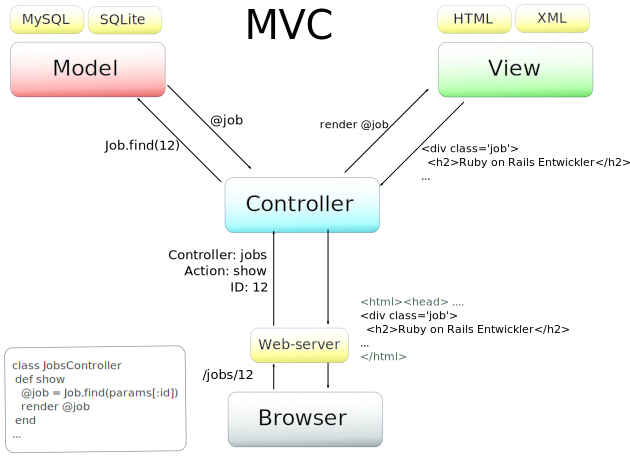
\includegraphics[width=0.7\textwidth]{./diagrams/mvc.pdf}
  % mvc-rails.png: 500x472 pixel, 72dpi, 17.64x16.65 cm, bb=
  % SOURCE
  \caption{MVC-Modell von Rails am Beispiel einer Anfrage /jobs/12}
  \label{fig:mvcrails}
\end{figure}
In Abbildung \ref{fig:mvcrails} ist der Ablauf einer Anfrage an den Server dargestellt. Die Anfrage des Browsers an die Website \texttt{http://localhost/jobs/12} wird über den Webserver, z.B. Apache2, an die Railsanwendung gestellt. Innerhalb von Rails wird dieser Anforderungsstring anhand der Routen, die die Anwendung anbietet, gematcht. In unserem Falle würde \texttt{/jobs/12} auf den Controller\index{Ruby-on-Rails!Controller} jobs aufgelöst werden. Innerhalb dieses Controllers wird eine Methode (Aktion) \texttt{show} erwartet.
Diese Methode wird nun ihrerseits eine Anfrage an das Model Job stellen, den Job mit der ID 12 aus der Datenbank\index{Datenbank} zu holen. Danach wird ein HTML-Template zur Detailanzeige des Jobs generiert.


Neben diesem architektonischen Konzept verfolgt Rails\index{Ruby-on-Rails} noch andere Strategien, um das Entwickeln produktiver zu gestalten.
\begin{description}
 \item[Convention over Configuration] Rails wurde konzipiert, um als Framework komplett out-of-the-box zu funktionieren. Außer der Datenbank\index{Datenbank}einstellung wird im Vorfeld keine Konfiguration benötigt. Diese Methodologie zieht sich auch durch das Ökosystem von Ruby\index{Ruby}. Die meisten externen Bibliotheken, bei Ruby \glossarpl{gem}\index{Gem} genannt, erschließen sich und funktionieren bereits binnen weniger Minuten. Dies macht das prototypische Entwickeln äußert effektiv. Weiterhin ist die Struktur eines Railsprojektes fest definiert. So gibt es u. a. einen Ordner \texttt{app} mit den Model-, Controller\index{Ruby-on-Rails!Controller}- und View\index{Ruby-on-Rails!View}-Dateien und einen Ordner \texttt{test}, der wiederum in \texttt{unit}, \texttt{functional}, \texttt{integration} und \texttt{performance} unterteilt ist. So finden sich Railsprogrammierer auch in fremden Projekten sofort zurecht.
 \item[Don't repeat yourself (DRY)] Hier ist das Ziel, die Duplikation soweit wie möglich zu reduzieren, um bei Änderungen nur an einer Stelle ansetzen zu müssen. Ein Beispiel ist die Definition der Attribute der Objekte durch das \glossar{ORM}. Im Gegensatz zu anderen ORM-Frameworks ist dies bei Rails\index{Ruby-on-Rails} nicht notwendig. Rails erstellt automatisch Getter und Setter für die in der Datenbank\index{Datenbank} definierten Tabellenspalten. Hintergrund ist, dass die Definition über Name und Typ der Attribute bereits in der Datenbank vorliegt und eine Wiederholung im Quellcode dem DRY-Prinzip widerspräche.
 \item[REST] Representational State Transfer ist eine Software-Architektur für HTTP-Web\hyp{}Services. Dabei werden neben den Standard-HTTP-Methoden GET und POST auch die selten benutzen Verben DELETE und PUT verwendet, um Aktionen auf eine Ressource zu definieren. Das Ziel ist ein sehr einfaches Design der URLs.

 Eine Verwendung der \glossar{CRUD}-Operationen mittels Rails\index{Ruby-on-Rails} würde am Beispiel einer Ressource \texttt{jobs} wie folgt aussehen:
  \begin{description}
  \item[GET /jobs.html] Auflisten aller Jobs, Ausgabe als HTML Format.
  \item[GET /jobs/12.xml] Job mit der ID 12 anzeigen, Formatiere als XML.
  \item[POST /jobs] Einen Job anlegen. Alle benötigten Parameter wie Titel, Beschreibung oder Datum sollten im POST-Body der HTTP-Anfrage enthalten sein.
  \item[PUT /jobs/12] Den Job mit der ID 12 aktualisieren. Die Eigenschaften, die aktualisiert werden, müssen als Parameter mit übergeben werden.
  \item[DELETE /jobs/12] Lösche den Job mit der ID 12.
  \end{description}
 Rails macht das Arbeiten im Kontext dieser Architektur sehr einfach und REST gilt als die bevorzugte Methode in der Community APIs\footnote{Application Programming Interface --  Eine Schnittstelle, um extern mit der Anwendung zu kommunizieren} zu erstellen.
 \item[Codegeneratoren] Rails bietet viele Codegeneratoren an, um schnell benötigte Klassen, Testfälle und Datenbanktabellen anzulegen.  Wie mit Hilfe der Codegeneratoren praktisch gearbeitet wird, wird später in Kapitel 7 dargelegt werden.
 \item[Full-Stack Webframework] Rails\index{Ruby-on-Rails} \borderquote{Rails will have strong defaults. They might change over time but Rails will remain opinionated.}{D. Hansson, Begründer von Rails}
bringt out-of-the-box alles mit, was zur Webentwicklung benötigt wird. Im Gegensatz zu anderen Webframeworks wurde für Datenbankanbindung\index{Datenbank}, Templatesystem, JavaScript-Framework\index{JavaScript}, Testframework und Webserver-API bereits eine Vorauswahl getroffen. Im aktuellen Rails 3.1 sind dies ActiveRecord\index{ActiveRecord} (Datenbank-Framework), ERB (Templating-Sprache), JQuery (JavaScript-Framework) sowie Test/Unit\index{Test/Unit-Framework} und Rack (Kommunikationsinterface für Komponenten). Die meisten dieser Komponenten lassen sich zwar leicht austauschen, Rails selbst aber behauptet "`opinionated"', also rechthaberisch / eigensinnig, zu sein und dem Entwickler Standards vorzugeben \citep{david_heinemeier_hansson_railsconf_2011}.

\end{description}

Eine komplette Einführung in die Programmierung mit Rails\index{Ruby-on-Rails} soll nicht Bestandteil dieser Diplomarbeit sein. Für eine weitere Einarbeitung seien die folgende Quellen empfohlen:
\begin{description}
 \item[Rails for Zombies] Dies ist ein moderner, interaktiver Onlinekurs. Greg Pollack und das Team von RailsEnvy verpackt die Lektionen in humorige interaktive Lernerfahrungen. Jeweils eingeleitet durch ein Video, muss der Teilnehmer Aufgaben direkt im Quelltext lösen. Die Teilnahme ist kostenlos.\\
 \url{http://railsforzombies.org/}
 \item[Agile Webdevelopment with Ruby on Rails] Das quasi-Standardwerk, u. a. geschrieben vom Rails-Begründer David Hansson. Das Buch wird meist parallel mit einer neuen Rails-Version in einer neuen Auflage gedruckt, aktuell die Dritte \citep{ruby_agile_2009}.
 \item[Rails Guides] Die von Ruby-on-Rails herausgegebenen "`Rails Guides"' sind eine gut strukturierte, kostenlose Online-Dokumentation, die nahezu alle Aspekte von Rails beleuchtet und anhand von praktischen Beispielen erläutert.\\
 \url{http://guides.rubyonrails.org/getting_started.html}
 \end{description}



\subsection{Diskussion}
Nach einem kurzen Überblick über Rails\index{Ruby-on-Rails} sollen nun die Eigenschaften des Frameworks sowie die sich daraus ergebenden Auswirkungen auf das Testen diskutiert werden.

\paragraph{Nachteile}

Oft wird angeführt,\randbem{Performanz} dass Ruby\index{Ruby} als Skriptsprache und Rails\index{Ruby-on-Rails} als darauf aufbauendes Framework eine schlechte Performanz besitzt und dadurch ungeeignet für große Webanwendungen ist.\\
Anderseits existieren Erfahrungen, dass eine clevere Architektur und Caching für skalierende Anwendung entscheidender ist als die letztendliche Ausführungszeit \citep{kirk_haines_ruby_2010}.
Dass eine Skalierung mit Rails\index{Ruby-on-Rails} möglich ist, zeigen z.B. Groupon, der führende Online-Coupon-Anbieter mit mehr als 50 Mio. Abonnenten und Twitter, die jeweils Rails verwenden bzw. verwendet haben \citep{ruby_on_rails_2011}.
%http://www.socialshopping.com/Groupon/news/Groupon-hits-50m-Subscribers-Shopping-site-sensation-201101210398/

 Da Rails\index{Ruby-on-Rails} ein komplettes Webframework ist,\randbem{Auswahl der Komponenten} wurden bei der Auswahl der einzelnen Komponenten bereits Entscheidungen getroffen.  Erst Anfang 2011 gab dazu es Kritik aus Teilen der Community, da ab der Version 3.1 "`CoffeeScript"' und "`SASS"' Bestandteil einer Rails-Distribution sind \citep{peter_cooper_rails_2011}. Beide sind Zwischensprachen, die in JavaScript\index{JavaScript} respektive CSS kompilieren und diese um Funktionalität erweitern. Allerdings kann jeder selbst wählen, ob er diese verwenden möchte.


Interaktion mit Legacy-Software ist nicht immer möglich. \randbem{Integration in bestehende Software}ActiveRecord\index{ActiveRecord} reserviert einige Spaltennamen, wie \texttt{type} und \texttt{class}. Eine Benennung der Spalten sollte der Ruby\index{Ruby}-Namenskonvention entsprechen, also nur Buchstaben, Zahlen und Unterstriche enthalten. Ansonsten können die Spalten nur über Umwege angesprochen werden. Rails\index{Ruby-on-Rails} ist äußerst effektiv, wenn man den gegebenen Konventionen folgt. Im Umkehrschluss bedeutet dies, dass man deutlich ineffektiver wird, wenn man die Konventionen von Rails ignoriert, z.B. wegen äußerer Umstände und Anforderungen.\\
Rails\index{Ruby-on-Rails} verzichtet auf die Verwendung von Constraints innerhalb der Datenbank\index{Datenbank}. In einigen Fällen, z.B. Bankensoftware, sind diese aber unbedingt erforderlich.

Ein Nachteil aus Sicht des Projektmanagement ist der Mangel\randbem{Mangel an Entwicklern} an freien Ruby-on-Rails\index{Ruby-on-Rails} Programmierern auf dem Arbeitsmarkt\footnote{z.B. \url{http://rubypays.blogspot.com/2011/04/rubyruby-on-rails-development-job.html}}. So kann bei einem langfristig angesetzten Projekt u. U. die Wartung nicht garantiert werden.

\paragraph{Vorteile}
Rails\index{Ruby-on-Rails} unterstützt den Software-Lebenszyklus,\randbem{Software\hyp{}Lebenszyklus} indem es von Haus aus drei Umgebungen definiert: Development, Test und Production. Diese unterscheiden sich in der Datenbank\index{Datenbank}, die sie benutzen, und Konfigurationsparametern zu Caching und Performanz. Weitere Umgebungen (z.B. Staging) können jederzeit definiert werden.


Dank der Modularität können als Persistenzgrundlage sowohl \randbem{Flexible Datenanbindung}relationale Datenbank\index{Datenbank}en wie MySQL, SQlite und Oracle, aber auch andere Formen wie NoSQL-Datenbanken transparent verwendet werden. Dank einer einfach zu verstehenden Syntax ist das Schreiben von SQL in vielen Fällen überflüssig und die Sicherheitslücke einer SQL-Injection wird ausgeschlossen. Bei relationalen Datenbanken verwendet ActiveRecord\index{ActiveRecord} standardmäßig Transaktionen, sofern die Datenbank dies unterstützt.



Rails\index{Ruby-on-Rails} bietet eine gute Ausgangsbasis, um sichere Websoftware zu entwickeln.\randbem{Sicherheit} Das Verwenden eines Datenbank\index{Datenbank}frameworks macht SQL-Injections unmöglich. \\
Cross-Site-Request-Forgery und Session-Angriffe werden erschwert, da Session und Cookie-Variablen standardmäßig verschlüsselt werden und bei Nutzung der Formulargeneratoren ein CSRF-Token generiert wird, um Replay-Angriffe zu unterbinden.

\borderquote{I needed to be way more productive...}{D. Hansson}
Die Codegeneratoren, die Aufteilung in \glossar{MVC} und die mitgelieferten Werkzeuge machen Rails\index{Ruby-on-Rails} äußerst produktiv und in wenigen Minuten lassen sich so bereits erste Anwendungen bauen. Der Begründer von Rails führte z.B. in einer Konferenz vor, wie man mit Rails ein Blog in 15 Minuten bauen könnte\footnote{http://media.rubyonrails.org/video/rubyonrails.mov}.


\paragraph{Testen mit Rails}
Rails\index{Ruby-on-Rails} bietet ausgezeichnete Voraussetzungen zum Softwaretest. Dafür spricht, dass...

\begin{itemize}
  \item benötigte Bibliotheken bereits mitgeliefert werden. Dies umfasst einen Test-Runner, vorkonfigurierte Test-Datenbanken (auf Basis von SQLite) und das Testframework Test/Unit,
  \item die Verwendung stark erleichtert wird, da Rails\index{Ruby-on-Rails} beim Nutzen der Codegeneratoren analoge Testdateien gleich mitgeneriert,
 \item neben den mitgelieferten Tools das Rails\index{Ruby-on-Rails}-Ökosystem eine Vielzahl von Testtools bereitstellt, u.a. Rspec (\glossar{BDD}-Testframework), Rcov (Testabdeckung\index{Test!Testabdeckung}), diverse Mock\index{Test-Double!Mock}bibliotheken (mocha, FlexMock, RR, Rspec Mocks), Tools zum Generieren und Bereitstellen von Testdaten\index{Test!Testdaten} (Fixtures, Factories, Faker) und \glossarpl{metrik}\index{Code-Metrik} (metric-fu).
 \item das Testen einen sehr hohen Stellenwert in der Ruby- und Rails-Comumnity hat. Nahezu alle namhaften Ruby-Programmierer schreiben umfassende Tests \citep{devries_rails_2008}. Das Resultat ist, dass auch fast alle \glossarpl{gem}\index{Gem} bei Ruby eine "`solid suite of tests"' haben \citep{devries_rails_2008}.
\end{itemize}

Rails\index{Ruby-on-Rails} unterstützt verschiedene Testarten out-of-the-box:
\begin{description}
 \item[Unittest\index{Test!Unittest}s] oder Modell\index{Ruby-on-Rails!Modell}tests (model test)\\
 Testziel: alle (komplexeren) Methoden, die das Modell\index{Ruby-on-Rails!Modell} anbietet, seine Validierung\index{Ruby-on-Rails!Validierung}en und Beziehungen zu anderen Objekten.
 \item[Funktionale Tests] Untersuchungsgegenstand sind die Controller\index{Ruby-on-Rails!Controller}. \\
 Testziel: Getestet wird meist der Arbeitsablauf innerhalb eines Controller\index{Ruby-on-Rails!Controller}s, also Weiterleitungen, Benachrichtigungen und welches Template gerendert wird.
 Damit können gleichzeitig auch View\index{Ruby-on-Rails!View}-Tests unternommen werden, also z.B. die Untersuchung, ob ein bestimmtes HTML-Element auf der Webseite zu sehen ist.
 \item[Integrationstests] Es wird ein Browser simuliert, der von außen auf die Applikation zugreift.\\
 Zielstellung: Testen komplexer Interaktionen zwischen verschiedenen Teilen der Software.\\
 Beispiel: Ein User loggt sich ein und legt einen neuen Job an.
 \item[Performanz-Tests] Eine Testart, die alle Methoden aus Unittest\index{Test!Unittest}s und funktionalen Tests beinhaltet.\\
 Zielstellung: Lokalisation von Performanz-Flaschenhälsen in allen Bereichen der Software. \\
 Beispiel: Es werden 1000 Jobs generiert und geprüft, ob die Anzeige schnell genug läuft.
\end{description}

\section{Testframeworks für Ruby}
\epigraph{Ruby has laid the way in having a test-infected culture around the language.}{Nathaniel Talbott (Entwickler von Test/Unit)}

Rails\index{Ruby-on-Rails} liefert standardmäßig das auf dem xUnit-Schema basierende Testframework Test/Unit\index{Test/Unit-Framework} mit. In der Version 1.9.x bringt Ruby\index{Ruby} das Testframework Minitest in der Standardbibliothek mit, welches ebenfalls Tests nach dem xUnit-Schema unterstützt. Darüber hinaus existieren zahllose weitere Testframeworks für Ruby. Eines für den Akzeptanztest\index{Akzeptanztest} ist Cucumber\index{Cucumber}, welches eine Business-readable \glossar{DSL}\footnote{Eine domänspezifische Sprache, die durch Kunden nachvollzogen werden kann. Siehe \url{http://martinfowler.com/bliki/BusinessReadableDSL.html}} für die Definition von Spezifikationen darstellt.
\subsection{Test/Unit}
\label{sec:rubyTestUnit}
Test/Unit\index{Test/Unit-Framwork} basiert auf dem xUnit-, bzw. SUnit-Design von Kent Beck und ist für Nutzer von z.B. JUnit oder NUnit leicht nachvollziehbar.

Für eine zu testende Klasse wird analog eine Testklasse erstellt. Diese trägt per Definition den selben Namen wie die zu testende Klasse mit einem \texttt{Test} am Anfang. Um z.B. eine Klasse \texttt{Job} zu testen, wird eine Datei \texttt{job\_test.rb}  erstellt. Dort wiederum wird eine Klasse mit Namen \texttt{TestJob} definiert.


Eine solche Testklasse kann wie folgt aussehen:
\begin{ruby}[label=Testen mit Test/Unit]
\PY{n+nb}{require} \PY{l+s+s2}{"}\PY{l+s+s2}{job}\PY{l+s+s2}{"}

\PY{k}{class} \PY{n+nc}{TestJob} \PY{o}{<} \PY{n+no}{Test}\PY{o}{::}\PY{n+no}{Unit}\PY{o}{::}\PY{n+no}{TestCase}
  \PY{k}{def} \PY{n+nf}{setup}
    \PY{n+nv+vi}{@job} \PY{o}{=} \PY{n+no}{Job}\PY{o}{.}\PY{n}{create}
  \PY{k}{end}

  \PY{k}{def} \PY{n+nf}{teardown}
    \PY{n+no}{Job}\PY{o}{.}\PY{n}{delete\PYZus{}all}
  \PY{k}{end}

  \PY{k}{def} \PY{n+nf}{test\PYZus{}job\PYZus{}exists}
    \PY{n+nv+vi}{@job}\PY{o}{.}\PY{n}{title} \PY{o}{=}  \PY{l+s+s2}{"}\PY{l+s+s2}{Ruby on Rails in Entwickler}\PY{l+s+s2}{"}
    \PY{n+nv+vi}{@job}\PY{o}{.}\PY{n}{save}

    \PY{n}{assert\PYZus{}equal}\PY{p}{(} \PY{l+s+s2}{"}\PY{l+s+s2}{Ruby on Rails Entwickler in Dresden}\PY{l+s+s2}{"}\PY{p}{,}  \PY{n+no}{Job}\PY{o}{.}\PY{n}{first}\PY{o}{.}\PY{n}{title}\PY{p}{)}
  \PY{k}{end}
\PY{k}{end}
\end{ruby}
\codecaption{Testen mit Test/Unit in Ruby}

Unsere Klasse \texttt{TestJob} erbt von der \texttt{TestUnit}-Basisklasse. Sie beinhaltet die besonderen Methoden \texttt{setup} und \texttt{teardown}, die jeweils vor bzw. nach jedem einzelnen Testfall\index{Test} aufgerufen werden.
In der \texttt{setup}-Methode nehmen wir z.B. das Anlegen eines Jobs vor, in der teardown-Methode löschen wir alle Jobs in der Datenbank\index{Datenbank}, um einen sauberen Test \index{Test}zu gewährleisten (Isolation).

Danach können nun beliebig viele Testmethoden folgen, deren Namen mit \texttt{test} beginnen müssen.
Jede Testmethode besteht in der Regel aus einer Initialisierung, der Ausführung einer zu testenden Aktion und dem Prüfen der danach geltenden Eigenschaften mittels \textbf{Assertions} (vgl. ebenfalls Abschnitt \ref{sec:testUnit}. Diese Assertions, also zu Deutsch "`Zusicherungen"', sind vom Testframework bereitgestellt Funktionen, die übergebene Parameter auf gewisse Eigenschaften testen und daraus einen Testerfolg oder Fehlschlag ableiten. Sollte eine Assertion innerhalb eines Tests fehlschlagen, so gilt der gesamte Testfall\index{Test} als fehlgeschlagen. \\
Einige dieser Zusicherungen sind z.B.:
\begin{description}
 \item[\texttt{assert(statement)}] Prüft, ob der angegebene Ausdruck wahr ist (In Ruby\index{Ruby} sind alle Ausdrücke außer \texttt{false} und \texttt{nil} wahr).
 \item[\texttt{assert\_equal(expected, actually)}] Prüft, ob die beiden Statements hinsichtlich des \texttt{==}-Operators gleich sind\footnote{Viele eingebaute Klassen prüfen auf Strukturgleichheit. Eigene Objekte werden ansonsten auf Adressengleichheit getestet. Man kann allerdings eine eigene Vergleichsoperation durch die Implementation der Instanzmethode \texttt{.==()} definieren}

 \item[\texttt{assert\_raise(exception, \&block)}] Prüft, ob innerhalb des übergebenen Codeblocks eine Exception vom Typ exception geworfen wird.
 \item[\texttt{assert\_match(regexp, string)}] Prüft, dass der Ausdruck vom Typ String mit dem spezifizierten regulären Ausdruck matcht.
\end{description}
Natürlich lassen sich beliebige weitere Zusicherungen definieren. \glossar{rails} z.B. definiert Zusicherungen um zu testen, ob ein Objekt eine gültige Instanz hinsichtlich der definierten Validierung\index{Ruby-on-Rails!Validierung}en ist (Validierungen wurden bereits im Abschnitt \ref{sec:railsconcepts} erläutert).

\paragraph{Testdatengenerierung}
Nachdem Testdaten\index{Test!Testdaten} (vgl. Abschnitt \ref{sec:test}) einmal in zentraler Form definiert wurden, erledigt \glossar{rails} das Management, d.h. Laden und Löschen dieser, selbständig. Diese Art der Testdatenbereitstellung wird bei Rails \textbf{Fixtures} bezeichnet. Rails setzt selbstständig die Datenbank\index{Datenbank} nach jedem einzelnen Test \index{Test}auf die Fixtures zurück oder kapselt die Tests innerhalb von Transaktionen, sofern die verwendete Datenbank dies unterstützt.\\
Allerdings ist diese Form der Testdaten\index{Test!Testdaten}bereitstellung nicht unumstritten. Fixtures sind globale Daten, die in jedem Test verfügbar sind, obwohl sie nur in wenigen Testfällen benötigt werden, und machen es schwierig, Grenzfälle effektiv zu definieren. Außerdem sind die Testdaten nicht in derselben Datei wie der Test zu finden, womit man Tests nur verstehen kann, wenn man die Fixtures kennt. Eine mögliche Lösung ist es, stattdessen \textbf{Factories}\footnote{http://www.dan-manges.com/blog/38} einzusetzen, die zentral Regeln definieren, wie valide Instanzen von Modell\index{Rails!Modell}en gebaut werden. Die Tests nutzen dann die Factory, um sich z.B. einen neuen Job generieren zu lassen und für den aktuellen Testfall verändern.

Zur Generierung von größeren Mengen an zufälligen Daten einer bestimmten Domäne (z.B. für Stresstests) existieren ebenfalls Lösungen. Mittels der \glossarpl{gem}\index{Gem} "`populator"' und "`faker"' lässt sich beispielsweise eine beliebige Menge an gültig erscheinenden Personendaten (Name, Vorname, Adresse, E-Mail-Adresse, Passwort, ...) oder Blindtexten generieren\footnote{Eine sehr gute Erklärung zur Nutzung beider Gems ist im Railscast \#128 zu finden \url{http://railscasts.com/episodes/126-populating-a-database}}.


\subsection{Cucumber}
\label{sec:cucumber}
Cucumber\index{Cucumber} ist ein relativ neues Framework (2008), um mittels einer domainspezifischen Sprache  (\glossar{DSL}) verständliche automatisierte Tests zu schreiben. Dabei gibt es 2 Ebenen: in der Oberen werden \textit{Testschritt\index{Cucumber!Testschritt}e} in Englisch, Deutsch oder einer anderen der mehr als 30 unterstützten Sprachen spezifiziert. In der darunter Liegenden werden diese Schritte in echtem Testcode implementiert. \\
Im Folgenden sei ein Trivialbeispiel einer Anwendung, die Addieren implementiert, gezeigt.
%\lstinputlisting[label=Cucumber: Additionsfeature in Deutsch,caption=Cucumber: Additionsfeature in Deutsch]{listings/addition.feature}
\begin{ruby}[label=features/addition.feature]
\PY{c}{# language: de}
\PY{n+nc}{Funktionalität}\PY{n+nc}{:}\PY{n+no}{ Addition zweier Zahlen}
\PY{n+nb}{ }\PY{n+nb}{ }\PY{n+nb}{H}\PY{n+nb}{i}\PY{n+nb}{e}\PY{n+nb}{r}\PY{n+nb}{ }\PY{n+nb}{w}\PY{n+nb}{ü}\PY{n+nb}{r}\PY{n+nb}{d}\PY{n+nb}{e}\PY{n+nb}{ }\PY{n+nb}{e}\PY{n+nb}{i}\PY{n+nb}{n}\PY{n+nb}{e}\PY{n+nb}{ }\PY{n+nb}{g}\PY{n+nb}{r}\PY{n+nb}{o}\PY{n+nb}{b}\PY{n+nb}{e}\PY{n+nb}{ }\PY{n+nb}{B}\PY{n+nb}{e}\PY{n+nb}{s}\PY{n+nb}{c}\PY{n+nb}{h}\PY{n+nb}{r}\PY{n+nb}{e}\PY{n+nb}{i}\PY{n+nb}{b}\PY{n+nb}{u}\PY{n+nb}{n}\PY{n+nb}{g}\PY{n+nb}{ }\PY{n+nb}{d}\PY{n+nb}{e}\PY{n+nb}{s}\PY{n+nb}{ }\PY{n+nb}{B}\PY{n+nb}{u}\PY{n+nb}{s}\PY{n+nb}{i}\PY{n+nb}{n}\PY{n+nb}{e}\PY{n+nb}{s}\PY{n+nb}{s}\PY{n+nb}{v}\PY{n+nb}{a}\PY{n+nb}{l}\PY{n+nb}{u}\PY{n+nb}{e}\PY{n+nb}{s}
\PY{n+nb}{ }\PY{n+nb}{ }\PY{n+nb}{u}\PY{n+nb}{n}\PY{n+nb}{d}\PY{n+nb}{ }\PY{n+nb}{d}\PY{n+nb}{e}\PY{n+nb}{r}\PY{n+nb}{ }\PY{n+nb}{R}\PY{n+nb}{a}\PY{n+nb}{h}\PY{n+nb}{m}\PY{n+nb}{e}\PY{n+nb}{n}\PY{n+nb}{b}\PY{n+nb}{e}\PY{n+nb}{d}\PY{n+nb}{i}\PY{n+nb}{n}\PY{n+nb}{g}\PY{n+nb}{u}\PY{n+nb}{n}\PY{n+nb}{g}\PY{n+nb}{e}\PY{n+nb}{n}\PY{n+nb}{ }\PY{n+nb}{s}\PY{n+nb}{t}\PY{n+nb}{e}\PY{n+nb}{h}\PY{n+nb}{e}\PY{n+nb}{n}
  \PY{n+nc}{Szenario}\PY{n+nc}{:}\PY{n+no}{ Addition von ganzen positiven Zahlen}
\PY{k}{    Wenn }ich \PY{l+s}{"}\PY{l+s}{1}\PY{l+s}{"} für a und \PY{l+s}{"}\PY{l+s}{2}\PY{l+s}{"} für b eingebe
    \PY{k}{Und }auf \PY{l+s}{"}\PY{l+s}{A}\PY{l+s}{d}\PY{l+s}{d}\PY{l+s}{i}\PY{l+s}{e}\PY{l+s}{r}\PY{l+s}{e}\PY{l+s}{n}\PY{l+s}{"} klicke
    \PY{k}{Dann }sehe ich \PY{l+s}{"}\PY{l+s}{3}\PY{l+s}{"}
\end{ruby}
\codecaption{Cucumber: Definition eines Additionsfeature (in Deutsch)}

Wenn man nun die Datei mittels Cucumber\index{Cucumber} ausführt, so wird darauf hingewiesen, dass die Testschritt\index{Cucumber!Testschritt}e noch nicht implementiert sind.

Eine Beispielimplementation (ohne Verwendung einer GUI-Anwendung) der Testschritt\index{Cucumber!Testschritt}e wäre:
\begin{ruby}[label=features/step\_definitions/steps.rb]
\PY{n+no}{Wenn}\PY{l+s+sr}{ /\PYZca{}}\PY{l+s+sr}{ich "([\PYZca{}"]*)" für a und "([\PYZca{}"]*)" für b eingebe\$}\PY{l+s+sr}{/} \PY{k}{do} \PY{o}{|}\PY{n}{arg1}\PY{p}{,} \PY{n}{arg2}\PY{o}{|}
  \PY{n+nv+vi}{@addierer} \PY{o}{=} \PY{n+no}{Addierer}\PY{o}{.}\PY{n}{new}\PY{p}{(}\PY{n}{arg1}\PY{p}{,} \PY{n}{arg2}\PY{p}{)}
\PY{k}{end}

\PY{n+no}{Wenn}\PY{l+s+sr}{ /\PYZca{}}\PY{l+s+sr}{auf "([\PYZca{}"]*)" klicke\$}\PY{l+s+sr}{/} \PY{k}{do} \PY{o}{|}\PY{n}{arg1}\PY{o}{|}
  \PY{n+nv+vi}{@result} \PY{o}{=} \PY{n+nv+vi}{@addierer}\PY{o}{.}\PY{n}{add}\PY{p}{(}\PY{p}{)}
\PY{k}{end}

\PY{n+no}{Dann}\PY{l+s+sr}{ /\PYZca{}}\PY{l+s+sr}{sehe ich "([\PYZca{}"]*)"\$}\PY{l+s+sr}{/} \PY{k}{do} \PY{o}{|}\PY{n}{arg1}\PY{o}{|}
  \PY{n}{assert\PYZus{}equal}\PY{p}{(} \PY{n}{arg1}\PY{o}{.}\PY{n}{to\PYZus{}f}\PY{p}{,} \PY{n+nv+vi}{@result}\PY{p}{)}
\PY{k}{end}

\end{ruby}
\codecaption{Cucumber: Implementierung der Additionstestschritte in Ruby}
Die Anweisungen\randbem{Funktionsweise} des Akzeptanztest\index{Akzeptanztest}s werden auf die definierten Testschritt\index{Cucumber!Testschritt}e gemappt, die Cucumber\index{Cucumber} dann sequentiell ausführt.
Jeder dieser Testschritt\index{Cucumber!Testschritt}e kann nun eine beliebige Implementierung besitzen. Meist ist es entweder eine Initialisierung, eine Aktion oder eine Erwartung, ausgedrückt durch die Schlüsselwörter \texttt{Angenommen}, \texttt{Wenn} und \texttt{Dann}, bzw. \texttt{Given}, \texttt{When} und \texttt{Then} im englischen Originaldialekt. Die Einteilung in klare Testschritte fördert die Wiederverwendbarkeit der Testschritte in anderen Szenarien.

Der Vorteil von Cucumber\index{Cucumber} ist nun,\randbem{Vorteile für Kundenzusammenarbeit} dass diese Feature-Datei zusammen mit dem Kunden durchgesprochen werden kann und dass man damit an Ende eine funktionale Validierung gegenüber der Spezifikation automatisiert durchführen kann. \\
Die Syntax von Cucumber\index{Cucumber} ist so generisch, dass damit beliebige Anwendungen getestet werden können, da keine Annahmen über die darunterliegende Implementierung der Testschritt\index{Cucumber!Testschritt}e gemacht wird.
Neben Ruby\index{Ruby} wird auch die Implementierung der Testschritt\index{Cucumber!Testschritt}e in Java und C\# unterstützt.

\paragraph{Testen von Webanwendungen}
Eine Einsatzmöglichkeit von Cucumber\index{Cucumber}, besonders im Zusammenhang mit \glossar{rails}, ist das Testen von Webanwendungen. Dabei ist es üblich, einen Browser zu automatisieren\index{Browser!Automatisierter} bzw. simulieren (vgl. Abschnitt \ref{sec:acceptance}), um den Test \index{Test}so authentisch am echten Nutzungsprozess wie möglich zu orientieren.

Um unsere Tests von der Steuerung eines konkreten Browsers unabhängig zu machen, verwenden wir verschiedene Middlewares. Wir haben uns für Capybara\index{Capybara} entschieden, welches sehr flexibel bei der Wahl der Browser-Engine ist. Der eigentliche Test, d.h. die Auswertung der Zusicherung kann durch ein beliebiges Testframework durchgeführt werden; in unserem Falle wieder mit Test/Unit\index{Test/Unit-Framwork}. Durch Capybara haben wir nun die Möglichkeit, zwischen einem simulierten Browser\index{Browser!Simulierter} (z.B. \textbf{\glossar{racktest}}) und automatisierten Browsern\index{Browser!Automatisierter} (Firefox, Chrome, etc. durch eine weitere Middleware, Selenium\index{Selenium}) je nach Bedarf ohne große Änderungen am Testcode zu wechseln.
\begin{figure}[htbp]
 \centering
 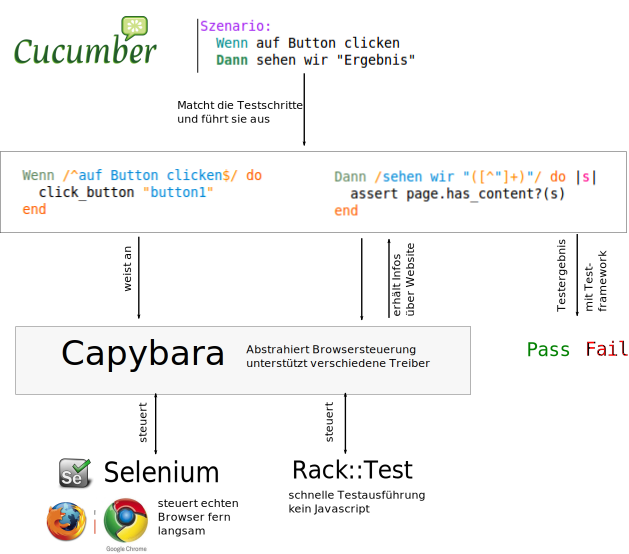
\includegraphics[width=\linewidth]{./diagrams/cucumber.pdf}
 % cucumber.pdf: 595x842 pixel, 72dpi, 20.99x29.70 cm, bb=
 \caption{Ablauf beim Akzeptanztest mit Cucumber und Capybara}
 \label{fig:cucumber}
\end{figure}

Der gesamte Ablauf eines Cucumber\index{Cucumber}-Akzeptanztests\index{Akzeptanztest} in Verbindung mit Capybara\index{Capybara} ist in Abbildung \ref{fig:cucumber} abgebildet. Cucumber matcht die definierten Testanweisungen auf die Testschritt\index{Cucumber!Testschritt}e und führt den darin enthalten Code aus. Dies kann zum Einen die Steuerung eines Webbrowsers durch Capybara sein oder zum Anderen eine Zusicherung.

\newpage\section{Code-Metriken}
Eine Codemetrik ist eine Maßzahl, die zum Vergleich dient und ein Qualitätsmerkmal für ein Stück Code oder ein Programm darstellt. Sie ist wird den Software-Metriken und Produkt-Metriken zugeordnet.

\epigraph{A function whose inputs are software data and whose output is a single
numerical value that can be interpreted as the degree to which software possesses a given attribute that affects its quality}{\cite{ieee_1998}}

Dem Verwenden von Code-Metriken liegt der Wunsch zugrunde, komplexe Codeteile auf einfache Zahlen automatisiert beurteilen zu lassen, um potenziell suboptimale Codestellen schnell zu finden, welche möglicherweise in Zukunft Defekte verursachen könnten. Aus Business-Sicht stellen Code-Metriken auch eine Methode dar, Entwicklungsfortschritt zu messen und zu beurteilen.
\subsection{Überblick über Code-Metriken und Skalen}
Hier seien nun einige der geläufigsten Code-Metriken vorgestellt.
\paragraph{Lines of Code (LOC)} ist eine häufig verwendete, und die am leichtesten zu bestimmende Größe. Sie repräsentiert den Umfang eines Programmes. Es werden alle Zeilen einer Datei gezählt, die nicht leer und keine Kommentare sind. Kommentare wiederrum können als eigene Metrik verwendet werden, um den Grad der Quelltextdokumentation zu bestimmen.

Diese Größe erhält eine größere Aussage, wenn man sie ins Verhältnis z.B. der Klasse oder eines Codefiles setzt. So kann man mit "`LOC / Klasse"' schon diejenigen Klassen finden, die wahrscheinlich zu komplex sind. \\

\paragraph{Zyklomatische Komplexität} ist ein Indikator für die Komplexität auf Basis des Kontrollflussgraphen eines Programms. Gemessen wird die Anzahl der linear unabhängigen Programmpfade. Sie ist für einen Graphen definiert durch:

\shadebox{
  $$    M = E - N + 2P $$
  \begin{center}
\begin{tabular}{ll}
   E & Anzahl der Kanten \\
   N & Anzahl der Knoten  \\
   P & Anzahl der verbundenen Komponenten \\
  \end{tabular}  \end{center}

}

In einem normalen Programm ist die Zyklomatische Komplexität die Anzahl der Entscheidungspunkte + 1 \citep[S. 314]{mccabe_complexity_1976}.

Ein daraus abgeleitetes Testverfahren "`Basis Path Testing"' schlägt vor, dass die Anzahl der Tests mindestens genauso groß sein sollte, wie die Grad der Komplexität \citep[S. 318]{mccabe_complexity_1976}. Dadurch erreicht man Branch-Coverage (C1) (Mehr zu Testabdeckung im nächsten Unterabschnitt).

\paragraph{Anzahl Bad Smells} ist eine aggregierte Metrik über Anzahl und Vorkommen von suboptimale Codestellen (\glossarpl{smell}). Diese Code-Smells sind meist ein oberflächliches Symptom für ein möglicherweise tieferliegendes Designproblem. Ob ein konkreter Smell relevant ist, muss im Einzelfall entschieden werden. Für eine grobe Übersicht genügt aber z.B. auch einfach die Summe, oder die Anzahl der Codesmells relativ zur Codemenge (Smells pro Tausend LOC). Welche Bad Smells für die Entwicklung entscheidend sind hängt von der gewählten Sprache, dem damit einhergehenden Programmierparadigma und manchmal auch den verwendeten Frameworks. Einige für Ruby relevante Smells sind z.B. (Nach \citep{kevin_rutherford_code_2010}):

\begin{description}
 \item[Geringe Kohäsion] Ist ein Oberbegriff für verschiedene andere Smells anzuwenden bei objektorientierten Programmen. Einer davon ist z.B.. "`Feature Envy"' (deutsch: Neid). Eine Klasse weiß zuviel über die internen Strukturen einer anderen Klasse, und implementiert Funktionalität, die eigentlich in jene Klasse gehören sollten. \\
 Im Beispiel würde die Berechnung eines Gesamtpreises z.B. in die Klasse \texttt{Checkout} gehören.
 \begin{lstlisting}
    @checkout.total = @checkout.total_price * MWST
 \end{lstlisting}
 \item[Nichtssagender Name] gilt für alle Programmiersprachen. Falls Bezeichner weniger als 3 Zeichen lang sind, oder Funktionen den Namen "`do"' oder "`run"' haben. Ausnahmen könnte man z.B. für die Schleifenvariable $i$ rechtfertigen
 \item[Gesetz von Demeter] bzw. die Verletzung desselben. Objekte sollten nur mit den Objekten in ihren unmittelbaren Nähe kommunizieren, und nicht etwa in Nachrichtenketten, wie z.B.:
 \begin{lstlisting}
  @job.user.address.street
 \end{lstlisting}
 Beim Law of Demeter ist eine solche Kette bis maximal Länge 1 erlaubt.
 \item[Duplikation] Offensichtliche Ähnlichkeiten zwischen Programmstücken (oder sogar Deckungsgleichheit bei Anwendung von Copy \& Paste). Fortgeschrittene Analysemethoden betrachten den Abstrakten Syntaxbaum, und können so strukturelle Ähnlichkeiten feststellen
 \end{description}

Diese Smells können mit dem Tool reek\footnote{\url{https://github.com/kevinrutherford/reek/wiki/Code-Smells}} festgestellt werden.
Weitere Informationen zu Smells und deren Beseitigung finden sie in dem Buch "`Refactoring"' von M. Fowler \citep{fowler_refactoring_1999}.

\subsection{Code-Metriken für Tests}
\label{sec:metrics}
Tests haben (auch) die Aufgabe, ein Programm oder Codestück auf Korrektheit zu untersuchen. Die Tests allerdings haben ihrerseits i.d.R. keine Tests. Um also die Nützlichkeit der eigenen Tests zu bestimmen, kann man sich aber zumindest auf Code-Metriken stützen.
Tests sind in erster Linie natürlich auch Code und können mit den oben genannten Metriken beurteilt werden. Zudem gibt es aber einige weitere exklusive Methoden, Qualität von Tests zu messen. 

\subsubsection{Verhältnis von Lines of Test zu Lines of Code}
Neben den Lines of Code kann auf dieselbe Weise die Anzahl der Codezeilen der Testklassen ermittelt werden. Daraus ermittelt sich das Verhältnis:

\shadebox{
  $$    R = \frac{\text{Lines of Code}}{\text{Lines of Test}}$$
  \begin{center}
\begin{tabular}{ll}

   $R \ll 1$ & \small Falls es deutlich weniger Testzeile (LoT), als Codezeilen (LoC) geben sollte\\
	     & \small so ist dies ein Indiz für zu wenige Tests\\
   $R > 1$   &\small Eine große Anzahl an Tests ist zwar wünschenswert, aber dies macht\\
	      & \small keine Aussage über den Vollständigkeit oder die Qualität der Tests   
  \end{tabular}  \end{center}

}

Sollte dieser deutlich kleiner als 1 sein, so ist dies ein Symptom für zu wenige Tests. Diese Zahl ist von dem Testframework und dem Programmframework stark abhängig. Gute Projekte sollten mehr Test-Code, als Programmcode besitzen, um so die Zahl der Defekte gegen 0 zu reduzieren \citep{hunt_pragmatic_1999}[S. 238]. 
        
\subsubsection{Testausführungsabdeckung}
Die Testabdeckung, misst den Grad inwieweit ein Programm getestet wurde. Die Angabe erfolgt in Prozent, wobei 100\% bedeuten, "`das Programm wurde durch die Tests komplett ausgeführt"', und 0\% "`Das Programm wurde durch die Tests überhaupt nicht berührt"' Dabei wird die vorhandene Test-Suite ausgeführt und währenddessen der entsprechende Quellcode beobachtet. Es wird festgehalten, welche Anweisungen ausgeführt wurden. Allerdings gibt es 3 Abstufungen, diese Abdeckung zu beobachten (Mit steigender Komplexität des Messverfahrens):
\begin{description}
 \item[C0] (Anweisungsüberdeckung, Statement Coverage) ist die am einfachsten zu bestimmende Abdeckung. Dabei wird geprüft, ob jede Zeile des Quellcodes während der Codeausführung mindestens einmal ausgeführt wurde
 \item[C1] (Zweigüberdeckung, Branch Coverage) prüft zusätzlich, ob jeder Zweig jeder Zeile ausgeführt wurde. Dies ist wichtig,falls man ternäre Ausdrücke\footnote{if-then-else in einer Zeile: int a = (1==1) ? 5 : 3} verwendet
 \item[C2] (Pfadüberdeckung, Path Coverage) prüft, ob jeder mögliche Codepfad durchlaufen wurde. Ein Codepfad sei eine einmalige Abfolge von Zweigen innerhalb einer Funktion von Eintritt bis Rücksprung \citep{steve_cornett_code_1996}. So werden z.B. bei 10 Bedingungen 1024 Pfade generiert, denen bei einer 100\% Abdeckung auch 1024 Tests entgegenstehen müssten.
 \end{description}
 Anmerkung: In der Literatur startet in einigen Fällen die Nummerierung bei C0 \citep{catherine_powell_abakas_2008}, in anderen Fällen aber bei C1 \citep{steve_cornett_code_1996}.
 
 Für Ruby 1.8.7 gibt es das Tool rcov \footnote{\url{http://relevance.github.com/rcov/}}, für Ruby ab 1.9.1 simple-cov\footnote{\url{https://github.com/colszowka/simplecov}}, welche beide die C0 Testabdeckung bestimmen können. Zum aktuellen Zeitpunkt sind keine weiteren Tools bekannt, um C1 oder C2 Abdeckungen zu bestimmen.
 \paragraph{Wieviel Testabdeckung ist sinnvoll oder notwendig}
 
 Beim Messen der Abdeckung stellt man sich schnell die Frage, wieviel Testabdeckung notwendig ist. Zuerst sei die Art des Messverfahrens, also C0 bis C2, wichtig. je komplexer das Messen erfolgte, desto geringer kann also die Testabdeckung am Ende ausfallen \citep{catherine_powell_abakas_2008}.
 
 Falls dem TDD-Prozess minutiös gefolgt wurde, so ist die C0 Testabdeckung immer 100\% \citep{beck_test_2002}. Für ein Rails Projekt sei es auch relativ leicht, 100\% oder nahe 100\% zu erreichen \citep{rappin_rails_2011}. Die Zahl "`100\%"' sei für sich genommen nutzlos, aber sie zu erreichen, sei für den Prozess der Testgetriebenen Entwicklung nützlich \citep[S. 270]{rappin_rails_2011}. Vielen Autoren bringen aber zum Ausdruck, dass es von der Situation abhängt \citep{infoq_2007} wieviel Testabdeckung sinnvoll ist. Test-Anfänger sollten sich zuerst überhaupt ans Testen gewöhnen, und erfahrene Entwickler sollte wissen, dass es keine einzige einfache Antwort auf diese Frage gebe \citep{infoq_2007}. Zudem gebe eine hohe Abdeckung keinen Aufschluss darüber, dass gut getestet wurde. Aber eine niedrige Zahl zeigt deutlich auf Missstände hin. Einem pragmatischen Ansatz von \citeauthor{alberto_savoia_code_2007} folgend, kann man aus dem Verhältnis der Zyklomatischen Komplexität mit der Testabdeckung eines Codestückes suboptimale Teile finden. Je mehr Verzweigung eine Methode hat, desto höher sollte ihre Testabdeckung sein \citep{alberto_savoia_code_2007}. In einem Artikel empfiehlt \citeauthor*{steve_cornett_code_1996} eine Liste von Zielen, die es je nach Budget und Zeit zu erreichen gilt, beginnend damit, dass mindestens eine Funktion in 90\% der Quelltextdateien durch die Tests aufgerufen wird bis zum finalen Schritt einer 100\% Zweiüberdeckungs-Testabdeckung \citep{steve_cornett_code_1996}.
 
 Zusammenfassend kann man sagen, dass es keine eindeutige Antwort gibt. Eine niedrige C0 Abdeckung von 50\% oder weniger zeigt allerdings deutliche Missstände beim Testverfahren an.
 
 \subsubsection{Mutations/Pertubationstests -- Defect insertion}
 \label{sec:mutation}
 Eine weitere Methode, um die Qualität von Testcode zu messen, ist der Mutationstest. Dies ist ein diversifizierendes, fehlerbasiertes Testverfahren \citep{liggesmeyer_modultest_1990}. Hierbei werden (automatisiert oder manuell) nacheinander alle Zeilen des Programmcodes geändert, und geprüft, ob danach ein Test fehlschlägt \citep{beck_test_2002}.
 
 Für Ruby gibt es ein Werkzeug, "`Heckle"`\footnote{\url{http://ruby.sadi.st/Heckle.html}}, welches dieses Verfahren implementiert. Im Detail werden Bedingungen negiert, konstante Zahlen und Funktionsaufrufe verändert, Zuweisungen verändert usw. \citep{ruby_sadists_confessions_2010}. Dabei wird immer eine Änderung (Mutation) vorgenommen, und dann alle Tests ausgeführt. Sollten dennoch in einer Mutation kein Test fehlschlagen, dass ein Test fehle, so ist die Annahme des Testverfahrens.
 
 Um hieraus eine Metrik zu gewinnen, können die Anzahl der Mutationen gemessen werden, bei denen der Test nicht fehlschlug.  
 \subsection{Notwendigkeit von Code Metriken}
 
 Code-Metriken geben dem Programmierer automatisiert und schnell ein Feedback über die Qualität seiner Arbeit. Sie helfen dabei, Probleme frühzeitig zu erkennen und die Wartbarkeit durch gezielte Refaktorisierungen nachhaltig zu verbessern. Auch psychlogische Auswirkungen dürfen nicht unterschätzt werden. Alleine der Fakt, dass Codemetriken in einem Unternehmen regelmäßig verwendet werden, motiviert den Programmierer keinen sogenannten "`Big Ball of Mud"'\footnote{Ein Antipattern, in dem ein System keinerlei offensichtliche Architektur zu haben scheint} zu schreiben. Insbesondere in kleinen Projektteams, die keine dedizierte Qualitätssicherung haben, sind Codemetriken als kostengünstiges Kontrollinstrument unerlässlich. Studien zeigen, dass der konsequente Einsatz von Code-Metriken und Analysebenchmarks die Fehlerdichte und Entwicklungskosten stark verringen kann \citep[S.10f]{baggen_standardized_2011}.
 
 Für die Testgetriebene Software dient insbesondere in der Anfangsphase die Testabdeckung als Kontrollinstrument, um zu prüfen, ob der TDD-Prozess korrekt umgesetzt wird \citep[S. 300]{nagappan_realizing_2008}. Außerdem sollte der zeitliche Verlauf der Metriken beobachtet werden, um Trends abzuschätzen und frühzeitig gegensteuern zu können. Für in \glossar{TDD} erfahrene Programmierer mag die Beobachtung der Testabdeckung nicht notwendig sein, für Einsteiger allerdings eine effektive Kontrollmöglichkeit.
 
 Nach Erfahrungen in der pludoni GmbH sind Code-Metriken ein wichtiges Feedbackinstrument, und unterstützen damit das Schreiben sauberen Codes. Wichtig ist, dass die Metriken regelmäßig berechnet werden, entweder als Cronjob oder nach jedem Einchecken in den Hauptentwicklungszweig der Versionsverwaltung, und in regelmäßigen Abständen von den Programmierern und Team-Leiter gelesen und besprochen werden. Allerdings besteht bei einer zu hohen Beobachtung der Metriken die Gefahr, eines Hawthorne-Effektes, d.h. dass die unter Beobachtung stehenden Programmierer ihr Verhalten den Code-Metriken anpassen, um optimale Ergebnisse zu erhalten \citep[52. Karte]{langr_agile_2011}, und so nur eine scheinbare Verbesserung erzielen würden.

\newpage\section{Auswahl der Entwicklungsstrategie und -Werkzeuge}
\subsection{Herausbildung einer Enticklungsstrategie für die Bedürfnisse der pludoni GmbH}
Viele der gängigen Entwicklungsstrategien, wie V-Modell oder Rational Unified Process, finden ihre Anwendung in großen Projektteams. Für mittelgroße Projektteams gibt es seit ca. 10 Jahren die agilen Prozesse. Sie haben einen eher pragmatischen Ansatz, mit dem Ziel gemeinsam mit dem Kunden eine funktionierende Software zu bauen. Zu eigen machen sie sich dabei kurze Releasezyklen, welche regelmäßig Feedback geben. Damit wird der klassische GAU am Ende des Projektes, wenn die Wünsche des Kunden mit den tatsächlichen Umsetzungen doch nicht einher gehen, vermieden. Aber viele dieser Methoden, wie z.B. SCRUM, benötigen eine Schulung für das gesamte Team, die nicht immer finanzierbar ist. 
Für die Arbeit von sehr kleinen Teams mit weniger als 4 Mitgliedern, wird nun eine Entwicklungsstrategie auf Basis der Testgetriebenen Entwicklung mit Ruby on Rails vorgestellt, die auf die Bedürfnisse der pludoni GmbH zugeschnitten ist.

Diese Bedürfnisse umfassen 
\begin{itemize}
 \item kurze Feedbackzyklen von 1 Woche
 \item Arbeit meist aus der Ferne ohne direkte Kommunikation mit den anderen Teammitgliedern. Daraus folgt ein äußerst selbstständiger Arbeitsstil
 \item möglichst fehlerfreie Software
 \item Kontinuierliche Integration
 \item pragmatisches Testen, 100\% Testabdeckung ist nicht erforderlich. Wichtige Systemlogiken, wie Bezahlvorgang und Suche müssen dagegen getestet werden. Offensichtliche CRUD\footnote{Create Read Update Delete - Die 4 Standardmethoden, die auf Ressourcen ausgeführt werden können}-Methoden müssen nicht getestet werden
 
\end{itemize}

\subsubsection{Einteilung der Features in Kategorien}
Grundsätzlich teilt die pludoni GmbH Features in zwei Kategorien ein:

\begin{enumerate}[A.]
 
 \item Features, welche in der Ansicht für Kunden und Besucher der Website sichtbar sind $\to$ Detailansichten, Listen, Bezahlvorgänge, ...
 \item Features, welche nur dem Admin sichtbar sind, oder welche im Backend ausgeführt werden $\to$ Reporting, Statistiken, Indizierung der Datenbank, Cron-Scripte, Caching, ...
\end{enumerate}

Features der \textbf{Kategorie A} sollen in Zukunft Akzeptanztestgetrieben entwickelt werden. Die Entwicklung verläuft nach dem Schema, dass in Abschnitt \ref{sec:attd} vorgestellt wurde. Die Akzeptanztests sollen in Cucumber geschrieben werden. Die Websiteinteraktion soll mithilfe von Rack:Test im Falle einer Rails-Anwendung, und mit Capybara andernfalls simuliert werden.
Ziel ist es, das bei Webanwendungen übliche wiederholte manuelle Ausprobieren mit dem Browser, auf ein Minimum zu reduzieren. Jeglicher Vorgang, den der Kunde am Browser testet, lässt sich auch als ein Akzeptanztest formulieren. Ein automatisierter Test hat zudem den Vorteil zu einem späteren Zeitpunkt leicht wiederholt zu werden. 

Der Vorteil dieser Outside-In Entwicklung ist, dass er auf den Kunden ausgerichtet ist. Die Verwendung der domänspezifischen Sprache Cucumber fördert zudem die Implementierung von Business-relevanten Features gemeinsam mit dem Kunden. Das gesamte Vokabular orientiert sich an der Anforderungsanalyse und an Businessprozessen, die auch der möglicherweise nicht-technische Kunde verstehen kann.

Für die von außen nicht-sichtbaren Features der \textbf{Kategorie B} sollen aus Kostengründen normale Unittests entwickelt nach der klassischen Testgetriebenen Entwicklung genügen. Die zusätzliche Abstraktionsebene der Akzeptanztests ist nicht notwendig.

\subsubsection{Weitere Bestandteile der Entwicklungsstrategie}

Der oben genannte Teil bezieht sich in erster Linie auf den Kunden. Weitere Praktiken, die für den Programmieralltag wichtig sind, umfassen:

\paragraph{Kontinuierliche Integration} Das Vorhandensein einer großen Test-Suite ermöglicht es, diese beim Einchecken in den Hauptzweig komplett auszuführen. Damit läßt sich sicherstellen, dass auf dem Hauptzweig eine immer lauffähige Version vorhanden ist. Die Verwendung einer Versionsverwaltung, z.B. git, ist obligatorisch.

In großen Projekten ist es üblich, komplexe Testpläne zu erstellen. Anscheinend sind aber automatisierte Tests, die bei jeden Einchecken durchgeführt werden, effektiver als rein formale Testpläne \citep{hunt_pragmatic_1999}[S. 238].

\paragraph{Code-Metriken} Ein tägliches Messen des Code-Zustandes mittels Code-Metriken ermöglicht es den Programmierern, sich selbst und gegenseitig auf die Finger zu schauen. Sollte ein Programmierer nämlich äußerst schlechten Code abgeliefert haben, so macht die Code-Analyse dies sichtbar. Dies dient in erster Linie nicht, um den Programmierer zu maßregeln, sondern ihm dabei zu helfen, den TDD-Prozess zu lernen und seinen Programmierstil ständig zu verbessern. Die Erfahrungen zeigen, dass die Programmierer meist selbst unzufrieden mit schlechtem Code, den sie geschrieben haben, sind. Code-Metriken können dabei helfen, dem Programmierer schnell ein Feedback zu seinem Code zu geben, wie es ein Code-Audit durch Andere in der Geschwindigkeit und Effizienz nie könnte.

\paragraph{Regelmäßige Paar-Programmierung} Die in Abschnitt \ref{sec:arbeitsablauf} angesprochene Dezentralisierung der Zusammenarbeit erschwert eine regelmäßige Paarprogrammierung (Pair-Programming [PP]). Nichtsdestotrotz sollten in regelmäßigen Abständen Features zu zweit entwickelt werden.  Insbesondere beim Lösen schwieriger Aufgaben und beim Anlernen neuer Teammitglieder ist Pair-Programming eine effektive Methode \citep{hulkko_multiple_2005}[S. 9]. Erfahrungsgemäß führt Pair-Programming zu besser dokumentierten Code, kann die Anzahl der Fehler verringern und zu einer höheren Arbeits-Effektivität führen \citep{hulkko_multiple_2005}.


\subsection{Auswahl der Entwicklungswerkzeuge}

Für die zukünftige Entwicklung vorrangig von Webanwendungen, werden folgende Werkzeuge berücksichtigt.

\paragraph{Werkzeuge für Tests} Die formale Beschreibungssprache \textbf{Cucumber} dient als Schnittstelle für die vom Programmierer entwickelten Testschritte. Diese könnten in einem von vielen Testframeworks geschrieben werden. Die Entscheidung viel hierbei auf Minitest (Test::Unit in Ruby 1.9), da die Syntax und Prädikate denen von JUnit und NUnit sehr ähneln, und so den Übergang zu Ruby leichter machen. Da es auch das Standard-Testframework von Ruby on Rails ist, ist so eine gute Unterstützung durch gängige Werkzeuge garantiert.

Für die Simulation eines Browsers gibt es ebenfalls verschiedene Ansätze. Als Basis fungiert dabei \textbf{Capybara}, welches unterschiedliche Browsersimulationen abstrahiert. Damit lassen sich z.B. \textbf{Selenium} ansteuern, welches wiederrum Mozilla Firefox, Internet Explorer oder Google Chrome fernsteuern kann. Dies ist allerdings sehr langsam, da ein kompletter Browser gestartet und ferngesteuert wird. Daher ist die Nutzung von Selenium nur für das Testen von möglicherweise problematischen Interaktionen und das Testen von Javascript notwendig. Für alle anderen Fälle kann man auf RackTest zurückgreifen, welches extrem schnell eine Rack-Anwendung\footnote{Rack ist ein minimales Interface zwischen Webserver und Webanwendung -- Ruby on Rails ist eine solche Rack Anwendung} simuliert.
Falls in Zukunft mehr Geschwindigkeit in der Testausführung, insbesondere bei den Selenium-Tests, gewünscht wird, so kann man auf Parallelisierung auf mehreren Computern zurückgreifen.

Für ein unmittelbares Feedback sind auch automatische Test-Runner erwünscht. Hierbei gibt es z.B. \textbf{autotest} und \textbf{guard}. Diese Programme beobachten den Projektbaum, und führen bei Änderung der Dateien automatisch die relevanten Tests aus. Um die Geschwindigkeit, und damit den Feedbackzyklus zu verbessern, können diese Programme so gesteuert werden, dass sie nur den Testfall ausführen, an dem gerade gearbeitet wird. 

Durch \textbf{spork} lässt sich eine RoR-Anwendung starten und im Hintergrund halten, so dass eine erneute Testausführung deutlich schneller von statten geht, als wenn die komplette Anwendung neu geladen werden müsste.

    
\paragraph{Werkzeuge für Code-Metriken}  Für die Generierung von Code-Metriken dient das Ruby-Gem "`metric-fu"', welches seinerseits über verschiedene Code-Metriken Zusammenfassungen bildet und diese auch zeitlich darstellen kann. Darunter fallen z.B. die Zyklomatische Komplexität, den Grad der Duplikationen, verschiedene Code-Smells, Nutzung der Versionsverwaltung und Testabdeckung.

Die Testabdeckung wird durch simple-cov berechnet, welches eine C0 Code Coverage bestimmt.

\paragraph{Texteditoren} Innerhalb der Entwickler der pludoni GmbH besteht ein Konsens für die Verwendung von vim, da hier bereits eine große Basis an Plugins gesammelt wurde, die die Entwicklung von Webanwendungen und insbesondere Ruby on Rails erleichtern. Ein weiterer Vorteil ist es, dass vim ohne ein graphisches Interface auskommt, und so direkt von der Shell auf dem Webserver ausgeführt werden kann.
Nichtsdestotrotz sei es zukünftigen Entwicklern freigestellt, eine IDE, wie Eclipse mit dem Plugin RadRails oder Netbeans zu verwenden.

\subsection{Diskussion der Maßnahmen}
TODO Zusammenfassung evtl ins Fazit oder Auswertung

Viele dieser Maßnahmen dienen dazu, den Feedbackzyklus so kurz wie möglich zu halten. Für eine Testgetriebene Entwicklung ist es unerlässlich, dass die Testausführung schnell abläuft. Andernfalls, so die Erfahrung, führt dies zu einer verminderten Ausführungsrate, und ist damit hinderlich für die Entwicklung von sauberen Code.

Durch die gewählte Entwicklungsstrategie kann sogar die Anforderungsanalyse und Abnahme testgetrieben durchgeführt werden. 
\newpage\chapter{Anwendung der Testgetriebenen Entwicklung}
\label{sec:awtdd}

In den nachfolgenden Abschnitten wird examplarisch an dem Objekt "`Job"', also der internen Repräsentation einer Stellenanzeige, die Testgetriebene\index{TDD} Entwicklung mit praktischen Beispielen näher erläutert.
Besonderes Augenmerk soll dabei auf den Entwicklungsfluss von \glossar{TDD}\index{TDD} gelegt werden. Zu dessen Verdeutlichung ist am Dokumentenrand die jeweilige Phase innerhalb des TDD-Zyklus zu finden (Red, Green, Refactor), der die im Text gezeigten Codeabschnitte zuzuordnen sind.

Ziel dieses Kapitels wird es sein, einen Überblick über die Art und Weise zu erhalten, mit der die verschiedenen Teilbereiche einer Webanwendung testgetrieben entwickelt werden können.
Die ersten beiden Abschnitte richten sich an zwei der Grundbausteine einer \glossar{MVC} (vgl. Abschnitt \ref{sec:railsconcepts})-Webanwendung, die Modell\index{Ruby-on-Rails!Modell}- und Controller\index{Ruby-on-Rails!Controller}tests. Im dritten Abschnitt sehen wir, wie Test Doubles verwendet werden können, um Zugriffe auf externe Datenlieferanten zu simulieren. Danach betrachten wir die Anwendung aus Anwendersicht und widmen wir uns der Implementierung von Akzeptanz\index{Akzeptanztest}- und Systemtests (vgl. Abschnitt \ref{sec:acceptance}).
Zum Schluss gibt es einen Ausblick auf das Testen von JavaScript\index{JavaScript}-Ereignissen.

\section{Implementierung von Unit-Tests (Modelltests)}    
\label{sec:awunit}

Ein Rails-Modell, wie in \ref{sec:railsconcepts} auf S. \pageref{sec:railsconcepts} beschrieben, repräsentiert die Daten der Anwendung, und die Regeln, wie diese zu verändern sind. Bei Rails werden sie hauptsächlich dazu verwendet, um mit der zugrundeliegenden Datenbanktabelle zu interagieren. Per Konvention von Rails findet hier die Hauptarbeit, also die Business-Logik, statt.

Fast jeder Unittest bei Rails beinhaltet das Testen auf Validierungskritieren seines korrespondierenden Modells, d.h. wann eine Instanz dieses Modells gültig ist und damit gespeichert werden darf (man denke z.B. an Pflichtfelder für ein Modell "`Nutzer"` oder die Validierung des Formates seiner E-Mail-Adresse). Weiterhin sollten natürlich alle weiteren, selbstdefinierten, Methoden getestet werden.

Diese Validierungen werden durch das \glossar{ORM}-Framework ActiveRecord, welches Rails standardmäßig nutzt, bereitgestellt. Bevor wir weiter auf die 

\paragraph{1. Der Anfang}
\begin{figure}[htbp]
 \centering

 \includegraphics[width=0.3\textwidth]{./diagrams/job-erm.png}
 % job-erm.png: 173x186 pixel, 51dpi, 8.65x9.30 cm, bb=0 0 245 264
 \caption{Attribute des Modells "`Job"'}
  \label{fig:job-erm}
\end{figure}

Während der Analyse wurden die benötigten Attribute bestimmt. In Abbildung \ref{fig:job-erm} sei z.B. ein Fragment des Grobdesigns, in dem die Basisattribute der Tabelle dargestellt werden. Neben den einfachen Attributen, wie Title, Description und Link, existieren auch Referenzen auf andere Objekte (d.h. dies stellen Fremdschlüssel zu anderen Tabellen dar), wie z.B. Schlagwörter (Tags), ein Besitzer einer Stellenanzeige (User) und so weiter.

Einer der häufigsten Wege, ein Modell und dessen Datenbankschema zu generieren, ist die Nutzung des mitgelieferten Codegenerators. Mittels des Kommandos:

\shadebox{  
  rails generate model \textit{MODELLNAME} spalte1:datentyp1 spalte2:datentyp2 ...
}

generieren wird ein Modell mit dem angegebenen Modellnamen. Dazu geben wir paarweise die gewünschten Spaltennamen und deren Datentypen an (\texttt{string, text, datetime, references, integer, boolean, decimal}, ...).
\begin{lstlisting}
~/it-jobs$ rails generate model job title:string link:string \
    description:text user:references visible:boolean

      invoke  active_record
      create    db/migrate/20110828160636_create_jobs.rb
      create    app/models/job.rb
      invoke    test_unit
      create      test/unit/job_test.rb
      create      test/fixtures/jobs.yml

\end{lstlisting}
Mit der Anweisung uns ein Modell \texttt{job} mit den nachfolgenden Attributen zu generieren, hat Rails uns nun schon ein Stück Arbeit abgenommen. Dabei delegiert der Codegenerator \texttt{model} nun die Arbeit an den Codegenerator für ein ActiveRecord-Model (erkennbar an dem \texttt{invoke active\_record}). Dieser wiederrum generiert 2 Dateien und ruft seinerseits einen Codegenerator zum Generieren der Tests auf (\texttt{invoke test\_unit})

Es wurden erstellt:
\begin{itemize}
 \item Eine Migration (\verb|db/migrate/2011xxxxxx_create_jobs.rb|). Dies stellt eine datenbankunabhängige Repräsentation einer Änderung an der Struktur unserer Datenbank dar. In diesem ist es die Erstellung einer Tabelle \texttt{jobs} (beachte: Plural!), mit den Spalten Titel, Link als String, Description als Textfeld, eine User\_ID als Referenz auf ein anderes Modell usw.
 \item Die Modelklasse (\verb|app/models/job.rb|). Trotz unserer Definition der Spalten und deren Typen über die Kommandozeile, ist diese Klasse leer. Da wir ActiveRecord verwenden, definieren wir die Attribute, die unser Modell hat, nicht in der Modellklasse, sondern ausschließ in der Datenbank. Die Migration erspart uns die manuelle Arbeit, selbst in unserer Datenbank Spalten anzulegen. Bei Initialisierung eines Modells lädt ActiveRecord die Spalteninformationen aus der Datenbank, und generiert dafür Getter und Setter Methoden. 
 \item Die dazugehörige Testklasse (\verb|app/unit/job_test.rb|)
 \item und Fixtures-Datei (\verb|test/fixtures/jobs.yml|), zur Definition von Testdaten. 
\end{itemize}

Die Migration liegt nun zwar vor, aber es existiert noch keine Datenbank und demnach auch noch keine Tabelle mit dem Namen \texttt{jobs}. 
Wir wollen Rails nun mitteilen, dass es die Migration anwenden soll, um damit die Datenbank und Tabelle zu erstellen

Rails stellt uns mittels des Kommandozeilenwerkzeugs \textbf{rake} eine Schnittstelle zu unserer Anwendung bereit, mit der wir meist Wartungsaufgabe ausführen können. Rake erwartet die Angabe eines Tasks, und optional die Angabe einer Umgebungsvariable für die Rails-Umgebung, in der der Test ausgeführt werden soll\footnote{Jede Umgebung verfügt normalerweise über eine eigene Datenbank. standardmäßig befinden wir uns in der "`Development"'-Umgebung}.

\shadebox{  \centering
  rake \textit{TASK} [RAILS\_ENV=production]
}

Dazu weisen wir nun Rails an, alle offenen Migrationen auszuführen. Standardmäßig erstellt Rails dann selbstständig eine SQLite Datenbank unter \texttt{db/development.sqlite3}.


\begin{lstlisting}
$ rake db:migrate 
 
==  CreateJobs: migrating =========================
-- create_table(:jobs)
   -> 0.0020s
==  CreateJobs: migrated (0.0021s) ================
\end{lstlisting}

Danach können wir die Rails-Test-Suite mithile eines weitere Rake-Tasks auch schon ausführen. Dieser Rake-Task legt selbsständig eine Testdatenbank an, führt offene Migrationen darauf aus und führt dann alle vorhanden Tests aus.

\begin{lstlisting}
$ rake test
(in /home/zealot64/TEST)
Loaded suite /usr/lib/ruby/gems/1.8/gems/rake-0.8.7/lib/rake/rake_test_loader
Started
.
Finished in 0.043818 seconds.

1 tests, 1 assertions, 0 failures, 0 errors
\end{lstlisting}

Es wurde also schon ein Testfall erfolgreich ausgeführt, nämlich ein Dummytestfall von Rails:

\begin{ruby}[label={test/units/job\_test.rb}]
\PY{c+c1}{#test/unit/job\PYZus{}test.rb }
\PY{n+nb}{require} \PY{l+s+s1}{'test\PYZus{}helper'}

\PY{k}{class} \PY{n+nc}{JobTest} \PY{o}{<} \PY{n+no}{ActiveSupport}\PY{o}{::}\PY{n+no}{TestCase}
  \PY{c+c1}{# Replace this with your real tests.}
  \PY{n+nb}{test} \PY{l+s+s2}{"}\PY{l+s+s2}{the truth}\PY{l+s+s2}{"} \PY{k}{do}
    \PY{n}{assert} \PY{k+kp}{true}
  \PY{k}{end}
\PY{k}{end}
\end{ruby}
\label{list:bla}
\codecaption{Standardtest generiert durch Rails}


\paragraph{2. Testen auf Validierung}

Ein Feature von Rails umfassen die sogenannten Validierungen. Diese stellen sicher, dass eine Instanz eines Modells nur dann gespeichert ist, wenn es gewissen Kritieren entspricht. Viele der Validations sind vergleichbar mit den Datenbank-Constraints einiger Datenbanken. Rails nutzt diese standardmäßig nicht, da es auch andere Persistenzsysteme unterstützt, wie z.B. Key-Value-Store oder sogenannte NoSQL Datenbanken. So stellt Rails die Konsistenz und referenzielle Integrität innerhalb der Applikationsschicht sicher.

Nun möchten wir sicherstellen, dass eine Stellenanzeige nur dann gespeichert wird, wenn sie einen Titel beinhaltet. Der Test dazu würde wie folgt lauten:

\begin{ruby}[label={test/units/job\_test.rb}]
\PY{n+nb}{require} \PY{l+s+s1}{'test\PYZus{}helper'}

\PY{k}{class} \PY{n+nc}{JobTest} \PY{o}{<} \PY{n+no}{ActiveSupport}\PY{o}{::}\PY{n+no}{TestCase}
  \PY{n+nb}{test} \PY{l+s+s2}{"}\PY{l+s+s2}{ein Job muss einen Titel haben}\PY{l+s+s2}{"} \PY{k}{do}
    \PY{n}{job} \PY{o}{=} \PY{n+no}{Job}\PY{o}{.}\PY{n}{new}
    \PY{n}{job}\PY{o}{.}\PY{n}{title} \PY{o}{=} \PY{k+kp}{nil}
    \PY{n}{assert} \PY{o}{!}\PY{n}{job}\PY{o}{.}\PY{n}{save}
  \PY{k}{end}
\PY{k}{end}
\end{ruby}
\codecaption{Test auf Vorhandensein eines Titels}
\tddred
Zuerst instanziieren wir einen Job, und geben ihm explizit einen leeren Titel, um das Testziel nochmal herauszustellen. Danach rufen wir die \texttt{save}-Methode auf, die prüft, ob alle Validierungskritierien erfolgt sind, und speichert das Objekt persistent in der Datenbank im Erfolgsfall. Dann gibt \texttt{save} ein \texttt{true} zurück, anderfalls, d.h. wenn die Validierung fehlschlug, \texttt{false}.
Der Ablauf ist in der Abbildung \ref{fig:activerecordsave} noch einmal erläutert.

\begin{figure}[hbp]
 \centering
 \includegraphics[width=0.8\textwidth]{./diagrams/activerecord-save.pdf}
 % activerecord-save.pdf: 595x675 pixel, 72dpi, 20.99x23.81 cm, bb=0 0 595 675
 \caption{Funktionsweise von save bei ActiveRecord Objekten}
 \label{fig:activerecordsave}
\end{figure}

Da wir noch keine Validierungskritieren implementiert haben, schlägt dieser Test fehl, da das Objekt gespeichert wurde.

Unser nächstes Ziel ist es nun, mit so wenig Code wie möglich den Test bestehen zu lassen. Das können wir mittels der eingebauten wie schon erwähnten Validierungen:

\begin{ruby}[label=app/models/job.rb]
\PY{k}{class} \PY{n+nc}{Job} \PY{o}{<} \PY{n+no}{ActiveRecord}\PY{o}{::}\PY{n+no}{Base}
  \PY{n}{validates} \PY{l+s+ss}{:title}\PY{p}{,} \PY{l+s+ss}{:presence} \PY{o}{=}\PY{o}{>} \PY{k+kp}{true}
\PY{k}{end}
\end{ruby}
\codecaption{Implementierung der Validierung in die Klasse Job}
\texttt{validates} ist eine Funktion aus der ActiveRecord Bibliothek, die zwei Parameter entgegennimmt: Der erste ist die Spalte, auf der sich die Validierung bezieht, als Zweites folgt eine Liste an Validierungskritieren. Hier ist das Kritierum \texttt{presence}, also das Vorhandensein eines nicht-leeren Attributs. Weitere Kritieren sind z.B. Format, Länge, Minimum, Maximum, oder selbst definierte Kriterien.

\tddgreen
Nach erneuter Ausführung der Testsuite, besteht der Test nun. Jetzt folgt die Refaktorisierungsphase. Der Programmcode lässt sich nicht weiter vereinfachen. Aber der Testcode ist ausdrücklich nicht von Refaktorisierungen befreit, und eine Refaktorisierung wäre z.B.:
\tddrefactor
\begin{ruby}[label=test/unit/job\_test.rb]
\PY{n+nb}{test} \PY{l+s+s2}{"}\PY{l+s+s2}{ein Job muss einen Titel haben}\PY{l+s+s2}{"} \PY{k}{do}
  \PY{n}{job} \PY{o}{=} \PY{n+no}{Job}\PY{o}{.}\PY{n}{new} \PY{l+s+ss}{:title} \PY{o}{=}\PY{o}{>} \PY{k+kp}{nil}
  \PY{n}{assert} \PY{o}{!}\PY{n}{job}\PY{o}{.}\PY{n}{save}
\PY{k}{end}
\end{ruby}
\codecaption{refaktorisierter Test}

Nun wollen wir dasselbe für das Feld E-Mail tun, hierbei aber nicht nur das Vorhandensein prüfen, sondern auch das Format.

\begin{ruby}[label=test/unit/job\_test.rb]
\PY{n+nb}{test} \PY{l+s+s2}{"}\PY{l+s+s2}{ein Job muss eine gültige E-Mail haben}\PY{l+s+s2}{"} \PY{k}{do}
  \PY{n}{job} \PY{o}{=} \PY{n+no}{Job}\PY{o}{.}\PY{n}{new} \PY{l+s+ss}{:email} \PY{o}{=}\PY{o}{>} \PY{l+s+s2}{"}\PY{l+s+s2}{invalid\PYZus{}email}\PY{l+s+s2}{"}
  \PY{n}{assert} \PY{o}{!}\PY{n}{job}\PY{o}{.}\PY{n}{save}
\PY{k}{end}
\end{ruby}
\tddred
Die Implementierung wäre dann:
\begin{ruby}[label=app/models/job.rb]
\PY{k}{class} \PY{n+nc}{Job} \PY{o}{<} \PY{n+no}{ActiveRecord}\PY{o}{::}\PY{n+no}{Base}
  \PY{n}{validates} \PY{l+s+ss}{:email}\PY{p}{,} \PY{l+s+ss}{:format} \PY{o}{=}\PY{o}{>} \PY{l+s+sr}{/}\PY{l+s+sr}{\PYZca{}[}\PY{l+s+sr}{\PYZbs{}}\PY{l+s+sr}{w}\PY{l+s+sr}{\PYZbs{}}\PY{l+s+sr}{d\PYZus{}}\PY{l+s+sr}{\PYZbs{}}\PY{l+s+sr}{-]+@[}\PY{l+s+sr}{\PYZbs{}}\PY{l+s+sr}{w}\PY{l+s+sr}{\PYZbs{}}\PY{l+s+sr}{d\PYZus{}}\PY{l+s+sr}{\PYZbs{}}\PY{l+s+sr}{-]}\PY{l+s+sr}{\PYZbs{}}\PY{l+s+sr}{.[}\PY{l+s+sr}{\PYZbs{}}\PY{l+s+sr}{w}\PY{l+s+sr}{\PYZbs{}}\PY{l+s+sr}{d]\PYZob{}2,3\PYZcb{}\$}\PY{l+s+sr}{/}
  \PY{o}{.}\PY{n}{.}\PY{o}{.}
\PY{k}{end}
\end{ruby}
\tddgreen
Eine Refaktorisierung ist aufgrund der Einfachheit der Beispiel hier nur gering möglich. Man könnte z.B. den regulären Ausdruck, der das Format der E-Mail Adresse beschreibt in eine neue Klasse oder zumindest eine Konstante auslagern. Wir wählen eine Konstante, die beim Laden von Rails bereitgestellt wird.
\tddrefactor
\begin{ruby}[label=config/initializers/job.rb und app/models/job.rb]
\PY{c+c1}{# config/initializers/regex.rb}
\PY{n+no}{REGEX\PYZus{}EMAIL\PYZus{}FORMAT} \PY{o}{=} \PY{l+s+sr}{/}\PY{l+s+sr}{\PYZca{}[}\PY{l+s+sr}{\PYZbs{}}\PY{l+s+sr}{w}\PY{l+s+sr}{\PYZbs{}}\PY{l+s+sr}{d\PYZus{}}\PY{l+s+sr}{\PYZbs{}}\PY{l+s+sr}{-]+@[}\PY{l+s+sr}{\PYZbs{}}\PY{l+s+sr}{w}\PY{l+s+sr}{\PYZbs{}}\PY{l+s+sr}{d\PYZus{}}\PY{l+s+sr}{\PYZbs{}}\PY{l+s+sr}{-]}\PY{l+s+sr}{\PYZbs{}}\PY{l+s+sr}{.[}\PY{l+s+sr}{\PYZbs{}}\PY{l+s+sr}{w}\PY{l+s+sr}{\PYZbs{}}\PY{l+s+sr}{d]\PYZob{}2,3\PYZcb{}\$}\PY{l+s+sr}{/}

\PY{c+c1}{# app/models/job.rb}
\PY{k}{class} \PY{n+nc}{Job} \PY{o}{<} \PY{n+no}{ActiveRecord}\PY{o}{::}\PY{n+no}{Base}
  \PY{n}{validates} \PY{l+s+ss}{:email}\PY{p}{,} \PY{l+s+ss}{:format} \PY{o}{=}\PY{o}{>} \PY{n+no}{REGEX\PYZus{}EMAIL\PYZus{}FORMAT}
    \PY{o}{.}\PY{n}{.}\PY{o}{.}
\PY{k}{end}
\end{ruby}
\codecaption{Auslagerung des Regulären Ausdrucks in einen Initalisierer}
Ein erneutes Ausführen der Tests betätigt den Erfolg der Refaktorisierung.

\paragraph{3. Refaktorisierungen der Testklasse}
Nun fehlt aber noch die Definition eines Positiv-Beispiel für einen gültigen Job.

\begin{ruby}[label=test/unit/job\_test.rb]
...
\PY{n+nb}{test} \PY{l+s+s2}{"}\PY{l+s+s2}{ein vollstaendiger Job muss gueltig seinn}\PY{l+s+s2}{"} \PY{k}{do}
  \PY{n}{job} \PY{o}{=} \PY{n+no}{Job}\PY{o}{.}\PY{n}{new} \PY{l+s+ss}{:title} \PY{o}{=}\PY{o}{>} \PY{l+s+s2}{"}\PY{l+s+s2}{Rails Entwickler}\PY{l+s+s2}{"}\PY{p}{,} \PY{l+s+ss}{:email} \PY{o}{=}\PY{o}{>} \PY{l+s+s2}{"}\PY{l+s+s2}{info@stefanwienert.net}\PY{l+s+s2}{"}
  \PY{n}{assert\PYZus{}valid} \PY{n}{job}
\PY{k}{end}
\end{ruby}
\tddgreen
Dieser Test besteht sofort, macht also genau genommen keine weitere Aussage über unser System. Nach der "`reinen"' Testgetriebenen Leere sollte dieser entfernt werden. Es ist allerdings eine gute Strategie, bei Validierungen mindestens ein Beispiel zu präsentieren, dass angenommen wird. Nichtsdestotrotz können wir nun Refaktorisieren. Insbesondere unsere Testfunktionen enthalten unnötige Redundanzien:

\begin{ruby}[label=test/unit/job\_test.rb]
\PY{n+nb}{test} \PY{l+s+s2}{"}\PY{l+s+s2}{ein Job muss einen Titel haben}\PY{l+s+s2}{"} \PY{k}{do}
  \PY{n}{job} \PY{o}{=} \PY{n+no}{Job}\PY{o}{.}\PY{n}{new} \PY{l+s+ss}{:title} \PY{o}{=}\PY{o}{>} \PY{k+kp}{nil}
  \PY{n}{assert} \PY{o}{!}\PY{n}{job}\PY{o}{.}\PY{n}{save}
\PY{k}{end}
\PY{n+nb}{test} \PY{l+s+s2}{"}\PY{l+s+s2}{ein Job muss eine gültige E-Mail haben}\PY{l+s+s2}{"} \PY{k}{do}
  \PY{n}{job} \PY{o}{=} \PY{n+no}{Job}\PY{o}{.}\PY{n}{new} \PY{l+s+ss}{:email} \PY{o}{=}\PY{o}{>} \PY{l+s+s2}{"}\PY{l+s+s2}{invalid\PYZus{}email}\PY{l+s+s2}{"}
  \PY{n}{assert} \PY{o}{!}\PY{n}{job}\PY{o}{.}\PY{n}{save}
\PY{k}{end}
\PY{n+nb}{test} \PY{l+s+s2}{"}\PY{l+s+s2}{ein vollstaendiger Job muss gueltig seinn}\PY{l+s+s2}{"} \PY{k}{do}
  \PY{n}{job} \PY{o}{=} \PY{n+no}{Job}\PY{o}{.}\PY{n}{new} \PY{l+s+ss}{:title} \PY{o}{=}\PY{o}{>} \PY{l+s+s2}{"}\PY{l+s+s2}{Rails Entwickler}\PY{l+s+s2}{"}\PY{p}{,} \PY{l+s+ss}{:email} \PY{o}{=}\PY{o}{>} \PY{l+s+s2}{"}\PY{l+s+s2}{info@stefanwienert.net}\PY{l+s+s2}{"}
  \PY{n}{assert\PYZus{}valid} \PY{n}{job}
\PY{k}{end}
\end{ruby}
\codecaption{Alle bisherigen Testmethoden in der Klasse JobTest}
\tddrefactor
In allen drei Methoden wird ein Job instanziiert, und lediglich verschiedene Attribute überprüft. Auch haben unsere ersten beiden Tests keine gültige Aussage mehr, da der jeweilige Job sowieso nicht gültig ist, da jeweils das andere Attribut fehlt\footnote{Im ersten Test ist nicht nur der Titel nicht gesetzt, sondern auch die E-Mail entspricht nicht dem Format}. Es ist also höchste Zeit, die Tests zu refaktorisieren. Dies geschieht am Besten durch die Verwendung einer Testdaten-Generation, z.B. den eingebauten Fixtures, die Rails uns bei der Codegeneration schon mit generiert hatte. Dabei definieren wir zentralisiert unsere (gültigen) Testdaten, die von Rails vor jedem einzelnen Test in der Datenbank bereitgestellt werden:

\begin{ruby}[label=test/fixtures/jobs.yml]
\PY{l+lScalar+lScalarPlain}{valid\PYZus{}job}\PY{p+pIndicator}{:}
  \PY{l+lScalar+lScalarPlain}{title}\PY{p+pIndicator}{:} \PY{l+lScalar+lScalarPlain}{Rails}\PY{l+lScalar+lScalarPlain}{ }\PY{l+lScalar+lScalarPlain}{Entwickler}
  \PY{l+lScalar+lScalarPlain}{email}\PY{p+pIndicator}{:} \PY{l+lScalar+lScalarPlain}{info@stefanwienert.net}
  \PY{l+lScalar+lScalarPlain}{link}\PY{p+pIndicator}{:} \PY{l+s}{"}\PY{l+s}{http://www.example.com/jobs}\PY{l+s}{"}
  \PY{l+lScalar+lScalarPlain}{visible}\PY{p+pIndicator}{:} \PY{l+lScalar+lScalarPlain}{true}
  \PY{l+lScalar+lScalarPlain}{...}
\PY{l+lScalar+lScalarPlain}{invisible\PYZus{}job}\PY{p+pIndicator}{:}
  \PY{l+lScalar+lScalarPlain}{title}\PY{p+pIndicator}{:} \PY{l+lScalar+lScalarPlain}{Rails}\PY{l+lScalar+lScalarPlain}{ }\PY{l+lScalar+lScalarPlain}{Entwickler}
  \PY{l+lScalar+lScalarPlain}{visible}\PY{p+pIndicator}{:} \PY{l+lScalar+lScalarPlain}{false}
  \PY{l+lScalar+lScalarPlain}{...}
\end{ruby}
\codecaption{Fixtures Testdaten für zwei Jobs}

Nun können wir diese Fixtures in unseren Tests verwenden, und das ganze in einer \texttt{setup}-Methode, die vor jedem Testfall aufgerufen wird, laden:
\tddrefactor
\begin{ruby}[label=test/unit/job\_test.rb]
\PY{k}{class} \PY{n+nc}{JobTest} \PY{o}{<} \PY{n+no}{ActiveSupport}\PY{o}{::}\PY{n+no}{TestCase}
  \PY{n}{setup} \PY{k}{do}
    \PY{n+nv+vi}{@job} \PY{o}{=} \PY{n}{jobs} \PY{l+s+ss}{:valid\PYZus{}job}
    \PY{c+c1}{# Dies lädt den Job mit dem Schlüssel "valid\PYZus{}job" und schreibt ihn }
    \PY{c+c1}{#  in die Instanzvariable @job der Testklasse}
  \PY{k}{end}
  \PY{n+nb}{test} \PY{l+s+s2}{"}\PY{l+s+s2}{stelle sicher, dass die Fixtures valide sind}\PY{l+s+s2}{"} \PY{k}{do}
    \PY{n}{assert\PYZus{}valid} \PY{n+nv+vi}{@job}
  \PY{k}{end}
  \PY{n+nb}{test} \PY{l+s+s2}{"}\PY{l+s+s2}{ein Job muss einen Titel haben}\PY{l+s+s2}{"} \PY{k}{do}
    \PY{n+nv+vi}{@job}\PY{o}{.}\PY{n}{title} \PY{o}{=} \PY{k+kp}{nil}
    \PY{n}{assert} \PY{o}{!}\PY{n+nv+vi}{@job}\PY{o}{.}\PY{n}{save}
  \PY{k}{end}
  \PY{n+nb}{test} \PY{l+s+s2}{"}\PY{l+s+s2}{ein Job muss eine gültige E-Mail haben}\PY{l+s+s2}{"} \PY{k}{do}
    \PY{n+nv+vi}{@job}\PY{o}{.}\PY{n}{email} \PY{o}{=} \PY{l+s+s2}{"}\PY{l+s+s2}{invalid\PYZus{}email}\PY{l+s+s2}{"}
    \PY{n}{assert} \PY{o}{!}\PY{n+nv+vi}{@job}\PY{o}{.}\PY{n}{save}
  \PY{k}{end}
\PY{k}{end}
\end{ruby}
\codecaption{Finale Job-Test Klasse nach Refaktorisierung}



Am Ende dieser Refaktorisierungen ist es notwendig, die Tests noch einmal auszuführen.
\tddgreen
Danach würde die Implementierung einer nächsten Teilanforderung sein. 

In diesem Abschnitt war zu sehen, dass die Testgetriebene Entwicklung das Arbeiten und Testen in kleinen Schritten favorisiert.

\section{Implementierung von Controller-Tests (functional tests)}
\epigraph{Skinny Controller, Fat Model [...] Try to keep your controller actions and views as slim as possible.}{Jamis Buck, Programmierer bei 37signals}


Neben den Unittest\index{Test!Unittest}s stellt Ruby on Rails\index{Ruby-on-Rails} eine weitere Testart nativ bereit. Technisch gesehen handelt es sich bei diesen Functional Tests aber auch um Unittests, da deren Testobjekt eine Klasse, der Controller, ist. 
Ein Controller hat bei Ruby on Rails\index{Ruby-on-Rails} die Aufgabe, Anfragen für bestimmte Routen, also Web-Adressen, anzunehmen, die Arbeit an eine Modelklasse auszulagern, und eine View aufzurufen, die letztendlich HTML-Code generiert.

Im ersten Beispiel wollen wir testen, dass ein Gast-Nutzer, also z.B. ein Bewerber, eine sichtbare Stellenanzeige aufrufen darf (\texttt{visible = true}). Hierbei verwenden wir wieder unser oben definiertes Fixture für einen gültigen Job.
% SNIPPET: 
%                                                                                                                                                                    
% /test/functional/jobs_controller_test.rb                                                                                                                           
% require 'test_helper'                                                                                                                                              
%                                                                                                                                                                    
% class JobsControllerTest < ActionController::TestCase                                                                                                              
%   test "Gast Nutzer kann Stellen betrachten" do                                                                                                                    
%     session[:user_id] = nil                                                                                                                                        
%     job = jobs(:valid_job)                                                                                                                                         
%                                                                                                                                                                    
%     get :show, :id => job.id                                                                                                                                       
%                                                                                                                                                                    
%     assert_response :success                                                                                                                                       
%     assert_equal job, assigns(:job)                                                                                                                                
%   end                                                                                                                                                              
% end                                                                                                                                                                
\begin{ruby}[label=test/functional/jobs\_controller\_test.rb]
\PY{n+nb}{require} \PY{l+s+s1}{'test\PYZus{}helper'}

\PY{k}{class} \PY{n+nc}{JobsControllerTest} \PY{o}{<} \PY{n+no}{ActionController}\PY{o}{::}\PY{n+no}{TestCase}
  \PY{n+nb}{test} \PY{l+s+s2}{"}\PY{l+s+s2}{Gast Nutzer kann Stellen betrachten}\PY{l+s+s2}{"} \PY{k}{do}
    \PY{n}{session}\PY{o}{[}\PY{l+s+ss}{:user\PYZus{}id}\PY{o}{]} \PY{o}{=} \PY{k+kp}{nil}
    \PY{n}{job} \PY{o}{=} \PY{n}{jobs}\PY{p}{(}\PY{l+s+ss}{:valid\PYZus{}job}\PY{p}{)}
    
    \PY{n}{get} \PY{l+s+ss}{:show}\PY{p}{,} \PY{l+s+ss}{:id} \PY{o}{=}\PY{o}{>} \PY{n}{job}\PY{o}{.}\PY{n}{id}
    
    \PY{n}{assert\PYZus{}response} \PY{l+s+ss}{:success}
    \PY{n}{assert\PYZus{}equal} \PY{n}{job}\PY{p}{,} \PY{n}{assigns}\PY{p}{(}\PY{l+s+ss}{:job}\PY{p}{)}
  \PY{k}{end}
\PY{k}{end}
\end{ruby}
\codecaption{JobsController-Test: Gast Nutzer darf Stellen betrachten}

\tddred
Zuerst loggen wir jeglichen Nutzer aus, der eventuell eingeloggt war, dann laden wir das Fixture und führen einen simulierten HTTP Request auf die Detailansicht der Stellenanzeige aus (Die Aktion \texttt{show} mit der ID des Jobs).
Nun erwarten wir, dass wir einen HTTP-Status Code 200 (Erfolg) erhalten, und dass der Controller eine Variable \texttt{@jobs} bereitstellt, die mit unserem Fixture identisch ist.

Die Implementation dieser Anforderung könnte wie folgt umgesetzt werden:
% -------------------------------
% SNIPPET: 
%                                                                                                                                                                    
% # app/controllers/jobs_controller.rb                                                                                                                               
% class JobsController < ApplicationController                                                                                                                       
%   ...                                                                                                                                                              
%   def show                                                                                                                                                         
%     @job = Job.first                                                                                                                                               
%   end                                                                                                                                                              
%   ...                                                                                                                                                              
%                                                                                                                                                                    
% end                                                                                                                                                                
\begin{ruby}[label=app/controllers/jobs\_controller.rb]
\PY{k}{class} \PY{n+nc}{JobsController} \PY{o}{<} \PY{n+no}{ApplicationController}
  \PY{o}{.}\PY{n}{.}\PY{o}{.}
  \PY{k}{def} \PY{n+nf}{show}
    \PY{n+nv+vi}{@job} \PY{o}{=} \PY{n+no}{Job}\PY{o}{.}\PY{n}{first}
  \PY{k}{end}
  \PY{o}{.}\PY{n}{.}\PY{o}{.}
\PY{k}{end}
\end{ruby}
\codecaption{JobsController: Erfüllung des Tests durch eine Fake-Implementierung}

\tddgreen
Das Laden des erstem Jobs aus unserer Datenbank genügt zum Erfüllen der Anforderungen, und ist ein schneller Weg, den Test bestehen zu lassen. Allerdings handelt es sich hierbei um eine \textbf{Fake-Implementierung}, da zwar unser Test erfüllt wird, aber die Anwendung nicht das macht, was man sich erhofft hat. Solche Zwischenschritte sind aber ausdrücklich vorgesehen, da das Ziel ist, so schnell wir möglich einen funktionierenden Test zu erhalten mit dem man arbeiten kann.

Wenn wir nun weitere Tests schreiben, so wird es immer schwieriger, die Fake-Implementierung beizubehalten, und früher oder später wird eine korrekte Implementierung folgen. 
Aber wir können auch die nun folgende Refaktorisierungsphase nutzen, um diesen Makel zu beseitigen:
\tddrefactor
% -------------------------------
% SNIPPET: 
%                                                                                                                                                                    
% # app/controllers/jobs_controller.rb                                                                                                                               
% def show                                                                                                                                                           
%   @job = Job.find(params[:id])                                                                                                                                     
% end                                                                                                                                                                
\begin{ruby}[label=app/controllers/jobs\_controller.rb]
\PY{k}{def} \PY{n+nf}{show}
  \PY{n+nv+vi}{@job} \PY{o}{=} \PY{n+no}{Job}\PY{o}{.}\PY{n}{find}\PY{p}{(}\PY{n}{params}\PY{o}{[}\PY{l+s+ss}{:id}\PY{o}{]}\PY{p}{)}
\PY{k}{end}
\end{ruby}
\codecaption{JobsController: Ersetzung der Fake-Implementierung}


Nun wollen wir testen, ob ein Gast von einer nicht-sichtbaren Stellenanzeige weitergeleitet wird und einen Hinweis erhält.

% -------------------------------
% SNIPPET: 
%                                                                                                                                                                    
% test "Gast Nutzer kann nicht-sichtbare Stellen nicht betrachten" do                                                                                                
%   session[:user_id] = nil                                                                                                                                          
%   job = jobs(:invisible_job)                                                                                                                                       
%                                                                                                                                                                    
%   get :show, :id => job.id                                                                                                                                         
%                                                                                                                                                                    
%   assert_response :redirect                                                                                                                                        
%   assert flash[:notice].present?                                                                                                                                   
% end                                                                                                                                                                
\begin{ruby}[label=test/functional/jobs\_controller\_test.rb]
\PY{n+nb}{test} \PY{l+s+s2}{"}\PY{l+s+s2}{Gast Nutzer kann nicht-sichtbare Stellen nicht betrachten}\PY{l+s+s2}{"} \PY{k}{do}
  \PY{n}{session}\PY{o}{[}\PY{l+s+ss}{:user\PYZus{}id}\PY{o}{]} \PY{o}{=} \PY{k+kp}{nil}
  \PY{n}{job} \PY{o}{=} \PY{n}{jobs}\PY{p}{(}\PY{l+s+ss}{:invisible\PYZus{}job}\PY{p}{)}
  
  \PY{n}{get} \PY{l+s+ss}{:show}\PY{p}{,} \PY{l+s+ss}{:id} \PY{o}{=}\PY{o}{>} \PY{n}{job}\PY{o}{.}\PY{n}{id}

  \PY{n}{assert\PYZus{}response} \PY{l+s+ss}{:redirect}
  \PY{n}{assert} \PY{n}{flash}\PY{o}{[}\PY{l+s+ss}{:notice}\PY{o}{]}\PY{o}{.}\PY{n}{present?}
\PY{k}{end}
\end{ruby}
\codecaption{JobsController-Test: Gast Nutzer dürfen nicht-sichtbare Stellen nicht betrachten}

\tddred

Wir laden unser zweites definiertes Fixture, dass eine unsichtbaren Stellenanzeige. Dieses mal erwarten wir einen HTTP Statuscode 301 (Redirect/Weiterleitung), und dass unser Controller eine Hinweisnachricht generiert.

% -------------------------------
% SNIPPET: 
%                                                                                                                                                                    
% def show                                                                                                                                                           
%   @job = Job.find(params[:id])                                                                                                                                     
%   if not @job.visible?                                                                                                                                             
%     redirect_to root_path, :notice => "Diese Stelle ist zur Zeit nicht sichtbar"                                                                                   
%   end                                                                                                                                                              
% end                                                                                                                                                                
\begin{ruby}[label=app/controllers/jobs\_controller.rb]
\PY{k}{def} \PY{n+nf}{show}
  \PY{n+nv+vi}{@job} \PY{o}{=} \PY{n+no}{Job}\PY{o}{.}\PY{n}{find}\PY{p}{(}\PY{n}{params}\PY{o}{[}\PY{l+s+ss}{:id}\PY{o}{]}\PY{p}{)}
  \PY{k}{if} \PY{o+ow}{not} \PY{n+nv+vi}{@job}\PY{o}{.}\PY{n}{visible?}
    \PY{n}{redirect\PYZus{}to} \PY{n}{root\PYZus{}path}\PY{p}{,} \PY{l+s+ss}{:notice} \PY{o}{=}\PY{o}{>} \PY{l+s+s2}{"}\PY{l+s+s2}{Diese Stelle ist zur Zeit nicht sichtbar}\PY{l+s+s2}{"}
  \PY{k}{end}
\PY{k}{end}
\end{ruby}
\codecaption{JobsController: Weiterleitung, falls ein Job nicht sichtbar ist}

\tddgreen
Falls der aktuelle Job nicht sichtbar ist, dann erfolgt eine Weiterleitung auf die Startseite und die Bereitstellung des Hinweistextes.
\tddrefactor
Da auch hier der Quelltext wieder sehr kurz ist, ist ein Refaktorisieren nicht notwendig.

Nun möchten wir, dass ein Kunde dieser Anwendung, also ein Unternehmen seine Stellenanzeige betrachten kann, auch wenn diese unsichtbar ist, sei es aus Gründen der Archivierung als auch der Vorbereitung für eine Veröffentlichung.

% SNIPPET: 
%                                                                                                                                                                    
% test "Ein Kunde darf aber seine unsichtbaren Jobs betrachten" do                                                                                                   
%   job = jobs(:invisible_job)                                                                                                                                       
%   session[:user_id] = job.user_id                                                                                                                                  
%                                                                                                                                                                    
%   get :show, :id => job.id                                                                                                                                         
%                                                                                                                                                                    
%   assert_response :success                                                                                                                                         
% end                                                                                                                                                                
\begin{ruby}[label=test/functional/job\_controller\_test.rb]
\PY{n+nb}{test} \PY{l+s+s2}{"}\PY{l+s+s2}{Ein Kunde darf aber seine unsichtbaren Jobs betrachten}\PY{l+s+s2}{"} \PY{k}{do}
  \PY{n}{job} \PY{o}{=} \PY{n}{jobs}\PY{p}{(}\PY{l+s+ss}{:invisible\PYZus{}job}\PY{p}{)}
  \PY{n}{session}\PY{o}{[}\PY{l+s+ss}{:user\PYZus{}id}\PY{o}{]} \PY{o}{=} \PY{n}{job}\PY{o}{.}\PY{n}{user\PYZus{}id}
  
  \PY{n}{get} \PY{l+s+ss}{:show}\PY{p}{,} \PY{l+s+ss}{:id} \PY{o}{=}\PY{o}{>} \PY{n}{job}\PY{o}{.}\PY{n}{id}

  \PY{n}{assert\PYZus{}response} \PY{l+s+ss}{:success}
\PY{k}{end}
\end{ruby}
\codecaption{JobController-Test: Neuer Testfall}

\tddred
Über die globale Session Variable simulieren wir das Einloggen durch setzen der User-ID in dieses Array. Die genaue Implementation hängt natürlich davon ab, wie man die Authentifizierung implementiert hat, oder welche Bibliothek man verwendet. In diesem Beispiel sei darauf hingewiesen, dass die Definition, ob ein Nutzer eingeloggt ist oder nicht, davon abhängt, ob in seiner Session-Variable eine User-ID enthalten ist.

% SNIPPET: 
%                                                                                                                                                                    
% def show                                                                                                                                                           
%   @job = Job.find(params[:id])                                                                                                                                     
%   if !@job.visible? and @job.user != User.find(session[:user_id])                                                                                                  
%     redirect_to root_path, :notice => "Diese Stelle ist zur Zeit nicht sichtbar"                                                                                   
%   end                                                                                                                                                              
% end                                                                                                                                                                
\begin{ruby}[label=app/controllers/job\_controller.rb]
\PY{k}{def} \PY{n+nf}{show}
  \PY{n+nv+vi}{@job} \PY{o}{=} \PY{n+no}{Job}\PY{o}{.}\PY{n}{find}\PY{p}{(}\PY{n}{params}\PY{o}{[}\PY{l+s+ss}{:id}\PY{o}{]}\PY{p}{)}
  \PY{k}{if} \PY{o}{!}\PY{n+nv+vi}{@job}\PY{o}{.}\PY{n}{visible?} \PY{o+ow}{and} \PY{n+nv+vi}{@job}\PY{o}{.}\PY{n}{user} \PY{o}{!=} \PY{n+no}{User}\PY{o}{.}\PY{n}{find}\PY{p}{(}\PY{n}{session}\PY{o}{[}\PY{l+s+ss}{:user\PYZus{}id}\PY{o}{]}\PY{p}{)}
    \PY{n}{redirect\PYZus{}to} \PY{n}{root\PYZus{}path}\PY{p}{,} \PY{l+s+ss}{:notice} \PY{o}{=}\PY{o}{>} \PY{l+s+s2}{"}\PY{l+s+s2}{Diese Stelle ist zur Zeit nicht sichtbar}\PY{l+s+s2}{"}
  \PY{k}{end}
\PY{k}{end}
\end{ruby}
\codecaption{JobsController: Implementierung der Weiterleitung, falls Stelle unsichtbar}

\tddgreen
Wir lösen diesen Test damit, dass wir in der Weiterleitungsbedingung prüfen, ob der betrachtende Nutzer und der Eigentümer des Jobs gleich sind.

Nun können wir refaktorisieren. Was auffällt, ist z.B. dass unser Controller und die Klasse Job nicht lose gekoppelt sind, da die Bedingung zweimal auf Attribute des Jobs zurückgreift. Eine Lösung wäre die Auslagerung in die Modelklasse von Job:
\tddrefactor
% SNIPPET: 
%                                                                                                                                                                    
% # app/models/job.rb                                                                                                                                                
% class Job < ActiveRecord::Base                                                                                                                                     
%   ...                                                                                                                                                              
%   def visible_for_user?(user)                                                                                                                                      
%     self.visible and self.user != user                                                                                                                             
%   end                                                                                                                                                              
% end                                                                                                                                                                
%                                                                                                                                                                    
% # app/controllers/jobs_controller.rb                                                                                                                               
% def show                                                                                                                                                           
%   @job = Job.find(params[:id])                                                                                                                                     
%   unless @job.visible_for_user?(User.find(session[:user_id]))                                                                                                      
%     redirect_to root_path, :notice => "Diese Stelle ist zur Zeit nicht sichtbar"                                                                                   
%   end                                                                                                                                                              
% end                                                                                                                                                                
\begin{ruby}[label=app/models/job.rb]
\PY{k}{class} \PY{n+nc}{Job} \PY{o}{<} \PY{n+no}{ActiveRecord}\PY{o}{::}\PY{n+no}{Base}
  \PY{o}{.}\PY{n}{.}\PY{o}{.}
  \PY{k}{def} \PY{n+nf}{visible\PYZus{}for\PYZus{}user?}\PY{p}{(}\PY{n}{user}\PY{p}{)}
    \PY{n+nb}{self}\PY{o}{.}\PY{n}{visible} \PY{o+ow}{and} \PY{n+nb}{self}\PY{o}{.}\PY{n}{user} \PY{o}{!=} \PY{n}{user}
  \PY{k}{end} 
\PY{k}{end}
\end{ruby}
\codecaption{Job: Einführung einer Methode zur Bestimmung der Sichtbarkeit eines Jobs im Job-Modell}
\begin{ruby}[label=app/controller/jobs\_controller.rb]
\PY{k}{def} \PY{n+nf}{show}
  \PY{n+nv+vi}{@job} \PY{o}{=} \PY{n+no}{Job}\PY{o}{.}\PY{n}{find}\PY{p}{(}\PY{n}{params}\PY{o}{[}\PY{l+s+ss}{:id}\PY{o}{]}\PY{p}{)}
  \PY{k}{unless} \PY{n+nv+vi}{@job}\PY{o}{.}\PY{n}{visible\PYZus{}for\PYZus{}user?}\PY{p}{(}\PY{n+no}{User}\PY{o}{.}\PY{n}{find}\PY{p}{(}\PY{n}{session}\PY{o}{[}\PY{l+s+ss}{:user\PYZus{}id}\PY{o}{]}\PY{p}{)}\PY{p}{)}
    \PY{n}{redirect\PYZus{}to} \PY{n}{root\PYZus{}path}\PY{p}{,} \PY{l+s+ss}{:notice} \PY{o}{=}\PY{o}{>} \PY{l+s+s2}{"}\PY{l+s+s2}{Diese Stelle ist zur Zeit nicht sichtbar}\PY{l+s+s2}{"}
  \PY{k}{end}
\PY{k}{end}
\end{ruby}
\codecaption{JobsController: Anwendung der Refaktoriserung}

Ebenfalls wurde das syntaktische Element \texttt{unless} verwendet, welches ein Alias für \texttt{if not} ist.
Weiterhin könnte die Suche nach dem aktuell eingeloggten Nutzer in eine für alle Controller sichtbare Funktion ausgegliedert werden
\tddrefactor

% SNIPPET: 
%                                                                                                                                                                    
%                                                                                                                                                                    
% # app/controllers/application_controller.rb                                                                                                                        
% ...                                                                                                                                                                
%   def current_user                                                                                                                                                 
%     User.find(session[:user_id]                                                                                                                                    
%   end                                                                                                                                                              
%                                                                                                                                                                    
% # app/controllers/jobs_controller.rb                                                                                                                               
% def show                                                                                                                                                           
%   @job = Job.find(params[:id])                                                                                                                                     
%   unless @job.visible_for_user? current_user                                                                                                                       
%     redirect_to root_path, :notice => "Diese Stelle ist zur Zeit nicht sichtbar"                                                                                   
%   end                                                                                                                                                              
% end                                                                                                                                                                
\begin{ruby}[label=app/controllers/application\_controller.rb]
\PY{o}{.}\PY{n}{.}\PY{o}{.}
  \PY{k}{def} \PY{n+nf}{current\PYZus{}user}
    \PY{n+no}{User}\PY{o}{.}\PY{n}{find}\PY{p}{(}\PY{n}{session}\PY{o}{[}\PY{l+s+ss}{:user\PYZus{}id}\PY{o}{]}
  \PY{k}{end}
\end{ruby}
\codecaption{ApplicationController: Einführung einer controllerglobalen Methode current\_user}


\begin{ruby}[label=app/controllers/jobs\_controller.rb ]

\PY{c+c1}{# app/controllers/jobs\PYZus{}controller.rb }
\PY{k}{def} \PY{n+nf}{show}
  \PY{n+nv+vi}{@job} \PY{o}{=} \PY{n+no}{Job}\PY{o}{.}\PY{n}{find}\PY{p}{(}\PY{n}{params}\PY{o}{[}\PY{l+s+ss}{:id}\PY{o}{]}\PY{p}{)}
  \PY{k}{unless} \PY{n+nv+vi}{@job}\PY{o}{.}\PY{n}{visible\PYZus{}for\PYZus{}user?} \PY{n}{current\PYZus{}user}
    \PY{n}{redirect\PYZus{}to} \PY{n}{root\PYZus{}path}\PY{p}{,} \PY{l+s+ss}{:notice} \PY{o}{=}\PY{o}{>} \PY{l+s+s2}{"}\PY{l+s+s2}{Diese Stelle ist zur Zeit nicht sichtbar}\PY{l+s+s2}{"}
  \PY{k}{end}
\PY{k}{end}
\end{ruby}
\codecaption{JobsController: Nutzung der neuen Methode current\_user}



\paragraph{Zusammenfassung}
Funktionale Tests und deren Controller-Implementierungen sind häufig nicht länger als ein paar Zeilen. Qua Konventation des \glossar{MVC}-Patterns und Rails\index{Ruby-on-Rails} sollen komplexe Abläufe in den Modellen oder auch in Bibliotheken stattfinden. 
Die Aspekte, die üblicherweise bei Controllern getestet werden, sind:
\begin{itemize}
 \item HTTP Statuscodes und Weiterleitungen,
 \item das Vorhandensein von Statusmeldungen, gennant "`Flash"'-Messages
 \item dass ein bestimmtes Template geladen wird
 \item dass Instanzvariablen gesetzt werden, die die View später darstellen sollen
 \item falls man Viewtests mit einschließt, dann wird u.U. auch auf das Vorhandensein von bestimmten HTML-Elementen in der am Ende generierten View getestet. Z.B. möchte man wissen, ob das Überschriftenelement \texttt{h1} dem Job-Titel entspricht, wenn die Detailansicht eines Jobs aufgerufen wird.
\end{itemize}

Intern nutzen Controller-Tests viele Stub\index{Test-Double!Stub}s, um HTTP-Anfragen und Antworten durch eigene TestKlassen zu ersetzen. Sie sind damit sehr schnell, testen aber nicht alle Aspekte einer HTTP-Anfrage an die Anwendung (z.B. Cookie oder Routing). Auch ist das Testen von mehreren Controllern, um z.B. einen Ablauf wie Einloggen $\to$ Bestellen nachzubilden, in einem Functional-Test nicht vorgesehen.
\subsection{Testen von externen Abhängigkeiten}
\label{sec:awmock}
Fast alle Webapplikationen sind auf Kommunikation mit anderen Servern angewiesen. Als Beispiel seien die diversen APIs der sozialen Netzwerke genannt oder Webservices. Für die vorliegende Jobanwendung war gewünscht, ein Feedimport-Feature zu implementieren, sodass bestimmte Kunden ihre Stellenanzeigen automatisiert einlesen lassen könnten.

Die genannten Partner stellen einen XML-Feed nach dem RSS 2.0 Format\footnote{Spezifikation des RSS 2.0 Formats: \url{http://cyber.law.harvard.edu/rss/rss.html}} bereit, der ein häufig verwendetes Format zum Austausch von Informationen ist, und durch eine Vielzahl von Werkzeugen und Content-Management-Systemen unterstützt wird.
Dabei wird der Inhalt des Haupttextfeldes "`description"' um weitere Informationen in einem Subdialekt angereichert. 
 
Im Nachfolgenden sei z.B. eine Stellenanzeige in dem Format beschrieben:

\begin{ruby}[label=beispiel\_job.xml, fontsize=\relsize{-2}]
\PY{c+cp}{<?xml version="1.0" encoding="UTF-8"?>}
\PY{n+nt}{<rss} \PY{n+na}{version=}\PY{l+s}{"2.0"}\PY{n+nt}{>}
  \PY{n+nt}{<channel}\PY{n+nt}{>}
    \PY{n+nt}{<title}\PY{n+nt}{>}RSS Feed für Jobangebote \PY{n+nt}{</title>}
    \PY{n+nt}{<language}\PY{n+nt}{>}de\PY{n+nt}{</language>}
    \PY{n+nt}{<item}\PY{n+nt}{>}
      \PY{n+nt}{<title}\PY{n+nt}{>}Softwareentwickler Java/JEE (m/w)\PY{n+nt}{</title>}
      \PY{n+nt}{<description}\PY{n+nt}{>}
        \PY{c+cp}{<![CDATA[}
\PY{c+cp}{        <!--}
\PY{c+cp}{        <nummer>example\PYZus{}job\PYZus{}01</nummer>}
\PY{c+cp}{        <tags>Java,Webentwickler,Softwareentwickler</tags>}
\PY{c+cp}{        <ort>Dresden</ort>}
\PY{c+cp}{        <kontakt>Max Mustermann bewerbung@example.com</kontakt>}
\PY{c+cp}{        <link>http://www.example.com/jobs/512.html</link>}
\PY{c+cp}{        -->}
\PY{c+cp}{        Zur Verstärkung unseres Teams suchen wir zum nächstmöglichen}
\PY{c+cp}{        Zeitpunkt einen Softwareentwickler Java/JEE (m/w) zur Festanstellung.<br />}
\PY{c+cp}{        Ihre Aufgaben: ...}
\PY{c+cp}{        ]]>}
      \PY{n+nt}{</description>}
      \PY{n+nt}{<link}\PY{n+nt}{>}http://www.example.com/jobs/512.html\PY{n+nt}{</link>}
      \PY{n+nt}{<pubDate}\PY{n+nt}{>}Wed, 25 Mar 2011 13:30:00 +0100\PY{n+nt}{</pubDate>}
      \PY{n+nt}{<guid}\PY{n+nt}{>}example\PYZus{}job\PYZus{}01\PY{n+nt}{</guid>}
    \PY{n+nt}{</item>}
  \PY{n+nt}{</channel>}
\PY{n+nt}{</rss>}
\end{ruby}
\captionsetup{type=lstlisting}
\caption{Feedimport Beispiel-XML Datei mit einem Job}
Der RSS-Feed in dem oben genannten Beispiel enthält eine Stellenanzeige (item). Die description beinhaltet einen HTML-Kommentar, in dem nummer, tags, ort, kontakt und link für die Stellenanzeige definiert werden. Das ganze wurde mit einem Kommentar, und nicht mit einer Erweiterung der Syntax durch eine DDT oder XSD, realisiert, da sich eine Eingliederung der Syntaxelemente mittels DDTs und XSDs in einige der Systeme der Kunden als problematisch herausgestellt hat.

Diese Art des Feedimports ist bereits in den Community-Job-Portalen in Funktion. Allerdings besitzt dieser, in PHP geschriebene Code, keinerlei automatisierte Tests, und war in der Vergangenheit schon oft die Ursache von Fehlern. So ist es notwendig, den Feedimport nun in Ruby als Bibliothek im Rahmen von IT-Jobs neu zu schreiben, und für die bereits laufenden Portale schnellstmöglich einzubauen. 
Diese Bibliothek soll also unabhängig von Rails funktionieren.

Ziel diesen Abschnittes ist es, zu zeigen, wie das Einlesen eines externen XML-Feeds getestet werden kann. 

\paragraph{Initialier Test}

Bevor man anfängt zu implementieren, ist es sinnvoll sich Gedanken darum zu machen, was von den zu implementieren Objekten erwartet wird. Da wir letztendlich eine gewisse Menge von RSS-Feeds einlesen wollen, ist es angebracht, ein entsprechendes Objekt, z.B. "`ImportedFeed"' einzuführen.

Auch wenn wir noch nicht genau wissen, wie ein Feed funktioniert, so können wir doch zumindest annehmen, dass ein HTTP-Zugriff auf eine URL erfolgt, um den Feed vom Kunden abzuholen.

Da wir unsere Tests nicht davon abhängig machen wollen, ob ein solcher Feed bereitsteht und sich stets im selben Zustand befindet, müssen wir diesen HTTP-Zugriff simulieren.

\begin{lstlisting}
require "test_helper"   # Stuff that we need for convenient tests
require "imported_feed" # Object under Test

class TestImportedFeed < ActiveSupport::TestCase

  test "get an feed through httparty" do
    HTTParty.expects(:get).with("http://www.example.com/feed.xml")
    ImportedFeed.new("http://www.example.com/feed.xml")
  end
end
\end{lstlisting}

Hier definieren wir einen ersten Test für den ImportedFeed. Für die HTTP-Zugriffe wollen wir die Bibliothek HTTParty\footnote{https://github.com/jnunemaker/httparty} benutzen. In der ersten Zeile des Tests nutzen wir das Mock-Framework wie folgt: Wir legen eine Erwartung fest, dass innerhalb dieses Tests die Klassenmethode "`get"' der Klasse HTTParty aufgerufen wird, mit einem Parameter der die URL angibt.

Dann rufen wir unsere (noch nicht existente) ImportedFeed Klasse mit dem einzulesenden Feed.
\tddred

Nach der Ausführung des Tests erhalten wir einen Fehler. 
\begin{lstlisting}
 NameError: uninitialized constant TestImportedFeed:ImportedFeed
\end{lstlisting}
In der reinen TDD-Lehre würde nun als erstes eine Behebung aller Fehler stattfinden, d.h. eine Implementierung der leeren Klasse ImportedFeed. Danach würden wir noch einen Fehler erhalten, da unser Konstruktur noch keinen Parameter entgegennimmt. Erst dann würde man sich den Testfehlschlägen widmen. Aus Platzgründen sind diese Schritte hier nicht explizit ausgeführt. Der Fehlschlag lautet dann:

\begin{lstlisting}
 Failure
  not all expectations were satisfied
  unsatisfied expectations:
  - expected exactly once, not yet invoked: HTTParty.get('http://www.example.com/feed.xml')
\end{lstlisting}
Das Mockobjekt hat unseren Test fehlschlagen lassen, ohne dass wir selbst eine Assertion festgelegt hätten. Da wir bisher noch keine Implementation eines Netzwerkzugriffes durch HTTParty implementiert haben, schlägt der Test fehl.

Die Implementierung wäre:
\begin{lstlisting}
require "httparty"

class ImportedFeed
  def initialize(url)
    HTTParty.get(url)
  end
end
\end{lstlisting}
\tddgreen
Die Funktion initialize stellt innerhalb von Ruby den Konstruktor dar. Dort rufen wir unseren Netzwerkzugriff auf, der allerdings durch unser definiertes Mock-Objekt abgefangen wird. Dies stellt die definierte Erwartung zufrieden, und der Test besteht.



\paragraph{2. Komplexe Objekte durch Mocks zurückgeben}

Wir haben zwar den Netzwerkzugriff abgefangen, geben aber nun keinerlei Antwort, d.h. ein XML-Dokument zurück. Für den nächsten Test müssen wir unsere Mockanweisung also modifizieren.

\begin{lstlisting}
  test "really get content from an feed" do
    fake_response = OpenStruct.new
    fake_response.code = 200  # HTTP OK!
    fake_response.body = "<?xml version='1.0'?><Hallo/>"

    HTTParty.expects(:get).with("http://www.example.com/feed.xml").returns(fake_response)

    import = ImportedFeed.new(@url)
    assert_match "Hallo", import.body
  end 
\end{lstlisting}
Wir bilden das Antwortobjekt, das HTTParty normalerweise generieren würde, beschränken uns hierbei aber nur auf die für uns notwendigen Methoden von "`body"' und "`code"' (Dem HTTP-Status Code). Wir nutzen dazu die Klasse OpenStruct, die Getter und Setter für das Objekt beim Benutzen erstellt. Unserem Mock können wir dann anweisen, diese Antwort zurückzugeben.
\tddred

Bei Ausführung des Tests stellen wir fest, dass zwar die Erwartung erfüllt wurde, aber unser ImportedFeed noch kein Attribut "`body"' besitzt (Fehler), und dass dieser keine String beinhaltet.

\begin{lstlisting}
class ImportedFeed
  attr_reader :body
  def initialize(url)
    response = HTTParty.get(url)
    @body = response.body
  end
end  
\end{lstlisting}
\tddgreen
Mitfhile des Makros "`attr\_reader"' generieren wir ein Attribut body und gleichzeitig einen Getter für den Zugriff von außen. Innerhalb unseres Konstruktors speichern wir den Body der HTTP-Antwort in diesem Attribut.

\tddrefactor
Da unser Testfall nun ziemlich lang geworden ist, und beide Testfälle ein Mock initialisieren, ist dies eine gute Gelegenheit, den Mock zentral zu definieren. Dazu nutzen wir z.B. eine Datei "`test\_helper.rb"', in der wir Anweisungen schreiben, die alle Testfälle nutzen können:

\begin{lstlisting}
class ActiveSupport::TestCase
  def mock_feed(opts={})
    options = {
      :url => "http://example.com/feed.xml",
      :code => 200,
      :body => '<?xml version="1.0" encoding="UTF-8"?><Hallo>Hallo</Hallo>'
    }.merge(opts)
    response = OpenStruct.new
    response.code = options[:code]
    response.body = options[:body]
    HTTParty.expects(:get).with(options[:url]).returns(response)
  end
end
\end{lstlisting}
Da Ruby offene Klassen unterstützt öffnen wir die Basisklasse der Testfälle und definieren eine neue Methode. Diese erhält einen Hash als Parameter, den wir mit unseren Standardwerten zusammenmergen. Diese Art der Parameterübergabe ist ein sehr gebräuchliches Idiom innerhalb der Ruby-Community.

Der Aufruf unsere neuen Hilfsfunktion erfolgt dann mittels:
\begin{lstlisting}
  def setup
    @url = "http://example.com/feed.xml"
  end

  test "get an feed through httparty" do
    should "perform a get request when initializing" do
      mock_feed :url => @url
      ImportedFeed.new(@url)
    end

    test "really get content from an feed" do
      mock_feed :url => @url, @body => "`Hallo"'
      import = ImportedFeed.new(@url)
      assert_match "Hallo", import.body
    end
\end{lstlisting}
Als zusätzliche Maßnahmen haben wir die Definition der URL in eine gemeinsame Initialisierungsmethode gesetzt. 


\paragraph{3. Validität} Unser Feed soll später feststellen können, ob er Fehler beinhaltet oder nicht, um dann ggf. eine E-Mail an den Verantwortlichen zu schreiben.

\begin{lstlisting}
test "have a valid method" do
  mock_feed
  import = ImportedFeed.new(@url)
  assert import.respond_to?(:valid?)
end 
\end{lstlisting}
Nun testen wir lediglich darauf, ob das ImportedFeed Objekt eine Methode oder ein Attribut mit dem Namen "`valid?"' besitzt.

Um den Test zu bestehen, reicht es, eine leere Methode zu definieren:
\begin{lstlisting}
  ...
  def valid?
  end
\end{lstlisting}
\tddgreen

Nun werden wir etwas konkreter, und erwarten, dass falls der kontaktierte Server einen Status-Code 404 (Dokument nicht gefunden -- Ein wahrscheinlicher Fehlerfall, falls das XML-Dokument verschoben wurde) erhalten.
\begin{lstlisting}
test "not validate if the user server reports a problem" do
  mock_feed :code => 404
  feed = ImportedFeed.new(@url)
  assert !feed.valid?
end
\end{lstlisting}
\tddred

Implementieren können wir das so:
\begin{lstlisting}
class ImportedFeed
  attr_reader :body, :status_code
  def initialize(url)
    response = HTTParty.get(url)
    @status_code = response.code
    @body = response.body
  end
  
  def valid?  
    @status_code == 200,
  end
end
\end{lstlisting}
\tddgreen
Zu bemerken ist, dass wir den Funktionsrückgabewert nicht explizit mit "`return "' kennzeichnen müssen. Bei Ruby hat jeder Ausdruck einen Rückgabewert. Innerhalb einer Funktion ist dies das letzte Statement, falls nicht mit return spezifiziert.

\paragraph{4. Testen auf Exceptions}

Zum Abschluss dieses Kapitels möchten wir noch sicher gehen, dass unser ImportedFeed robust gegenüber Exceptions von Fremdbibliotheken ist. Auch dies können wir in einer Erwartung durch unser Mock-Objekt spezifizieren.

\begin{lstlisting}
test "should be resistent to any thrown errors from library" do
  HTTParty.expects(:get).raises( ArgumentError)

  feed = nil
  assert_nothing_raised(ArgumentError) do
    feed = ImportedFeed.new(@url)
  end
  assert !feed.valid?

end
\end{lstlisting}
\tddred
Durch die Zusicherung "`assert\_nothing\_raised(exception, message, block)"' testen wir, dass innerhalb des übergebenen Blocks keine Exception vom Typ exception (Hier: "`ArgumentError"') geworfen wird. Wir möchten in diesem Fall sichergehen, dass unser Feed als nicht-valide markiert wird. 

\begin{lstlisting}
class ImportedFeed
  attr_reader :body, :status_code
   def initialize(url)
    response = HTTParty.get(url)
    @status_code = response.code
    @body = response.body    
    @error_thrown = false
  rescue Exception => e
    @error_thrown = true
  end
  def valid?
    !@error_thrown   and @status_code == 200
  end
\end{lstlisting}
\tddgreen
Alle Exceptions die innerhalb des Konstruktors geworfen werden, werden abgefangen, und das neue Attribut @error\_thrown auf true gesetzt. Dies kann dann unsere valid Funktion verwenden.

\tddrefactor

Unser Konstruktor ist nun schon relativ lang geworden, und hat inzwischen schon mehrere Aufgaben: Abruf eines Feeds und setzten der HTTP-Antwort. Jede unserer Methoden sollte eine klar umrissene Aufgabe haben. Dies erreichen wir nun durch das Auslagern in eine neue (private) Funktion.

\begin{lstlisting}
 class ImportedFeed
  attr_reader :body, :status_code
   def initialize(url)
    get_feed(url)
    @error_thrown = false
  rescue Exception => e
    @error_thrown = true
  end
  def valid?
    !@error_thrown   and @status_code == 200
  end

  private
  def get_feed(url)
    response = HTTParty.get(url)
    @status_code = response.code
    @body = response.body    
  end
end     
\end{lstlisting}
Diese private Methode hat nun keine eigenen Tests, ist aber aus einer Refaktorisierung hervorgegangen, und damit innerhalb von TDD ein erlaubter Schritt (Das scheinbare Dilemma des Testens privater Methoden wurde bereit auf S. \pageref{sec:tddspecialcircumstances} erläutert).


In diesem Abschnitt wurden einige Spezialfälle beim Umsetzen von TDD praktisch erläutert. Dies waren:
\begin{itemize}
 \item Einsatz von Mocks zur Entkoppelung von externen Datenquellen und Spezifizierung von Erwartungen (Expectations)
 \item Nutzung von privaten Methoden bei der Refaktorisierung 
 \item Tests mit Exceptions
\end{itemize}
\section{System/Akzeptanztests}
\label{sec:system}

Nun wollen wir am Beispiel einer Suche nach Stellenanzeigen die Entwicklung von Akzeptanztest\index{Test!Akzeptanztest}s und damit die Akzeptanztestgetriebene Softwareentwicklung (vgl. Abschnitt \ref{sec:attd} betrachten.

Zum Einsatz kommt dabei die für Systemtests entwickelte domainspezifische Sprache Cucumber\index{Cucumber} in Verbindung mit der Browser-Steuerung Capybara\index{Capybara}, die beide bereits in Abschnitt \ref{sec:cucumber} vorgestellt wurde. 

Ein Cucumber\index{Cucumber}-Verzeichnis ist qua Konvention immer gleich aufgebaut. In Abbildung \ref{fig:cucumberDir} ist der Verzeichnisbaum, wie er in den Beispielen dieses Kapitels benutzt wird, zu sehen. Innerhalb unseres Projektverzeichnisses existiert ein Unterverzeichnis "`features"' in dem alle Feature-Dateien mit der Endung "`.feature"' lagern. Ebenfalls existiert ein Unterverzeichnis "`step\_definitions"', das die Implementation der Testschritt\index{Cucumber!Testschritt}e beinhaltet, sowie ein Verzeichnis "`support"', für z.B. Standardmethoden, Aktionen die vor jedem Feature-Durchlauf ausgeführt werden, oder die Definition der Browser-Engine. Cucumber lädt automatisch alle Ruby-Dateien in den beiden Verzeichnissen.

\begin{figure}[hbtp]
 \centering
 \includegraphics[width=4cm]{./material/cucumber-aufbau.png}
 % cucumber-aufbau.png: 183x128 pixel, 72dpi, 6.46x4.51 cm, bb=
 \caption{Aufbau eines Cucumber- Verzeichnisses}
 \label{fig:cucumberDir}
\end{figure}



\paragraph{1. Definition des gesamten Akzeptanztest\index{Test!Akzeptanztest}}

Zusammen mit dem Kunden, oder basierend auf den Anforderungen entwickeln wir zuerst eine Spezifikation für ein Feature, und darauf aufbauend, Da die Akzeptanztest\index{Test!Akzeptanztest}s in erster Linie dazu dienen, die Software gegenüber den Anfordungen des Kunden zu validieren, und auch als Kommunikationsmittel genutzt wird, orientert sich das Vokabular an gebräuchlichen Begriffen. So ist ein einzelner Testfall ein "`Szenario"' und eine Test-Suite\index{Test!Test-Suite} ein "`Feature"'. Statt "`Assertions"' (Zusicherungen) gibt es Vor- und Nachbedingungen.

Nachfolgend sei ein erstes Szenario für eine Suche nach Stellenanzeigen gezeigt.

% Datei: features/suche.feature
% SNIPPET: 
% # language: de                                                                                                                             
% Funktionalität: Job-Suche                                                                                                                  
%   Um Jobs zu finden                                                                                                                        
%   Als ein Gast                                                                                                                             
%   Soll es möglich sein mittels einer Suche Jobs zu finden                                                                                  
%   Szenario: Auffinden durch Titel                                                                                                          
%     Angenommen wir befinden uns auf der Startseite                                                                                         
%     Und die folgenden Jobs sind vorhanden:                                                                                                 
%        | title                    |  visible  |                                                                                            
%        | Ruby on Rails Entwickler |   true    |                                                                                            
%        | Java Programmierer       |   true    |                                                                                            
%     Wenn wir "Rails" für "search" eintippen                                                                                                
%     Und wir auf den Button "Suchen" klicken                                                                                                
%     Dann sehen wir "Ruby on Rails Entwickler"                                                                                              
%                                                                                                                                            
\begin{ruby}[label=features/job.feature]
\PY{c}{# language: de}
\PY{n+nc}{Funktionalität}\PY{n+nc}{:}\PY{n+no}{ Job-Suche}
\PY{n+nb}{ }\PY{n+nb}{ }\PY{n+nb}{U}\PY{n+nb}{m}\PY{n+nb}{ }\PY{n+nb}{J}\PY{n+nb}{o}\PY{n+nb}{b}\PY{n+nb}{s}\PY{n+nb}{ }\PY{n+nb}{z}\PY{n+nb}{u}\PY{n+nb}{ }\PY{n+nb}{f}\PY{n+nb}{i}\PY{n+nb}{n}\PY{n+nb}{d}\PY{n+nb}{e}\PY{n+nb}{n}
\PY{n+nb}{ }\PY{n+nb}{ }\PY{n+nb}{A}\PY{n+nb}{l}\PY{n+nb}{s}\PY{n+nb}{ }\PY{n+nb}{e}\PY{n+nb}{i}\PY{n+nb}{n}\PY{n+nb}{ }\PY{n+nb}{G}\PY{n+nb}{a}\PY{n+nb}{s}\PY{n+nb}{t}
\PY{n+nb}{ }\PY{n+nb}{ }\PY{n+nb}{S}\PY{n+nb}{o}\PY{n+nb}{l}\PY{n+nb}{l}\PY{n+nb}{ }\PY{n+nb}{e}\PY{n+nb}{s}\PY{n+nb}{ }\PY{n+nb}{m}\PY{n+nb}{ö}\PY{n+nb}{g}\PY{n+nb}{l}\PY{n+nb}{i}\PY{n+nb}{c}\PY{n+nb}{h}\PY{n+nb}{ }\PY{n+nb}{s}\PY{n+nb}{e}\PY{n+nb}{i}\PY{n+nb}{n}\PY{n+nb}{ }\PY{n+nb}{m}\PY{n+nb}{i}\PY{n+nb}{t}\PY{n+nb}{t}\PY{n+nb}{e}\PY{n+nb}{l}\PY{n+nb}{s}\PY{n+nb}{ }\PY{n+nb}{e}\PY{n+nb}{i}\PY{n+nb}{n}\PY{n+nb}{e}\PY{n+nb}{r}\PY{n+nb}{ }\PY{n+nb}{S}\PY{n+nb}{u}\PY{n+nb}{c}\PY{n+nb}{h}\PY{n+nb}{e}\PY{n+nb}{ }\PY{n+nb}{J}\PY{n+nb}{o}\PY{n+nb}{b}\PY{n+nb}{s}\PY{n+nb}{ }\PY{n+nb}{z}\PY{n+nb}{u}\PY{n+nb}{ }\PY{n+nb}{f}\PY{n+nb}{i}\PY{n+nb}{n}\PY{n+nb}{d}\PY{n+nb}{e}\PY{n+nb}{n}\PY{n+nb}{ }\PY{n+nb}{ }\PY{n+nb}{ }\PY{n+nb}{ }
  \PY{n+nc}{Szenario}\PY{n+nc}{:}\PY{n+no}{ Auffinden durch Titel}
\PY{n+no}{ }\PY{n+no}{ }\PY{n+no}{ }\PY{n+no}{ }\PY{n+no}{A}\PY{n+no}{n}\PY{n+no}{g}\PY{n+no}{e}\PY{n+no}{n}\PY{n+no}{o}\PY{n+no}{m}\PY{n+no}{m}\PY{n+no}{e}\PY{n+no}{n}\PY{n+no}{ }\PY{n+no}{w}\PY{n+no}{i}\PY{n+no}{r}\PY{n+no}{ }\PY{n+no}{b}\PY{n+no}{e}\PY{n+no}{f}\PY{n+no}{i}\PY{n+no}{n}\PY{n+no}{d}\PY{n+no}{e}\PY{n+no}{n}\PY{n+no}{ }\PY{n+no}{u}\PY{n+no}{n}\PY{n+no}{s}\PY{n+no}{ }\PY{n+no}{a}\PY{n+no}{u}\PY{n+no}{f}\PY{n+no}{ }\PY{n+no}{d}\PY{n+no}{e}\PY{n+no}{r}\PY{n+no}{ }\PY{n+no}{S}\PY{n+no}{t}\PY{n+no}{a}\PY{n+no}{r}\PY{n+no}{t}\PY{n+no}{s}\PY{n+no}{e}\PY{n+no}{i}\PY{n+no}{t}\PY{n+no}{e}
\PY{k}{    Und }die folgenden Jobs sind vorhanden:
       | title                    |  visible  |
       | Ruby on Rails Entwickler |   true    |
       | Java Programmierer       |   true    |
    \PY{k}{Wenn }wir \PY{l+s}{"}\PY{l+s}{R}\PY{l+s}{a}\PY{l+s}{i}\PY{l+s}{l}\PY{l+s}{s}\PY{l+s}{"} für \PY{l+s}{"}\PY{l+s}{s}\PY{l+s}{e}\PY{l+s}{a}\PY{l+s}{r}\PY{l+s}{c}\PY{l+s}{h}\PY{l+s}{"} eintippen
    \PY{k}{Und }wir auf den Button \PY{l+s}{"}\PY{l+s}{S}\PY{l+s}{u}\PY{l+s}{c}\PY{l+s}{h}\PY{l+s}{e}\PY{l+s}{n}\PY{l+s}{"} klicken
    \PY{k}{Dann }sehen wir \PY{l+s}{"}\PY{l+s}{R}\PY{l+s}{u}\PY{l+s}{b}\PY{l+s}{y}\PY{l+s}{ }\PY{l+s}{o}\PY{l+s}{n}\PY{l+s}{ }\PY{l+s}{R}\PY{l+s}{a}\PY{l+s}{i}\PY{l+s}{l}\PY{l+s}{s}\PY{l+s}{ }\PY{l+s}{E}\PY{l+s}{n}\PY{l+s}{t}\PY{l+s}{w}\PY{l+s}{i}\PY{l+s}{c}\PY{l+s}{k}\PY{l+s}{l}\PY{l+s}{e}\PY{l+s}{r}\PY{l+s}{"}
\end{ruby}
\codecaption{Definition eines Szenarios in einem Cucumber-Feature}
% label{fig:0ae5e4}


Die ersten drei Zeilen des Features ("`Funktionaliät"') beinhalten hier einen Kommentar, der lediglich die Testziele und Rahmenbedingungen definiert. Danach folgen die Testschritt\index{Cucumber!Testschritt}e. Eine Besonderheit ist der zweite: "`Und die folgenden Jobs sind vorhanden"'. Dort ermöglicht es ein Syntaxelement von Cucumber\index{Cucumber} über eine Tabelle mehrere Datensätze zu definieren. Alle anderen Elemente sollten aus dem Abschnitt \ref{sec:cucumber} bereits bekannt sein.

Wenn wir dieses Feature nun ausführen, erhalten wir folgende Ausgabe:

\begin{lstlisting}
1 scenario (1 undefined)
5 steps (5 undefined)

You can implement step definitions for undefined steps with these snippets:

Angenommen /^wir befinden uns auf der Startseite$/ do
  pending # express the regexp above with the code you wish you had
end
Angenommen /^die folgenden Jobs sind vorhanden:$/ do |table|
  # table is a Cucumber::Ast::Table
  pending # express the regexp above with the code you wish you had
end
Wenn /^wir "([^"]*)" für "([^"]*)" eintippen$/ do |arg1, arg2|
  pending # express the regexp above with the code you wish you had
end
Wenn /^wir auf den Button "([^"]*)" klicken$/ do |arg1|
  pending # express the regexp above with the code you wish you had
end
Dann /^sehen wir "([^"]*)"$/ do |arg1|
  pending # express the regexp above with the code you wish you had
end
\end{lstlisting}




Bevor wir also beginnen können das Feature zu entwickeln, müssen wir erst die Testschritt\index{Cucumber!Testschritt}e implementieren. Cucumber\index{Cucumber} hat uns schon ein paar Codeschnipsel generiert, mit denen wir unsere eigenen Testschritte implementieren können. 

Hier zuerst die Basis-Testschritt\index{Cucumber!Testschritt}e, die für fast jedes Feature benötigt werden. Falls wir die englische Testschrittdefinition nutzen, entfällt dieser Schritt, da Capybara\index{Capybara} bereits häufig gebrauchte Testschritte mitliefert.

% SNIPPET: 
%                                                                                                                                          
% Angenommen /^wir befinden uns auf der Startseite$/ do                                                                                    
%   visit "/"                                                                                                                              
% end                                                                                                                                      
% Wenn /^wir "([^"]*)" für "([^"]*)" eintippen$/ do |text, input_name|                                                                     
%   fill_in input_name, :with => text                                                                                                      
% end                                                                                                                                      
% Und /^wir auf den Button "([^"]*)" klicken$/ do |text|                                                                                   
%   click_button text                                                                                                                      
% end                                                                                                                                      
%                                                                                                                                          
% Dann /^sehen wir "([^"]*)"$/ do |string|                                                                                                 
%   assert page.has_content?(string)                                                                                                       
% end                                                                                                                                      
\begin{ruby}[label=features/step\_defintions/job\_steps.rb]
\PY{n+no}{Angenommen}\PY{l+s+sr}{ /\PYZca{}}\PY{l+s+sr}{wir befinden uns auf der Startseite$}\PY{l+s+sr}{/} \PY{k}{do} 
  \PY{n}{visit} \PY{l+s+s2}{"}\PY{l+s+s2}{/}\PY{l+s+s2}{"}
\PY{k}{end}
\PY{n+no}{Wenn}\PY{l+s+sr}{ /\PYZca{}}\PY{l+s+sr}{wir "([\PYZca{}"]*)" für "([\PYZca{}"]*)" eintippen$}\PY{l+s+sr}{/} \PY{k}{do} \PY{o}{|}\PY{n}{text}\PY{p}{,} \PY{n}{input\PYZus{}name}\PY{o}{|}
  \PY{n}{fill\PYZus{}in} \PY{n}{input\PYZus{}name}\PY{p}{,} \PY{l+s+ss}{:with} \PY{o}{=}\PY{o}{>} \PY{n}{text}
\PY{k}{end}
\PY{n+no}{Und}\PY{l+s+sr}{ /\PYZca{}}\PY{l+s+sr}{wir auf den Button "([\PYZca{}"]*)" klicken$}\PY{l+s+sr}{/} \PY{k}{do} \PY{o}{|}\PY{n}{text}\PY{o}{|}
  \PY{n}{click\PYZus{}button} \PY{n}{text}
\PY{k}{end}

\PY{n+no}{Dann}\PY{l+s+sr}{ /\PYZca{}}\PY{l+s+sr}{sehen wir "([\PYZca{}"]*)"$}\PY{l+s+sr}{/} \PY{k}{do} \PY{o}{|}\PY{n}{string}\PY{o}{|}
  \PY{n}{assert} \PY{n}{page}\PY{o}{.}\PY{n}{has\PYZus{}content?}\PY{p}{(}\PY{n}{string}\PY{p}{)}
\PY{k}{end}
\end{ruby}
\codecaption{Implementierung der Testschritte zur Interaktion mit einem Browser}

Der erste Testschritt\index{Cucumber!Testschritt} gibt unserem simulierten Browser die Anweisung, die Startseite zu besuchen. Der Zweite Testschritt spezifiziert  einen Testschritt mit 2 variablen Texten, die an unseren Block mit übergeben werden. Wir möchten, dass der erste Begriff in "`..."' als Text in ein Formularelement mit dem Bezeichner des zweiten Begriffes eingetragen wird.
Der Dritte implementiert den Klick auf einen HTML-Button mit dem angegebenen Inhalt. 
Während die ersten 3 Schritte Aktionen ausführen, hat der 4. eine andere Funktion: Er spezifiert eine Zusicherung, dass auch unserer aktuellen Webseite irgendwo ein gewisser Inhalt steht.


% SNIPPET: 
%                                                                                                                                          
% # table.hashes ->                                                                                                                        
% #  [ {:title => "Ruby on Rails Entwickler",  :visible => true},                                                                          
% #    {:title => "Java Programmierer",        :visible => true}]                                                                          
% Angenommen /^die folgenden Jobs sind vorhanden:$/ do |table|                                                                             
%   valid_job = jobs(:visible_job).attributes                                                                                              
%   table.hashes.each do |hash|                                                                                                            
%     attributes = valid_job.merge(hash)                                                                                                   
%     Job.create(attributes)                                                                                                               
%   end                                                                                                                                    
% end                                                                                                                                      
\begin{ruby}[label=features/step\_defintions/job\_steps.rb]
\PY{c+c1}{# table.hashes ->}
\PY{c+c1}{#  [ \PYZob{}:title => "Ruby on Rails Entwickler",  :visible => true\PYZcb{},}
\PY{c+c1}{#    \PYZob{}:title => "Java Programmierer",        :visible => true\PYZcb{}]}
\PY{n+no}{Angenommen}\PY{l+s+sr}{ /\PYZca{}}\PY{l+s+sr}{die folgenden Jobs sind vorhanden:\$}\PY{l+s+sr}{/} \PY{k}{do} \PY{o}{|}\PY{n}{table}\PY{o}{|}
  \PY{n}{valid\PYZus{}job} \PY{o}{=} \PY{n}{jobs}\PY{p}{(}\PY{l+s+ss}{:visible\PYZus{}job}\PY{p}{)}\PY{o}{.}\PY{n}{attributes}
  \PY{n}{table}\PY{o}{.}\PY{n}{hashes}\PY{o}{.}\PY{n}{each} \PY{k}{do} \PY{o}{|}\PY{n+nb}{hash}\PY{o}{|}
    \PY{n}{attributes} \PY{o}{=} \PY{n}{valid\PYZus{}job}\PY{o}{.}\PY{n}{merge}\PY{p}{(}\PY{n+nb}{hash}\PY{p}{)}
    \PY{n+no}{Job}\PY{o}{.}\PY{n}{create}\PY{p}{(}\PY{n}{attributes}\PY{p}{)}
  \PY{k}{end}
\PY{k}{end}
\end{ruby}
\codecaption{Testschritt zum Anlegen von Testdaten auf Basis der Cucumber Definition}

Der Testschritt\index{Cucumber!Testschritt} für die Implementation des Testschrittes mit der Tabelle, ist etwas umfangreicher. Wir bekommen von Cucumber\index{Cucumber} ein Array von Hashes übergeben, die die geparste Tabelle beinhaltet. Über diese können wir nun mit dem Iterator "`each"' iterieren, und die definierten Attribute mit denen unserer Job-Fixture\footnote{Anmerkung: Für diese Aufgabe eignen sich Factories deutlich besser. Da mit Fixtures schon eine Testdaten\index{Test!Testdaten}generierung eingeführt wurde, bleiben wir aber aus Konsistenzgründen dabei.} vereinigt wird, um somit einen neuen Job in der Testdatenbank anzulegen. Wir haben den Testschritt so allgemein gehaltet, dass wir ihn in späteren Szenarien gut verwenden können, um weitere Jobs mit speziellen Attributen zu generieren.

Nun können wir Cucumber\index{Cucumber} erneut ausführen, und das Ergebnis ist ein anderes:

\begin{lstlisting}
Wenn wir "Rails" für "search" eintippen    # features/step_definitions/job_steps.rb:5
  cannot fill in, no text field, text area or password field with id, name, or label 'search' found (Capybara::ElementNotFound)
      (eval):2:in `fill_in'

Failing Scenarios:
cucumber features/suche.feature:6 # Scenario: Auffinden durch Titel

1 scenario (1 failed)
5 steps (1 failed, 3 skipped, 1 passed)
\end{lstlisting}


\tddred
Der Test schlug also fehl, da noch kein Suchfeld eingebaut wurde. 
Dies lösen wir, indem wir auf der View der Startseite eines einbauen:

% SNIPPET: 
%                                                                                                                                          
% <div id='search-field'>                                                                                                                  
%   <%= form_tag "/jobs" do %>                                                                                                             
%     <%= text_field_tag(:search) %>                                                                                                       
%     <%= submit_tag("Suchen") %>                                                                                                          
%   <% end %>                                                                                                                              
% </div>                                                                                                                                   
\begin{ruby}[label=app/views/layouts/appplication.html.erb]
...
\PY{x}{<div id='search-field'>}
\PY{x}{  }\PY{c+cp}{<%=} \PY{n}{form\PYZus{}tag} \PY{l+s+s2}{"}\PY{l+s+s2}{/jobs}\PY{l+s+s2}{"} \PY{k}{do} \PY{c+cp}{%>}
\PY{x}{    }\PY{c+cp}{<%=} \PY{n}{text\PYZus{}field\PYZus{}tag}\PY{p}{(}\PY{l+s+ss}{:search}\PY{p}{)} \PY{c+cp}{%>}
\PY{x}{    }\PY{c+cp}{<%=} \PY{n}{submit\PYZus{}tag}\PY{p}{(}\PY{l+s+s2}{"}\PY{l+s+s2}{Suchen}\PY{l+s+s2}{"}\PY{p}{)} \PY{c+cp} \PY{k}{end} \PY{c+cp}{%>}\PY{x}{ }
\PY{x}{</div>}
\end{ruby}
\codecaption{Implementation eines Suchfeld im Layout der Webseite}

Wir implementieren im Layout der Applikation ein Suchfeld mit den Form-Hilfsfunktionen, die Rails\index{Ruby-on-Rails} anbietet. Das Layout ist eine Basisview, die für alle Webseiten generiert wird. Diese beinhaltet Elemente der Website, die überall benutzt werden, z.B. eine Navigation, Einbindung von Stylesheets oder wie hier, ein Suchfeld, das auf jeder Seite erscheinen soll. Dabei verwenden wir  ERB\footnote{Embedded Ruby, eine Syntax für Rails Views}, eine Template-Sprache, die normalerweise HTML-Code erzeugt, und es ermöglicht innerhalb der "`\verb|<%= ... \%>|"' Ruby-Code auszuführen.

Jetzt folgt die Implementierung der Suche im Jobs-Controller:

% SNIPPET: 
%                                                                                                                                          
% class JobsController                                                                                                                     
%   def index                                                                                                                              
%     @jobs = Job.where("title like ?", "%#{params[:search]}%")                                                                            
%   end                                                                                                                                    
% end                                                                                                                                      
\begin{ruby}[label=app/controllers/jobs\_controller]
\PY{k}{class} \PY{n+nc}{JobsController}
  \PY{k}{def} \PY{n+nf}{index}
    \PY{n+nv+vi}{@jobs} \PY{o}{=} \PY{n+no}{Job}\PY{o}{.}\PY{n}{where}\PY{p}{(}\PY{l+s+s2}{"}\PY{l+s+s2}{title like ?}\PY{l+s+s2}{"}\PY{p}{,} \PY{l+s+s2}{"}\PY{l+s+s2}\PY{l+s+s2}{"}\PY{p}{)}
  \PY{k}{end}
  ...
\end{ruby}
\codecaption{JobsController am Ende der Testphase}

Im Jobs-Controller implementieren wir die Bereitstellung der Jobs mittels einer Datenbankabfrage. Dabei nutzen wir die Datenbankfunktion von ActiveRecord\index{ActiveRecord} und führen eine partielle Match-Suche der Suchparameter über die Tabellenspalte "`title"' aus. ActiveRecord übernimmt das sichere Escapen des übergeben Strings selbstständig in den dafür vorgesehenen Platzhalter "`?"'. Das Ergebnis speichern wir in der Instanzvariable @jobs, und stellen es so der View zur Verfügung.


Damit nun der Test besteht, muss als letztes noch eine View implementiert werden, die (zumindest) die Titel aller in der Suche gefundenen Jobs ausgibt, hier z.B. als Überschrift.
% SNIPPET: 
% SNIPPET: 
%                                                                                                                                          
% <% @jobs.each do |job| %>                                                                                                                
%    <div class='job'>                                                                                                                     
%      <h3><%= job.title %></h3>                                                                                                           
%    </div>                                                                                                                                
%  <% end %>                                                                                                                               
\begin{ruby}[label=app/views/jobs/index.html.erb]
\PY{x}{                                                                                                                                      }
\PY{c+cp}{<%} \PY{n+nv+vi}{@jobs}\PY{o}{.}\PY{n}{each} \PY{k}{do} \PY{o}{|}\PY{n}{job}\PY{o}{|} \PY{c+cp}{%>}
\PY{x}{   <div class='job'>}
\PY{x}{     <h3>}\PY{c+cp}{<%=} \PY{n}{job}\PY{o}{.}\PY{n}{title} \PY{c+cp} \PY{k}{end} \PY{c+cp}{%>}
\end{ruby}
\codecaption{View-Implementation für eine Liste von Jobs}


                                                                                                  

Mittels des Iterators "`each"', geben wir für jeden gefundenen Job ein DIV mit einer darin enthaltenen H3-Überschrift des Titels aus.


\tddgreen

Cucumber\index{Cucumber} bestätigt uns nun die erfolgreiche Implementation des Features:
\begin{lstlisting}
1 scenario (1 passed)
5 steps (0 failed, 0 skipped, 5 passed)
\end{lstlisting}


Auch innerhalb der Akzeptanztest\index{Test!Akzeptanztest}getriebenen Entwicklung ist Refaktorisieren ein fester Bestandteil innerhalb des Entwicklungszyklus.
Ein guter Ansatz wäre z.B. die Suchlogik aus dem Controller in die Job-Modelklasse auszulagern.

\tddrefactor
% SNIPPET: 
%                                                                                                                                          
% class Job                                                                                                                                
%   ...                                                                                                                                    
%   def self.perform_search(params)                                                                                                        
%     where("title like ?", "#{params[:search]}")                                                                                          
%   end                                                                                                                                    
\begin{ruby}[label=app/models/job.rb]
\PY{k}{class} \PY{n+nc}{Job}
  \PY{o}{.}\PY{n}{.}\PY{o}{.}
  \PY{k}{def} \PY{n+nc}{self}\PY{o}{.}\PY{n+nf}{perform\PYZus{}search}\PY{p}{(}\PY{n}{params}\PY{p}{)}
    \PY{n}{where}\PY{p}{(}\PY{l+s+s2}{"}\PY{l+s+s2}{title like ?}\PY{l+s+s2}{"}\PY{p}{,} \PY{l+s+s2}{"}\PY{l+s+si}{#\PYZob{}}\PY{n}{params}\PY{o}{[}\PY{l+s+ss}{:search}\PY{o}{]}\PY{l+s+si}{\PYZcb{}}\PY{l+s+s2}{"}\PY{p}{)} 
  \PY{k}{end}
\end{ruby}
\codecaption{Auslagerung der Suchlogik in die Job-Klasse}

Wir lagern die Suchmethode in eine neue Klassenmethode der Job-Klasse aus. Klassenmethoden werden definiert, indem "`self."' vor den Methodennamen geschrieben wird.

% SNIPPET: 
%                                                                                                                                          
% class JobsController                                                                                                                     
%   def index                                                                                                                              
%     @jobs = Job.perform_search(params)                                                                                                   
%   end                                                                                                                                    
% end                                                                                                                                      
\begin{ruby}[label=app/controllers/jobs\_controller.rb]
\PY{k}{class} \PY{n+nc}{JobsController}
  \PY{k}{def} \PY{n+nf}{index}
    \PY{n+nv+vi}{@jobs} \PY{o}{=} \PY{n+no}{Job}\PY{o}{.}\PY{n}{perform\PYZus{}search}\PY{p}{(}\PY{n}{params}\PY{p}{)}
  \PY{k}{end}
\PY{k}{end}
\end{ruby}
\codecaption{Finaler Jobcontroller nach Refaktorisierung}
% label{fig:88cbd9}

Nun können wir die neu implementierte Funktion in unserem Controller verwenden.

\paragraph{Ausblick}
Nun haben wir ein erstes Szenario mit Cucumber\index{Cucumber} implementiert. Da wir schon ein paar Testschritt\index{Cucumber!Testschritt}e implementiert haben, ist die Entwicklung von weiteren Szenarien leichter. 
Die Tests wurden bisher durch einen simulierten Browser RackTest ausgeführt. Da wir Capybara\index{Capybara} als Abstraktion des Browsers genutzt haben, wäre eine Umstellung auf eine reale Browserumgebung, z.B: Firefox oder Chrome, kein Problem. Deren Ausführung ist zwar deutlich langsamer als bei RackTest, dafür findet hier der Test unter realen Bedingungen, nämlich in einem Browser, wie ihn auch später Nutzer der Web-Anwendung besitzen.


\section{Testen von JavaScript}

Mit dem ständig zunehmenden Grad der Entwicklung von JavaScript\index{JavaScript}-Frameworks und den in den letzten Jahren zunehmenden Ausführungsgeschwindigkeiten von JavaScript in den einzelnen Browsern ist JavaScript bei der Programmierung von modernen Webanwendungen ein immer wichtigerer Teil geworden. Das Aufkommen von Cloud Computing propagiert die Ablösung traditioneller Desktop-Software durch browserbasierte Anwendungen. So beinhaltet fast jede moderne Webanwendung JavaScript-Funktionalität.

Meist geschieht dies durch \textbf{Ajax}\footnote{asynchrones JavaScript\index{JavaScript} und XML (oder JSON)}, also durch asynchrone Kommunikation mit einem Server und Aktualisieren der Seite, ohne dass diese neu geladen werden muss. Durch sehr gute Frameworks wie z.B. \textbf{jQuery}, das ab Rails\index{Ruby-on-Rails} 3 standardmäßig Teil der Rails-Distribution ist, sind solche Aktualisierungen meist in sehr wenigen Zeilen zu implementieren. Aber auch diese Zeilen sind Teil unseres Applikationscodes und es existiert ein Bedürfnis, diesen Teil ebenfalls zu testen.


\paragraph{Test im Rahmen von Systemtests} Die für uns leichteste Methode ist das Testen von Javascript im Rahmen unserer System- / Akzeptanztest\index{Test!Akzeptanztest}s, die bereits im vorherigen Abschnitt Thema waren. Dafür müssen wir nur eine Browser-Engine wählen, die JavaScript ausführen kann. Für die Browsersimulation verwenden wir Capybara\index{Capybara}, haben also nun leicht die Möglichkeit, die Engine zu wechseln. So kann z.B. mittels der Middleware Selenium\index{Selenium} Firefox oder Chrome simuliert werden. Dies verzögert zwar unsere Testausführung, stellt aber sicher, dass auch JavaScript in einer Umgebung ausgeführt wird, die der letztendlich Realen des Benutzers sehr nahe kommt.
\paragraph{Dedizierte Unittest\index{Test!Unittest}s für JavaScript} Falls in einer Anwendung nicht nur einfache Ajax-Funktionen der Art "`Klicke Link -- Sende Anfrage an Server -- setzte fertig generierten HTML-Code der Antwort direkt in den DOM ein"', sondern Funktionen, die klassische Desktopanwendungen nachbilden, gefordert sind, ist der Einsatz von eigenen Unittests für JavaScript angebracht.
Diese Art der Anwendungsgestaltung gewinnt zunehmend an Popularität, z.B. das aktuelle Twitter-Layout oder Google Mail machen nach dem initialen Laden der Webseite keine weitere komplette Seitenaktualisierung mehr.
Auch hier bieten sich einige JavaScript\index{JavaScript} Test-Frameworks an, z.B. JsUnit\footnote{http://www.jsunit.net/}, ein Vertreter der xUnit-Reihe und Jasmine\footnote{\url{http://pivotal.github.com/jasmine/}}, ein Vertreter aus dem \glossar{BDD}-Kontext (vgl. Abschnitt \ref{sec:tddBdd}).

Bei IT-Jobs\index{IT-Jobs-Projekt} beschränkt sich der Einsatz von JavaScript\index{JavaScript} allerdings auf die erwähnten einfachen DOM-Manipulationen, wodurch JavaScript-Unittests nicht erforderlich sind.


\paragraph{Diskussion} Das explizite Testen von JavaScript\index{JavaScript} ist zwar nicht Thema dieser Diplomarbeit, aber im Kontext der Entwicklung einer Webanwendung sollte JavaScript nicht unerwähnt bleiben. Für die vorliegende Anwendung IT-jobs hat die Methode, JavaScript im Rahmen von Systemtests zu testen, ausgereicht. Für komplexe JavaScript-Anwendungen sind aber unbedingt dedizierte Unittest\index{Test!Unittest}s erforderlich.

\newpage\section{Auswertung}

* Fortschritt in der Entwicklung

\subsection{Entwicklungsstand ITjobs}
\subsubsection*{Code-Qualität und Testabdeckung}
\subsubsection*{Diskussion}


\subsection{Code-Quality-Benchmark mit anderen Ruby-Projekten}

Um die Ergebnisse besser einordnen zu können, vergleichen wir die Ergebnisse aus den Code-Quality-Benchmark mit vergangenen Ruby-Projekten in der pludoni GmbH und mit bekannten Ruby/Rails-OpenSource Software.

Eine vollständige Metrik wie oben, war in vielen Fällen nicht möglich, da die Testwerkzeuge in vielen Fällen Inkompatibilitäten mit neueren Rubyversionen haben. Wir beschränken uns deshalb auf eine exemplarische Überblicksmetrik, bestehend aus:

\begin{description}
 \item[LOC] Anzahl der Quellcodezeilen, gemessen durch das Rails-Kommando "`rake stats"'. 
 \item[LOT] Anzahl der Quellcodezeilen aller Tests, gemessen durch das Rails-Kommando "`rake stats"'. 
 \item[LOT/TOC] Verhältnis aus Testzeilen und Quellcodezeilen
 \item[AVGCmplx] Durchschnittliche Komplexität aller Klassen, gemessen durch \textbf{Flog}\footnote{\url{https://github.com/seattlerb/flog}}. Flog besitzt ein eigenes Maß für Code-Komplexität. Es vergibt für jede Zuweisungen, Verzweigungen und Funktionsaufrufe unterschiedlich viele Punkte, und bildet so eine Summe per Funktion oder per Klasse. Dabei vergibt Flog besonders viele Punkte für schwer nachzuvollziehende Funktionsaufrufe, wie z.B. "`eval(string)"', welches einen String als Ruby-Code auswertet.
 \item[H5Cmplx] Komplexität der 5\% komplexesten Klassen, nach Flog
 \item[DSmell] Anzahl der Code-Smells nach Roodi. Beinhaltet u.a.: hohe Cyclomatische Komplexität in einer Methode (min. 4), lange Methoden, lange Parameterlisten, u.v.m.\footnote{\url{http://roodi.rubyforge.org/files/README_txt.html}}
 \item[DSmell/KLOC] Anzahl der Code-Smells nach Roodi pro tausend Codezeilen
 \item[CSmell] Anzahl der Code-Smells nach Reek. Diese beinhalten: Geringe Kohäsion, Duplikation, Control-Couple, Unkommunikativer Name von Methoden/Variablen/Parameter, verschachtelte Iteratoren, u.v.m  \footnote{\url{https://github.com/kevinrutherford/reek/wiki/Code-Smells}}
 \item[CSmell/KLOC] Anzahl der Code-Smells nach Reek pro tausend Codezeilen
\end{description}
%Die Tools Roodi und Reek messen beide gewisse \glossarpl{smell}, die sich zum Teil überdecken.







\subsubsection{Vergleich von IT-Jobs-und-Stellen mit eigenen Projekten}

Bisherige Projekte der pludoni GmbH und des Autors basierend auf Ruby/ Ruby on Rails
\begin{description}
 \item[feedmerger] Eine Rails-Anwendung zur Verwalten, Cachen, Filtern und Zusammenfügen von RSS und Atom-Feeds. Als OpenSource unter \url{https://github.com/zealot128/WenShanWenHai} zu finden.
 \item[pludonidb] Ist eine auf ActiveRecord basierende Bibliothek zur Anbindung der Datenbanken der Communityportale an Ruby-Skripte. Beinhaltet außerdem weitere Hilfsfunktionen für diese Domäne.
 \item[backlinks] Backlink und SEO-Success-Control ist eine Rails-2.3 Anwendung, zum Messen der sogenannten Backlinks\footnote{TODO} der Communitymitglieder und der Platzierung für relevante Sucheingaben in den großen Suchmaschinen (konkret: Welchen Platz hatte ein Communityportal an einem bestimmten Tag für "`it jobs dresden"', usw.) %TODO Verweis auf meinen Praktikumsbericht
 \item[lpp] Linkpartnerprogramm ist eine Studenteninitiative der TU Dresden, um ausländische Studenten mit deutschen Sprach- und Lernpartnern zusammenzubringen. Dazu wurde 2008 von einem Studententeam im Rahmen einer Semesterarbeit eine Rails-Webanwendung geschrieben. Der Autor dieser Arbeit war zwar nicht an der Entwicklung beteiligt, übernahm aber die Pflege und Weiterentwicklung selbiger.
\end{description}


\begin{table}[hbp]
 \caption{Vergleich von IT-jobs mit anderen Ruby Projekten des Autors/der pludoni GmbH}\label{table:cmpmy}
 \begin{center}
 
\begin{tabular}{|l|l|l|l|l|l|l|}
\hline\rowcolor{tableheadcolor}

Projekt&ItJobs&Backlinks&Feedmerger&SAnalyzer&Feedimport&PludoniDb\\
\hline
Technologie&Rails3&Rails2&Rails3&Rails3&Ruby&Ruby\\
\hline
Testverfahren&TDD&manuell&manuell&manuell&TDD&manuell\\
\hline
LOC&1570&1884&724&214&571&1933\\
\hline
LOT&1750&75&137&0&865&126\\
\hline
LOT/LOC&1.11&0.04&0.19&0.00&1.51&0.07\\
\hline
AVGCmplx&8.00&19.90&10.50&14.80&16.80&13.70\\
\hline
H5Cmplx&43.80&70.60&26.90&39.70&25.10&113.20\\
\hline
DSemll&11&69&11&11&8&25\\
\hline
DSmell/KLOC&7.00&36.60&15.20&51.40&14.00&12.90\\
\hline
CSmell&53&152&52&13&28&113\\
\hline
CSmell/KLOC&33.80&80.70&71.80&60.70&49.00&58.50\\
\hline
\end{tabular}
\end{center}

\end{table}


\subsubsection{Vergleich von IT-Jobs-und-Stellen mit anderen Rails Projekten}
Weiterhin wird das Projekt mit folgenden beliebten Webprojekten, welche ebenfalls auf Ruby on Rails basieren, verglichen:
\begin{description}
 \item[diaspora] Ist ein verteiltes soziales Netzwerk. \\
 Code: \url{https://github.com/diaspora/diaspora}
 \item[bucketwise] ist ein web-basierter persönlicher Finanzmanager mit Budgetierung nach dem Briefumschlagsystem\\
 Code: \url{https://github.com/jamis/bucketwise}
 \item[chiliproject] Ist ein Fork\footnote{In der (Open-Source) Software-Entwicklung ist ein Fork eine legale Kopie eines bestehendes Software-Produktes, um von nun an eine unabhängige Entwicklung zu betreiben} des sehr beliebten Bugtrackers Redmine\footnote{https://github.com/edavis10/redmine}. Statt des originalen Redmines wurde dieser Fork genommen, da er eine neuere Codebasis hat\\
 Code: \url{https://github.com/chiliproject/chiliproject}
 \item[railscast] Ist der Code der Website \url{http://www.railscasts.com}, in welche allwöchentlich ein Screencast zum Thema Ruby und Rails veröffentlich wird (bis dato 283 Episoden).\\
 Code: \url{https://github.com/ryanb/railscasts} 
 \item[ActiveSupport] Beinhaltet Hilfsklassen und Erweiterungen der Standardbibliothek für \glossar{rails}. Kernbestandteil von Ruby on Rails \\
 Code: \url{https://github.com/rails/rails.git}
 \item[ActionPack]  ist Framework um Anfragen und Antworten eines Webservers zu verarbeiten und ist ein weiterer Kernbestandteil von Rails.\\
 Code: \url{https://github.com/rails/rails.git}
\end{description}

\begin{table}[hbp]
 \caption{Vergleich von IT-jobs mit Ruby/Rails Projekten aus der Community}\label{table:cmpother}
 \begin{tabular}{|p{1.8cm}|l|l|l|l|l|l|l|l|}
\hline \rowcolor{tableheadcolor}
 Projekt&itjobs&bucket&lpp&chili&aPack&aSupport&diaspora&rCasts\\
\hline
Technologie&Rails3&Rails2&Rails1&Rails2&Rails3&Rails3&Rails3&Rails3\\
\hline
LOC&1570&1979&7116&21201&12995&9407&7466&653\\
\hline
LOT&1750&1684&1557&20127&32570&13590&10072&748\\
\hline
LOT/LOC&1.11&0.85&0.22&0.95&2.51&1.44&1.35&1.15\\
\hline
AVGCmplx&8.00&12.80&17.10&19.10&11.10&10.90&13.10&11.00\\
\hline
H5Cmplx&43.80&32.20&181.80&84.40&64.00&47.90&54.00&34.60\\
\hline
DSmell&11&37&250&651&370&166&99&2\\
\hline
DSmell\newline~/KLOC&7.00&18.70&35.10&30.70&28.50&17.60&13.30&3.10\\
\hline
CSmell&53&129&386&1535&982&291&324&42\\
\hline
CSmell\newline~/KLOC&33.80&65.20&54.20&72.40&75.60&30.90&43.40&64.30\\
\hline
\end{tabular}
\end{table}

TODO Auswertung

\begin{figure}[hp]
 \centering
 \includegraphics[width=\linewidth]{./diagrams/cpm-lotloc.pdf}
 % cpm-lotloc.pdf: 930x574 pixel, 72dpi, 32.81x20.25 cm, bb=0 0 930 574
 \caption{Vergleich des Verhältnisses aus Anzahl Testcodezeilen / Anzahl Codezeilen}
 \label{fig:cpm-complex}
\end{figure}

\begin{figure}[hp]
 \centering
 \includegraphics[width=\linewidth]{./diagrams/cmp-complex.pdf}
 % cpm-lotloc.pdf: 930x574 pixel, 72dpi, 32.81x20.25 cm, bb=0 0 930 574
 \caption{Vergleich der durchschnittlichen Komplexität}
 \label{fig:cpm-complex}
\end{figure}

\begin{figure}[hp]
 \centering
 \includegraphics[width=\linewidth]{./diagrams/cpm-smells.pdf}
 % cpm-lotloc.pdf: 930x574 pixel, 72dpi, 32.81x20.25 cm, bb=0 0 930 574
 \caption{Vergleich der Anzahl Smells pro KLOC}
 \label{fig:cpm-complex}
\end{figure}

\subsection{Studien zu TDD}

Viele Studien belegen die positiven Effekte, die \glossar{TDD} für die Software-Entwicklung hat.

% Code Qualität

So zeigt eine Fallstudie, basierend auf einer Master Arbeit, dass TDD zu größerer Produktqualität bei gleichzeitigt hoher Flexibilität führt, was ebenso in einer höheren Zufriedenheit bei den Programmiern führt \citep{hans_wasmus_evaluation_2007}.


\marginnote{Empirische Untersuchung der Auswirkung auf Code-Qualität}Einer empirischen Studie von \citeauthor{madeyski_test-driven_2009} zufolge, sei TDD schwierg zu erlernen und in einigen Metriken (Klassen pro Methode, Development Speed, Anteil der bestandenen Akzeptanztests) nicht signifikant besser als traditionelle Test-Last-Methoden. Allerdings hatten die beteiligten TDD-geführten Projekte eine signifikant bessere Testabdeckung und geringere Kopplung unter den Klassen. Test-First sei letztendlich eine mächtige aber kontraintuitive Technik \citep{madeyski_test-driven_2009}.


In dem Artikel des IEEE-Software-Journals stellen \citeauthor{janzen_does_2008} eine Studie vor, die akademische und industrielle Javaprojekte die testgetrieben durchgeführt wurden (Test-First), mit denen, bei denen hinterher getestet wurde (Test-Last), vergleicht. Demnach zeigen die Ergebnisse an, dass Programmierer, die einen Test-First Ansatz verfolgen, tendenziell Software in kleineren Einheiten die weniger komplex sind, schreiben, als solche die erst nach der Entwicklung testen \citep{janzen_does_2008}.

\marginnote{Auswirkungen auf die Struktur -- Assignment Controllability}
Einer Studie von \citeauthor{mueller_effect_2006} zufolge, führt Testen im Allgemeinen zu weniger Methoden und geringerer Kopplung. Der Autor stellt auch eine potenzielle Metrik vor, um statistisch signifikant Projekte, die nach TDD betrieben wurden, von traditionellen Projekten zu unterscheiden: Assignment Controllability\footnote{Dies ist ein Maß, inwieweit der lokale Zustand einer Klasse/Methode von außen durch Parameter beeinflusst werden kann} \citep{mueller_effect_2006}. Allerdings rät der Autor zu weiteren Untersuchungen und setzt auch keinen Grenzwert an, ab welchem Grad der Controllability ein Projekt als TDD-Projekt bezeichnet werden kann.

% Verstaendnis
\marginnote{Verständnis von TDD in der Industrie}
Einer Umfrage unter 25 IT- und Entwicklungsleitern ergab, dass diese zwar die positiven Effekte unterstützen, aber nur 16\% TDD in der Praxis einsetzen, und nur 21\% Testvollständigkeit messen. Auch verstehen anscheinend etwa die Hälfte der Befragten den Begriff TDD falsch, nämlich als die reine Praxis Tests für alle denkbaren Problemfälle zu schreiben \citep{stelligent_inc_stelligent_2007}.

Das unter den Entwicklungsleitern der Fortune 500 Firmen, die von sich selbst behaupten, TDD zu betreiben, einige von Fehlannahmen ausgehen, wird in dem oben genannten Artikel genannt \citep{janzen_does_2008}. So setzen diese TDD mit automatisierten Tests gleich, oder behaupten sogar TDD sei das Schreiben ALLER Testfälle vor der Implementationsphase, anstelle der eigentlich gedachten kurzen Entwicklungs-Iterationen \citep{janzen_does_2008}.

% Auswirkungen auf Produktivit't und Bugs
\marginnote{Auswirkungen auf die Produktivität}
Einer Studie von Microsoft ergab, dass TDD-entwickelnde Teams eine 60\% -- 90\% geringere Fehlerdichte, aber eine 15\% -- 35\% längere Entwicklungszeit hätten, als nicht-TDD Entwickelnde \citep{nagappan_realizing_2008}.

















\subsection{Eigenschaften erfolgreicher Tests -- IN ARBEIT!!}

TODO Ueberarbeitung und merging mit MSDNA Tipps und eigene Erfahrungen
%TODO 

Das Vorhandensein von zahlreichen Tests reicht nicht, um das Testen erfolgreich abzuschließen. Zur Beurteilung der Brauchbarkeit einer Testsuite genügen die folgenden Kriterien \cite[S.272-279]{rappin_rails_2011}.



\begin{description}
 \item[Unabhängigkeit (Independence)] Ein Test ist unabhängig, falls er nicht durch andere Tests beeinflusst wird. Auch die Reihenfolge, in der die Tests ausgeführt werden, darf auf das Ergebnis keinen Einfluss üben. Siehe auch \citep{beck_test_2002}.
 \item[Wiederholbarkeit (Repeatability] Ein Test wird als wiederholbar bezeichnet, wenn er mehrmals hintereinander ausgeführt werden kann, und dabei jedes mal dasselbe Ergebnis liefert. Problematisch sind dabei z.B. Datum und Zeit, sowie Zufallsfunktionen
 \item[Klarheit (Clarity)] Ein Test ist klar, wenn sein Zweck sofort verständlich wird. Damit wird einerseits die Lesbarkeit gemeint. Anderseits schließt dies auch ein, ob der Test genau eine Eigenschaft testet und nicht redundant zu anderen Tests ist. Dies hat zur Folge, dass die Tests wartbarer werden und als Code Dokumenation dienen können.
 \item[Präzise (Conciseness)] Ein Test ist präzise, wenn er so wenig Code und so wenige Objekte wie möglich benötigt, um sein Ziel zu erreichen. Eine Auswirkung ist, dass der Test schneller wird.
 \item[Robustheit (Robustness)] Ein Test ist robust, wenn es eine direkte Korrelation zum zu testenden Code gibt: Ist der Code korrekt, so ist der Test erfolgreich. Ist der Code falsch, so schlägt der Test fehl. Nicht-robuste Tests werden auch "`zerbrechlich"' (brittle) genannt. Dazu zählen auch sogenannte tautologische Tests, die immer erfolgreich Verlaufen, und keine Aussage über den zugrunde liegenden Programmcode geben
 \end{description}

% Einige dieser Punkte können durch Metriken überprüft werden. Dazu mehr im Abschnitt \ref{sec:metrics}.
%  Code Craft S 144

  
  \subsection{Vorteile von TDD}
   
  Die Test-Suite, die durch TDD entsteht, kann als zusätzliche Dokumentation dienen, die nie veraltet, im Gegensatz zu einer geschriebenen Dokumentation \citep{palermo_guidelines_2006}.
  
  Die Software-Engineering Literatur ist sich einig, dass ein Bug teurer wird, je später er gefunden wird \citep{hunt_pragmatic_1999}[S. 238]. TDD hilft somit, einen Bug so frühzeitig wie möglich zu entdecken, und hat so das Potenzial, Budget einzusparen.
  
  Softwaresysteme, die durch TDD entstehen, tendieren dazu deutlich besser designt, lose gekoppelt und besser wartbar zu sein \citep{beck_test_2002} \citep{palermo_guidelines_2006}, da Refaktorisierungen mit hoher Zuversicht durchgeführt werden können
  
  Zusammenfassend führt TDD zu einer erhöhten Produktivität, da das Maß an manuellen Tests reduziert wird und Debuggen deutlich weniger wird \citep{palermo_guidelines_2006}.
  
  \subsection{Nachteile und Grenzen von TDD}
  Es gibt bestimmte Programmieraufgaben, die nicht allein durch die testgetriebene Entwicklung implementiert werden können. So seinen Nebenläufigkeit oder Software Sicherheit genannt, in denen TDD als Zielgeber nicht ausreiche \citep[S. xii]{beck_test_2002}.
  
  Zudem stelle die Testgetriebene Entwicklung kein Ersatz für andere Arten von Tests, wie Performanz/Stress und Usability-Test \citep[S. 86]{beck_test_2002}.
    % TODO Beispiel oder besser noch in die Auswertung
    
%     Darach’s Challenge
% Darach Ennis has thrown down a gauntlet for extending the reach of TDD. He says:
% For example, there are a lot of fallacies blowing around various engineering orga-
% nizations and amongst various engineers that this book could help to dispell and
% some of these are:
% •You can’t test GUIs automaticaly (eg: Swing, CGI, JSP/Servlets/Struts)
% •You can’t unit test distributed objects automaticaly (eg: RPC and Messaging
% style, or CORBA/EJB and JMS)
% •You can’t test-first develop your database schema (eg: JDBC?)
% •There is no need to test third party or code generated by external tools
% •You can’t test first develop a language compiler / interpreter from BNF to
% production quality implementation
% 
% 
% 
% 
% Microsoft Vorgehensweise:
% 
% Start TDD from the beginning of projects. Do not stop in the middle and claim it
% doesn’t work. Do not start TDD late in the project cycle when the design has already
% been decided and majority of the code has been written. TDD is best done
% incrementally and continuously.
% For a team new to TDD, introduce automated build test integration towards the second
% third of the development phase—not too early but not too late. If this is a “Greenfield”
% project, adding the automated build test towards the second third of the development
% schedule allows the team to adjust to and become familiar with TDD. Prior to the
% automated build test integration, each developer should run all the test cases on their
% own machine.
% Convince the development team to add new tests every time a problem is found, no
% matter when the problem is found. By doing so, the unit test suites improve during the
% development and test phases.
% Get the test team involved and knowledgeable about the TDD approach. The test team
% should not accept new development release if the unit tests are failing.
% Hold a thorough review of an initial unit test plan, setting an ambitious goal of having
% the highest possible (agreed upon) code coverage targets.
% Constantly running the unit tests cases in a daily automatic build (or continuous
% integration); tests run should become the heartbeat of the system as well as a means to
% track progress of the development. This also gives a level of confidence to the team
% when new features are added.
% Encourage fast unit test execution and efficient unit test design. Test execution speed is
% very important since when all the tests are integrated, the complete execution can
% become quite long for a reasonably-sized project and when using constant test
% executions. Tests results are important early and often; they provide feedback on the
% current state of the system. Further, the faster the execution of the tests the more likely
% developers themselves will run the tests without waiting for the automated build tests
% results. Such constant execution of tests by developers may also result in faster unit
% tests additions and fixes.
% Share unit tests. Developers’ sharing their unit tests, as an essential practice of TDD,
% helps identify integration issues early on.
% Track the project using measurements. Count the number of test cases, code coverage,
% bugs found and fixed, source code count, test code count, and trend across time, to
% identify problems and to determine if TDD is working for you.
% Check morale of the team at the beginning and end of the project. Conduct periodical
% and informal surveys to gauge developers’ opinions on the TDD process and on their
% willingness to apply it in the future.


\newpage\section{Fazit}

\subsection{Ausblick}
Weitere Arbeiten an IT-jobs-und-stellen.de in 2012 geplant.

Rspec als Testframework evaluieren

Virtualisierung der Entwicklungsumgebung um globalen Zustand zu minimieren, a la "`On my machine it works"'

\newpage
 %\part{Einleitung}
\label{sec:intro}
\section{Motivation}


\section{Die pludoni GmbH}
 %\section{Projektbeschreibung und Projektziele}
Für den praktischen Teil dieser Arbeit soll anhand der Entwicklung einer Ruby-on-Rails-Anwendung die Testgetriebene Entwicklung erkundet werden.

Als Ergänzung zu den lokalspezifischen Jobcommunitys mit strenger Mitgliederauswahl soll nun ein neues, allgemeines IT-Jobportal entwickelt werden. Der vorraussichtliche Name wird IT-Jobs-Und-Stellen.de\footnote{\url{http://www.it-jobs-und-stellen.de/}} sein.

Ziel soll es sein, eine konkurrenzfähige Alternative zu den Branchenprima stepstone.de, monster.de und jobscout24\footnote{Urls..TODO} zu entwickeln. Folgende Kern-Anfordungen seien zu erfüllen

Funktionale Anforderungen
\begin{itemize}
 \item Stellenanzeigen online schalten mittels eines Formulars
 \item Import von Stellenanzeigen mittels XML-Schnittstelle
 \item Eine möglichst einfache Handhabung sowohl durch Kunden als auch Bewerber
 \item Ein Bezahlsystem mit Einbindung eines 3rd Party Bezahldienstes zum Erwerb von Stellenanzeigen und Refreshs\footnote{Automatische Aktualisierung der Stellenanzeige und damit bessere Platzierung in den Suchergebnissen}
 \item eine Integration von Social Media Communitys, insbesondere Facebook, LinkedIn und XING, mit dem Ziel, den Bewerbungsprozess zu vereinfachen, z.B. um Lebensläufe generieren zu lassen
\end{itemize}

Nichtfunktionale Anforderungen
\begin{itemize}
 \item Eine hohe C0-Testabdeckung von mindestens 95\% als Grundlage für den TDD Prozess
 \item Eine hohe Erweiterbarkeit, um langfristig auch die bereits vorhandenen Jobcommunitys durch das neue System zu ersetzen, welche gegenwärtig auf Drupal 5 (PHP) basieren
 \item Eine moderne Suchfunktion durch einen Suchdaemon realisieren, z.B. Sphinx oder Lucene
\end{itemize}

 %\part{Theoretische Grundlagen}
\label{sec:theory}

\section{Die Programmiersprache Ruby}

Ruby ist eine Programmiersprache, die ab 1993 von Yukihiro Matsumoto entwickelt wurde. Dabei ließ er sich von seinen Lieblingsprogrammiersprachen Perl, Smalltalk, Eiffel, Ada und Lisp inspirieren, um eine neue Programmiersprache zu entwickeln, die sowohl funktionale und imperative Programmierung ermöglicht \citep{ruby_visual_identity_team_about_2011}. 

Eine vollständige Einführung in Ruby zu geben, würde den Rahmen dieser Diplomarbeit sprengen, weswegen ich mich auf die Herausstellung der Hauptmerkmale und Unterschiede zu anderen Sprachen konzentrieren werde, und was die Auswirkungen auf das Testgeschehen sind.

%Dem geneigten Leser seien zum Selbststudium 
% http://tryruby.org/
% .... TODO

\subsection{Einführung in Ruby}
\marginline{\includegraphics[width=0.8\marginparwidth]{material/ruby.png}
Ruby ist eine Multiparadigma-Sprache}
Ruby ist eine Multiparadigma-Sprache, die Objektorientierung, prozedurale, funktionale und nebenläufige Programmierung unterstützt. Im Gegensatz zu Java ist Ruby wie Smalltalk vollständig objektorientiert. So sind auch alle Datentypen wiederrum Objekte, was auch die primitiven Datentypen wie String und Integer umfasst. 
% TODO Quelle

Ruby ist dynamisch stark typisiert, d.h. dass die Zuweisung des Typs einer Variable zur Laufzeit des Programms geschieht. Der Typ einer Variable ergibt sich damit aus ihrem Wert.

Ruby ist eine interpretierte Sprache, auch Skriptsprache genannt. Dies heisst, dass der Programmcode zur Laufzeit analysiert und ausgeführt wird. 
% TODO Quelle!!

Ruby nimmt für sich in Anspruch, eine Sprache für Menschen, und nicht für Maschinen zu sein.

\setlength{\epigraphwidth}{\marginparwidth}
\marginline{\epigraph{Ruby is simple in appearance, but is very complex inside, just like our human body}{Yukihiro Matsumoto}}
\setlength{\epigraphwidth}{0.8\textwidth}

Im Nachfolgenden einige Beispiele für die Verwendung von Ruby, insbesondere die "`Alles ist ein Objekt"'-Philosophie.

\begin{lstlisting}[language=Ruby,label=Ruby Beispiele,caption=Ruby Beispiele]
 
>> puts "Hello World"
=> Hello World

>> 2.even?
=> true

>> "hallo".upcase
=> "HALLO"

>> Date.today + 2
=> #<Date: 2011-06-30>

>> a = 4 + Math.sqrt(9)
=> 7.0

>> if (0..10).include? a
>>   puts "a liegt zwischen 0 und 10"
>> end
=> a liegt zwischen 0 und 10

\end{lstlisting}

Desweiteren sei die sehr gute Unterstützung bei der bearbeitung von Strings hervorzuheben. Insbesondere die Regulären Ausdrücke sind denen von Perl beinahe gleichmächtig und fest in die Sprache eingebaut.

\begin{lstlisting}
>> match = "2011-06-20".match /(?<year>\d{4})-\d{2}-\d{2}/
>> puts match[:year]
=> 2011
\end{lstlisting}

Auch die Bearbeitung von Arrays und listenähnlichen Strukturen ist sehr bequem, dank der Verwendungsmöglichkeit von anonymen Funktionen, bei Ruby "`Blöcke"' genannt.

\begin{lstlisting}
>> [5,5,7,3].sort
=> [3, 5, 5, 7]

# Es kann auch eine benutzerdefinierte Sortierfunktion
# angegeben werden
>> [ "string",  "rails",  "ruby" ].sort_by{|item| item.length }
=> ["ruby", "rails", "string"]

# Die Quadratzahlen von 1 bis 5
>> (1..5).map{|element| element * 2}
=> [2, 4, 6, 8, 10]
\end{lstlisting}
Neben einem soliden objektorientierten System, bietet Ruby viele funktionale Aspekte um die Arbeit mit Arrays und Strings sehr einfach zu gestalten. Wichtig sei auch noch die Fähigkeit der Metaprogrammierung anzumerken.

Im Gegensatz zu Java oder C\# dürfen Klassen zur Laufzeit um Funktionen erweitert, oder alte sogar überschrieben werden. So ist es z.B. möglich, die String-Klasse um eigene Funktionen zu erweitern.

\begin{lstlisting}
>> class String
>>   def remove_whitespace
>>     self.gsub(/\s+/, "")
>>   end
>> end

>> "Dies ist ein Test".remove_whitespace
=> "DiesisteinTest"

\end{lstlisting}

Diese Beispiele sollten als kurzer Einstieg in Ruby dienen, und einen Querschnitt durch die Besonderheiten der Sprache aufzeigen.

Für eine weiter Vertiefung sei das Buch "`Programming Ruby 1.9"' empfohlen, das im Detail auf die neuste Version der Programmiersprache eingeht.

\subsection{Diskussion}

\paragraph{Ruby als Skriptsprache}
Dynamisch typisierte Sprachen, wie Ruby, haben gegenüber klassischen statisch typisierte Sprachen einige Nachteile. Zu allererst wir oft der Geschwindigkeitsnachteil angesprochen, den der Prozess des Interpretierens und das fehlende statische Typsystem verursachen.
Allerdings hat dies in der Regel gravierende Geschwindigkeitsnachteile. Der genaue Faktor variiert extrem, je nach Algorithmus. Ein beliebter Benchmark, shoutout.alioth, vergleicht beliebte Algorithmen der Informatik implementiert in verschiedenen Sprachen miteinander. So ergibt sich z.B. in der Gegenüberstellung von Ruby mit C ein 4-300 fache langsamere Ausführungszeit. Dem gegenüber steht allerdings jeweils nur die Hälfte bis $1/7$ der Menge an Code \citep{computer_language_benchmarks_game_ruby_2011}.

Ein Vorteil des Interpretierens, also der Übersetzung zur Laufzeit, ist eine hohe Plattformunabhängigkeit und ein leichterer Buildprozess, da das Kompilieren entfällt. 
Verfechter dynamischer Sprachen erklären weiterhin, dass diese sich ideal für prototypische Implementierungen eignen, da sich Anforderungen ständig ändern können. Weiterhin hätten Programme dynamischer Sprache eine potenziell hohe Wiederverwendbarkeit und eine höhere Lesbarkeit \citep{meijer_static_2005} \citep{ousterhout_scripting:_1998}.

Desweiteren bleiben Fehler, die der Compiler bereits entdeckt hätte, bis zur Ausführung oder schlimmstenfalls noch länger unentdeckt. Dazu gehören z.B. Tippfehler, bei denen der Wert einer nicht deklarierten Variable ausgelesen wird. Im Gegensatz zu z.B. PHP, wirft Ruby aber dann eine Exception.

Auf das Testen hat dies eine direkte Auswirkung. Viele Meinungen belegen, dass eine dynamisch typisierte Sprache mehr Tests benötigt, als eine statisch typisierte \citep{daniel_spiewak_dynamic_2010}. 



\paragraph{Metaprogrammierung}
Die Fähigkeiten zur Metaprogrammierung von Ruby bieten vielerei Möglichkeiten um Probleme effektiv zu lösen, die andernfalls nur mit erheblichem Aufwand, oder gar nicht zu lösen sind. So verwendet das beliebte Objektrelationale Datenbankframework ActiveRecord Metaprogrammierung, um einfache SQL-Statements zu erstellen.
\begin{lstlisting}
>> Person.find_by_first_name("Stefan")
  Person Load (0.2ms)  SELECT persons.* FROM persons
    WHERE users.first_name = 'Stefan' LIMIT 1
\end{lstlisting}

Die Methode \texttt{find\_by\_first\_name} existiert nicht, und wird zur Laufzeit auf Basis des Namens gebaut.

Auch das sehr beliebte Testframework Rspec, auf das wir später kurz eingehen werden, verwendet Metaprogrammierung, um Testfälle und Zusicherungen wie fast in der englischen Sprache zu formulieren.

\begin{lstlisting}
>> 4.should == 3
RSpec::Expectations::ExpectationNotMetError: expected: 3
\end{lstlisting}

All diese Methoden können, richtig angewendet, zur Verbesserung der Lesbarkeit der Programme, und damit zur Erhöhrung der Wartbarkeit, führen.
Falsch angewendet stellen sie jedoch eine Gefahr da. Beim Verwenden von externen Bibliotheken, oder in einem großen Entwicklerteam können dadurch kuriose Fehler auftreten die nur sehr schwer zu finden sind. Potenziell jedes Quelltextfile kann jede Klasse zur Laufzeit verändern, ohne dass es eine Warnung gibt. Umgehen kann man dieses Problem bestenfalls durch das konsequente Einordnen in Namensräume, bei Ruby Module genannt.
%TODO Quelle?

\paragraph{Schlussfolgerung}

Die Verwendung von Ruby und anderen dynamischen Sprachen birgt durchaus Risiken, die zu beachten sind. Falls man diese Risiken im Kopf behält, und die Möglichkeiten der Sprache nutzt, um die Lesbarkeit zu verbessern, sind sie gerechtfertigt. Gerade bei der Entwicklung kleinerer Entwicklerteams oder Projekten mit engem Budget können dynamische Sprachen ihre Vorteile ausspielen, da sie eine eine schnellere Entwicklung ermöglicht. Im Gegensatz zu den meisten auf C basierten Sprachen, ist die Syntax von Ruby äußerst leserlich, da nur wenige Sonderzeichen verwendet werden. Auch biete Ruby mehr Funktionalität pro Programmzeile, da die Deklaration entfällt und es viel sogenannten syntaktischen Zucker gibt. Auch dies kann, richtig angewendet, der Lesbarkeit zuträglich sein.
% TODO QUelle hier was?
\epigraph{Sometimes people jot down pseudo-code on paper. If that pseudo-code runs directly on their computers, it's best, isn't it? Ruby tries to be like that, like pseudo-code that runs. }{Yukihiro Matsumoto}


\subsection{Ruby on Rails}

Für das Projekt IT-jobs-und-stellen.de soll das Webframework Ruby-on-Rails verwendet werden. 
Dieses erlangte seit 2006 einer wachsenden Beliebtheit, was sich z.B. im Stellenmarkt widerspiegelt.
%TODO Quelle http://www.businessinsider.com/heres-why-ruby-on-rails-is-hot-2011-5
\marginline{\includegraphics[width=0.8\marginparwidth]{material/rails.png}}
Viele professionelle Websites, die meist als Startup begannen, setzen bis heute auf Rails. Darunter z.B. Yellow Pages, die Gelben Seiten der USA, Github, eine sehr beliebte Community für OpenSource Programmierer,  Groupon, dem führenden Unternehmen bei Online-Gutscheinen und XING, einer deutschen Online-Community für Business-Kontakte.
% TODO http://rubyonrails.org/applications

Im Folgenden werden die Grundzüge von Ruby on Rails näher erläutert.

\subsubsection{Konzepte von Rails}

Rails ist ein Webframwork, das auf dem Model-View-Controller-Pattern basiert, welches eine 3-schichten Architektur darstellt. Jede Schicht hat fest definierte Aufgaben. Diese bilden normalerweise ein Dreigespann, bei Rails "`Ressource"` gennannt. Im folgenden werden die Schichten kurz erläutert, und am Beispiel einer Ressource "'Job"` 
\begin{description}
 \item[Model] In Klassen dieser Schicht werden Zugriffe auf die Persistenz vorgenommen. Meist geschieht dies durch Ausführung von SQL-Befehlen. Innerhalb von Rails ist dies aber meist nicht notwendig, da das ORM\footnote{Objektrelationale Framework} ActiveRecord häufig verwendete SQL-Befehle abstrahiert. Auch die Geschäftslogik soll per Definition zu großem Teil in dieser Schicht erfolgen.
 
 Für einen Job ist das ein Modell, welches die Datenbanktabelle "'jobs"` anspricht, und z.B. die Attribute "'titel"`, "'datum"` und "'beschreibung"` besitzt. Dabei können auf diesem Level auch datenbankunabhängige Constraints definiert werden, z.B. dass ein Job nur dann gespeichert werden soll, wenn der titel mindestens 20 Zeichen lang ist, und das Datum mindestens das heutige ist.
 % TODO Fat models thin controllers
 \item[Controller] Klassen dieser Schicht vereinigen Methoden, die von außen per HTTP erreichbar sind. Diese Methoden kommunizieren mit den korrespondierenden Models und bestimmen, welche View im einzelnen ausgeliefert wird. Weitere Funktionen eines Controllers sind Authentifizierung und Autorisierung (Wer darf was).\\
 Standardmäßig stellt Rails die CRUD\footnote{Create Read Update Delete}-Operationen bereit, welche in Form eines REST\footnote{Representational State Transfer die HTTP-Methoden GET, POST, PUT, DELETE werden in Kombination mit einem definierten URL-Schema direkt auf die Aktionen \texttt{Auflisten, Anzeigen, Bearbeiten, Löschen, Neu anlegen} gemappt.
 \url{http://en.wikipedia.org/wiki/Representational_State_Transfer}}
 \item[View] Eine View ist in der Regel ein Stück HTML Code welches einem Model zugeordnet ist, das bei einer bestimmten Aktion dem Clienten ausgeliefert wird. Neben HTML ist auch Javascript oder XML eine mögliche Auslieferungsform.\\
 Für den Job wäre das eine View für die Liste aller Jobs, einen Job im Detail anzeigen sowie das Formular zum Anlegen und Bearbeiten eines Jobs.
 \end{description}
 \begin{figure}[h]
 \centering
 \includegraphics[width=0.7\textwidth]{./material/mvc-rails.png}
 % mvc-rails.png: 500x472 pixel, 72dpi, 17.64x16.65 cm, bb=
 % SOURCE  
 \caption{MVC Modell von Rails}
 \caption*{Quelle: \href{http://betterexplained.com/articles/intermediate-rails-understanding-models-views-and-controllers/}{betterexplained.com}}
 \label{fig:mvcrails}
\end{figure}
In Abbildung \ref{fig:mvcrails} ist der Ablauf einer Anfrage an den Server dargestellt. Die Anfrage des Browsers an die Website \texttt{http://localhost/jobs/12} wird über den Webserver, z.B. Apache2, an die Railsanwendung gestellt. Innerhalb von Rails wird dieser Anforderungsstring anhand der Routen, die die Anwendung anbietet, gematcht. In unserem Falle würde \texttt{/jobs/12} auf den Controller jobs aufgelöst werden. Innerhalb dieses Controllers wird eine Methode (Aktion) show erwartet.
Diese Methode wird nun ihrerseits eine Anfrage an das Model Job stellen, den Job mit der ID 12 aus der Datenbank zu holen. Danach wird ein HTML Template zur Detailanzeige des Jobs generiert.

\setlength{\epigraphwidth}{\marginparwidth}
\marginline{\epigraph{Ruby on Rails is a breakthrough in lowering the barriers of entry to programming. Powerful web applications that formerly might have taken weeks or months to develop can be produced in a matter of days.}{Tim O'Reilly, Founder of O'Reilly Media}}
\setlength{\epigraphwidth}{0.8\textwidth}

Neben diesem architektorischen Konzept verfolgt Rails noch andere Strategien, um das Entwickeln produktiver zu gestalten.
\begin{description}
 \item[Convention over Configuration] Rails ist so konzipiert, um als Framework komplett out-of-the-box zu funktionieren. Außer die Datenbankeinstellung wird keine Konfiguration im Vorderfeld benötigt. Diese Methodology zieht sich auch durch das Ökosystem durch. Die meisten externen Bibliotheken, bei Ruby Gems genannt, funktionieren bereits nach wenigen Kommandos. Dies macht das prototypische Entwickeln äußert effektiv. Weiterhin ist die Struktur eines Railsprojektes extrem fest definiert. So gibt es u.a. einen Ordner "'app"` mit den Model, Controller und View Dateien und einen Ordner "'test"`, der wiederrum in "'unit"`, "'functional"`, "'integration"` und "'performance"` unterteilt ist. So finden sich Railsprogrammierer auch in fremden Projekten sofort zurecht.
 \item[Don't repeat yourself (DRY)] Hier ist das Ziel, die Duplikation soweit wie möglich zu reduzieren, und das ständige Auslagern und Refaktorisieren des Codes, um bei Änderungen nur an einer Stelle ansetzen zu müssen. Ein weiteres Beispiel ist die Definition der Spalten des ORMs. Im Gegensatz zu anderen ORM-Frameworks ist diese bei Rails nicht notwendig. Rails erstellt automatisch Getter und Setter für die in der Datenbank definierten Tabellenspalten.
 \item[Codegeneratoren] Rails bietet viele Codegeneratoren an, um schnell benötigte Klassen und Datenbanktabellen anzulegen. Im Railsprojekt reicht z.B.:
\begin{lstlisting}
rails generate scaffold job title:string description:text \
  start_date:datetime active:boolean user:references
\end{lstlisting}
  Damit wird das Model Job, eine Erstellung der Tabelle "'jobs"`, ein Controller "'jobs"` mit den REST-Standardaktionen und entsprechenden Beispielviews, sowie Testfälle für Unit- und Funktionale Tests angelegt. Weiterhin sei zu bemerken, dass durch die Anweisung user\:references eine Spalte user\_id angelegt wird und eine 1:n-Beziehung zum Modell "'user"` hergestellt wird.

 \end{description}


\subsubsection{Diskussion}

\paragraph{Vorteile}

\paragraph{Performance}
%TODO Benchmark, Diskussion zur Architektur
%TODO Gegenbeispiele Groupon, Twitter

\paragraph{Rails und Tests}

\paragraph{Weiterführende Informationen}
% Rails for Zombies
% rails lang
% 

\section{Softwaretests}

\subsection{Warum testen}

(Softwarefehler) \url{http://www.nfranze.de/download/Diplomarbeit_Nico_Franze.pdf}
  Zusammenfassende Begriffsdefinition

\subsection{Arten von Tests}

\subsection{Testtools in Ruby}
\subsubsection{Test::Unit und Minitest}
Test::Unit (Ruby 1.8.7) und Minitest (1.9.2) sind die Testbibliotheken, die Ruby standardmäßig mitbringt. Beide basieren auf dem xUnit, bzw. SUnit Design von Kent Beck, und sind für Nutzer von JUnit oder NUnit leicht nachvollziehbar.

Für eine zu testende Klasse wird eine analoge Testklasse erstellt. Diese trägt per Definition denselben Namen wie die zu testende Klasse mit einem "`test"' am Anfang. Um z.B. eine Klasse "`job"' zu testen, wird eine Datei \texttt{test\_job.rb} (Ruby Standard) oder \texttt{job\_test.rb} (Rails Standard) erstellt. Dort wiederrum wird eine Klasse mit Namen \texttt{TestJob} definiert. 

Ein Beispieltest sieht z.B. so aus:
\begin{lstlisting}
require "job"

class TestJob < Test::Unit::TestCase
  def setup
    @job = Job.create
  end
  
  def teardown
    Job.delete_all
  end
  
  def test_job_exists
    @job.title =  "Ruby on Rails Entwickler
    @job.add_location_to_title( "Dresden")
    
    assert_equal( "Ruby on Rails Entwickler in Dresden",  Job.first.title)
  end
end
\end{lstlisting}
Unsere Klasse TestJob erbt von der TestUnit Basisklasse. Sie beinhaltet die Methoden "`setup"' und "`teardown"', die jeweils vor, respektive nach jedem einzelnen Testfall aufgerufen werden.
In der Setup-Methode nehmen wir z.B. das Anlegen eines Jobs vor, in der Teardown Methode löschen wir alle Jobs in der Datenbank, um einen sauberen Test zu gewährleisten

Danach können nun beliebig viele Testmethoden folgen, deren Namen mit \texttt{test\_} beginnen müssen.
Jede Testmethode besteht in der Regel aus einer Initialisierung (kann in die setup-Methode ausgelagert werden), der Ausführung einer zu testenden Aktion und dem Prüfen der danach geltenden Eigenschaften mittels Assertions. Diese Zusicherungen sind Prädikate die oft Gleichheit oder Boolsche Rückgabewerte prüfen.

%TODO Weitere Prädikate erwähnen

Rails erledigt das Anlegen und Löschen von Testdaten selbständig. Diese werden als Fixtures bezeichnet und extern definiert. Alternativ ist der Einsatz sogenannter Factories möglich, um schnell Objekte mit bestimmten Eigenschaften zu erstellen. In jedem Fall setzt Rails die Datenbank nach jedem einzelnen Test zurück.


\subsubsection{Rspec}
\subsubsection{Cucumber}

\section{Testgetriebene Entwicklung}
Testgetriebene Entwicklung, im Englischen Test-Driven-Development (TDD) wurde erstmalig von Kent Beck 2003 im Detail erläutert. Zuvor war die Technik "`Test-First"' aber schon seit 1999 im Kontext von Extreme Programming (XP) bekannt.
%TODO Quelle: "Extreme Programming". Computerworld. Retrieved January 11, 2011.
%TODO Quelle: Beck, K. Test-Driven Development by Example, Addison Wesley, 2003
Damit wurde aus der Entwicklungs-Methode "`Test-First"' ein Software-Entwicklungsprozess. 

Im Folgenden werde ich diesen Prozess näher beleuchten und am Beispiel von Ruby on Rails typische Testwerkzeuge aufzeigen. \subsection{Motivation}
  Das Erstellen einer gut abdeckenden Test-Suite für ein jedes größeres Softwareprojekt ist eine wichtige Vorraussetzungen um interne Qualitäten, wie Wartbarkeit und Zuverlässigkeit zu aktivieren. TDD soll nicht dazu dienen, die Software zu verifizieren. Dies ist aber ein positiver Nebeneffekt. Das Hauptziel ist es, den Code in Einklang mit dem Test zu schreiben, so dass der Test den Code antreibt (Test drives thes code). Der messbare Effekt davon, ist ein gut-testbarer Code, welcher in der Regel auch ein gut-wartbarer und verständlicher Code. Bad-Smells, wie God-Methode und geringe Kohäsion, werden schon im Keim erstickt werden, da sie selbst nur äußerst schwer zu testen sind.
  
  
  %Psychologische...
  % Zuversicht
  TDD hat auch eine psychologische Motivation.
  In Abbildung \ref{} ist ein Einflussdiagramm zu sehen, welches vereinfacht Zusammenfänge darstellen soll. Ein direkter Pfeil zeigt eine direkte proportionale Abhängigkeit, ein Pfeil mit einem Kreis eine indirekt proportionale Abhängigkeit. In diesem Diagramm soll der Zusammenhang zwischen psychischen Druck auf den Programmier, Testen und Defekte visualisiert werden. Druck führt somit zu weniger Tests, weniger Tests zu mehr Fehlern und diese wiederrum zu höherem Druck. Dieser klassische Teufelskreis der Softwareentwicklung, der gerade zum Ende eines Entwicklungsprozesses auftritt, soll durch TDD effektiv verhindert werden. 
  % TODO Figure A.5 
  TDD fördert die Entwicklung in kleinen Schritten, und ermöglicht durch bestande Tests kleine "`Belohnungen"' für den Programmierer. Dadurch ist es leichter einen gewissen Arbeitsrhythmus zu erhalten, was stellenweise dem "`Flow"'\footnote{Schaffen-, Tätigkeitssrausch}  ähnelt oder diesen strukturiert ergänzen kann.
  % TODO http://www.agilecoachjournal.com/post/Test-Driven-Development.aspx
  
\subsection{Ablauf}
  Ziel ist es, vor der Implementation eines Codes, einen Unittest zu implementieren. Davon ausgehend soll der geringstmögliche Code implementiert werden, damit der Test besteht. Zum Schluss wird refaktorisiert, bei TDD auch als Designphase genutzt.
  
  %TODO Abbildung mit Beschreibung
  Im Ganzen sind das also die Phasen:
  \begin{enumerate}
   \item Schreibe einen Test von dem Feature, das als nächstes entwickelt werden möchte\\Oder von dem Test, der als nächstes auf der Liste steht
   \item Red: Führe alle Tests aus, um sicherzugehen, dass der Test fehlschlägt. Andernfalls ist der Test überflüssig.
   \item Green: Nachdem der Test fehlschlägt, implementiere nun den leichtesten Code, der den Test besteht\\
   Dies kann ausdrücklich auch eine Fake-Implementierung sein. Wichtig ist, dass diese Phase so schnell wie möglich verlassen wird.
   \item Refactor: Nachdem der Test bestanden wird, folgt nun die \textbf{wichtigste Phase}, die Refaktorisierungsphase.\\
   Da wir bereits einen Test haben, der unser gewünschtes Systemverhalten widerspiegelt, können wir gefahrlos refaktorisieren, d.h. im Einzelfall Duplikation eleminieren. In dieser Phase findet das Design des Codes statt. Man macht sich Gedanken, wie die vorhanden Klassen optimal refaktorisieren können, um Code-Smells zu eleminieren.
  \end{enumerate}
  
  Jeder Unittest soll prinzipiell nur eine Eigenschaft testen, die Entwicklung erfolgt also in kleinen Schritten. Dies hat direkte Auswirkungen auf die zu entwickelnden Objekte und Methoden, die ebenfalls übersichtlich werden sollen, und somit dem Funktionsbegriff, eine Methode für eine Aufgabe und erweitert eine Klasse für eine Aufgabe, gerecht werden.
  
  
  Das ganze lässt sich auch in den übergeordneten Prozess zum Entwickeln eines Features einordnen.
  %RSPEC Buch macht das vor, Noch mal schauen, evtl alles Käse was ich hier geschrieben habe
  \begin{enumerate}
   \item Schreibe einen Integrations/Akzeptanztest um das aktuelle Feature zu implementieren
   \item Nach einer möglichen Überlegungs und Analysezeit, kann nun mit dem Implementierung der Teilschritt nach TDD Ablauf von oben verfahren werden
   \item Nachdem die Teilschritte implementiert wurden, kann nun mit dem Erfüllen des Akzeptanztests fortgefahren werden
  \end{enumerate}
  
  Somit werden 2 Testebenen erstellt, die Akzeptanz- und die Unittests.

  Im Prinzip soll jeder Änderung der Programmlogik ein fehlgeschlagener Test vorrausgehen. Auch bei der Behebung von Defekten, also dem Bugfixing, soll zuerst ein Test geschrieben werden, der genau das Verhalten des Bugs widerspiegelt, und erst dann gefixt werden.
  
    
  \subsection{Mocks und Stubs}
  Beim Testen im Allgemeinen und bei TDD im Besonderen wird das Testen durch externe Abhängigkeiten erschwert. Dies können z.B. Klassen sein, die noch gar nicht implementiert wurden, externe Ressourcen (Netzwerkzugriffe, Versenden von Mails) oder externe Prozessen (Bezahlen in einem Onlineshop) sein. In diesen Situationen ist es angebracht, auf sogenannte Mocks und Stubs zurückzugreifen.
  
  Ein Stub ist eine nachahmende Funktion oder Objekt, welches die schwer zu isolierende Klasse während des Testfalls ersetzt. Im Beispiel ein Bezahlprozess einer Bestellung.
  \begin{lstlisting}
def test_report_failed_payment
  Payment.stubs(:pay).returns(false)
  
  bestellung = Bestellung.new()
  bestellung.commit()
  
  assert bestellung.errors.present?
end


  \end{lstlisting}
  Mit dem oben angegeben (Pseudo) Rubycode würde man z.B. mittels des Mock-Frameworks mocha ein Mockobjekt erzeugen, welches den (Fantasie-) Bezahlprozess nachahmt, und die Methode "`pay"' ersetzt, so dass sie immer "`false"' zurückgibt.
  So kann z.B. das Objekt Bestellung gefahrlos Bezahlungen auslösen. Der genaue Ablauf innerhalb des Bezahlprozesses ist die Bestellung unwichtig, lediglich der Rückgabewert, ob die Bezahlung erfolgreich war oder nicht.
  
  Als Ergänzung dazu gibt es Mocks. Ähnlich wie die Stubs ersetzen sie Methoden oder Objekte, um statt komplexer Operationen fixe Werte zurückzugeben. Zusätzlich dienen Mocks selbst als Testfall. Ein Mock wartet darauf, ob die Methode, wie sie definiert wurde, auch tatsächlich aufgerufen wurde.
  
  Hier z.B. ein Mock, um statt des heutigen Datums das von vor einer Woche zurückzugeben
  \begin{lstlisting}
def test_always_fail
  Date.mocks(:today).returns( 7.days.ago)
end
  \end{lstlisting}
  Der gezeigte Programmcode wird jedesmal fehlschlagen, da von einem Mock erwartet wird, dass er während des Tests genau einmal aufgerufen wird. Ist dies nicht der Fall, gilt der Test als nicht bestanden. Mocks fungieren somit als zusätzliche Möglichkeit Interna des Programmflusses zu testen.

  %RSPEC Mock basiert
  
  \subsection{Vorteile von TDD}
  Produktiver, 
    da weniger manuelle Tests
    weniger Debugger notwendig
  
  
  
  \subsection{Nachteile von TDD}
  %\subsection{Bewertung}
  \subsection{Varianten: BehaviorDD, DesignDrivenTesting}
\input{parts/02-2}


 %\part{Praktische Erfahrungen und Ergebnisse}
\label{sec:praxis}
 
 %\section{Testwerkzeuge für Ruby on Rails und Webanwendungen}
\subsection{Testframeworks}

\subsubsection{Test::Unit und Minitest}

\subsubsection{RSpec}

\subsubsection{Javascript-Tests}

Jasmine


\subsection{Codeanalyse}
\subsubsection{C0-Testabdeckung mittels Rcov}

\subsubsection{Metric-Fu}


\subsection{Abnahmetests/Kundentests}

\subsubsection{Cucumber und Gherkin}

\subsubsection{Automatisierte Browsertests mit Selenium}
    
 %\section{Implementation}
\subsection{Vorbereitung}
\subsubsection{Auswahl des Softwarestacks}
\subsubsection{Grobentwurf}
\subsubsection{Entwicklungsabschnitte}
\subsection{Durchführung}
\subsection{Vorstellung einer BDD/TDD Entwicklungsstrategie}
  \begin{enumerate}
    \item Schreiben eines Cucumber Tests in Zusammenarbeit mit dem Stakeholder für einen notwendigen Test
    \item Implementation der notwendigen Testschritte
    \item Eigenverantwortliche Implementierung der Software mittels Unittests
    \item Wenn der Cucumber-Test besteht, Abnahme durch Stakeholder
  \end{enumerate}


\subsubsection{Beispielhafte Implementation eines Features}
\subsubsection{TDD-Implementation eines Features mit Netzwerkzugriff (Mocks und Stubs)}
\subsubsection{TDD-Implementation eines Features mit Metaprogrammierung}
 %\section{Zusammenfassung und Ausblick}
\label{sec:fazit}

 \appendix
%\section{}
%\listoffigures
\cite{*} 
%\bibliographystyle{dinat}
\bibliographystyle{dinat}
\bibliography{bibo}
 \newpage
 \printglossary[toctitle=Glossar]
 %\setstretch{1,0} % Mein TOC ist zu lang!!
\listoffigures
%\setstretch{1,25} % Mein TOC ist zu lang!!

\addcontentsline{toc}{chapter}{Quellcode-Listings}
\lstlistoflistings

%  \cite{*} % Alles Zitieren DEBUG
\bibliographystyle{alphadin}     % Kurz
%\bibliographystyle{natbib}     % Verbos

\renewcommand{\indexname}{Stichwortverzeichnis}
%\addcontentsline{toc}{chapter}{Stichwortverzeichnis}
\printindex

\begin{raggedright}
  \bibliography{bibo}
\end{raggedright}

 \rowcolors{1}{white}{white}


\chapter*{Eidesstattliche Erklärung}
	Hiermit versichere ich, die vorliegende Arbeit selbstständig und unter ausschließlicher Verwendung
	der angegebenen Literatur und Hilfsmittel erstellt zu haben.

	Die Arbeit wurde bisher in gleicher oder ähnlicher Form keiner anderen Prüfungsbehörde vorgelegt
	und auch nicht veröffentlicht.\bigskip

Ich erkläre mich einverstanden, dass meine Diplomarbeit an Personen, die nicht mittelbar oder unmittelbar an meiner Prüfung beteiligt sind, ausgeliehen wird.\bigskip

\begin{tabular}{ll}

	Dresden, \today & \underline{\qquad \qquad \qquad \qquad \qquad \qquad}\\
	& \small{\ Unterschrift (Stefan Wienert)}
\end{tabular}

\rowcolors{1}{lightgray!50!white}{white}



\end{document}
